\documentclass[rmp, twocolumn, nofootinbib, superscriptaddress, longbibliography, eqsecnum]{revtex4-2}

\usepackage{lmodern}
\usepackage[T1]{fontenc}
\usepackage[pdftex]{graphicx}
\usepackage{mathrsfs, amsfonts, amsmath, amsthm}
\usepackage[colorlinks, breaklinks, urlcolor={blue}, linkcolor={red}, citecolor={blue}]{hyperref}
\usepackage{amsmath}
\usepackage[english]{babel}
\usepackage{caption}
\usepackage{braket}
\usepackage{enumitem}
\usepackage{qcircuit}
\usepackage{mdframed}

\captionsetup[figure]{margin=0pt, font=small, labelfont=bf, labelsep=endash, justification=centerlast, labelsep=colon}

\begin{document}

\title{Information security in the quantum era}

\author{Peter P. Rohde}
\email[]{dr.rohde@gmail.com}
\homepage{http://www.peterrohde.org}
\affiliation{\mbox{BTQ Technologies, 16-104 555 Burrard Street, Vancouver BC, V7X 1M8 Canada}}
\affiliation{\mbox{Center for Engineered Quantum Systems, School of Mathematical \& Physical Sciences}, \mbox{Macquarie University, NSW 2109, Australia}}
\affiliation{\mbox{Hearne Institute for Theoretical Physics, Department of Physics \& Astronomy}, \mbox{Louisiana State University, Baton Rouge LA, United States}}
\author{Gavin K. Brennen}
\email[]{gavin.brennen@mq.edu.au}
\affiliation{\mbox{Center for Engineered Quantum Systems, School of Mathematical \& Physical Sciences}, \mbox{Macquarie University, NSW 2109, Australia}}

\date{\today}

\frenchspacing

\begin{abstract}
Quantum technology has major implications for information security, both in terms of code-breaking and -making, and the strategic interplay between the two. However these implications are far more nuanced than is often captured in the popular press. Here we provide a broad overview of different aspects of information security in the quantum era, examining the security implications of quantum technology and important long-term strategic considerations. This work is written at a non-expert level, providing an accessible overview where the limited amount of mathematics employed can safely be glossed over by the non-expert.
\end{abstract}

\maketitle

\tableofcontents

\section{Introduction} \label{introduction}

The implications of quantum technology for information security attracts a lot of attention in the popular press. But reading headline articles one could be forgiven for taking away something to the effect of,
\begin{quote}
	``Quantum computers will break all our present-day encryption, but quantum cryptography will save the day.''
\end{quote}
Both of these statements are false and there is far more nuance to the intersection between quantum technology and information security than what is often captured in the mainstream media. Here we'd like to give a more detailed overview of what this intersection looks like and how, in our minds, things are likely to play out.

We'll approach this by looking at both classical and quantum cryptographic protocols, their various nuances and caveats, what their different vulnerabilities are, and what implications this has both presently and in the future.

\subsection{What is security?} \label{what-is-security}

When cryptographers talk about security there are different standards of security they have in mind:
\begin{itemize}
	\item \emph{Computational security} is security based on the assumption that adversaries do not possess sufficient computational power to crack our encryption and haven't made any major algorithmic developments that might reduce the computational power they need.
	\item \emph{Information-theoretic security} refers to the situation where a cryptographic system can be mathematically proven to offer perfect security in the absence of any assumptions about computational power.
\end{itemize}

The second standard sets a much higher bar than the former. But because this bar is so high it is often not possible to find cryptographic systems that have this property. When we hear in the media how quantum computers have the potential to break certain cryptographic codes, this is because those codes have relied on the computational security assumption which would not hold were quantum computers available.

If a protocol can be proven to be information-theoretically secure, we're in business and have little to worry about. However very few protocols exhibit this property, and in the classical case, there is only one known example, the one-time-pad, or Vernam cipher (Sec.~\ref{one-time-pad-encryption}), which has extremely limited utility.

In the case of computational security, things are more nuanced, since there are different types of physically realisable computers: quantum and classical. To consider this more rigorously we need to turn to the field of \emph{computational complexity theory} \cite{bib:arora2009computational}, which studies what classes of problems can be solved by different computational models, giving rise to \emph{complexity classes}. There are countless such complexity classes \cite{bib:ComplexityZoo}. Some of these correspond to physically realisable computational models, while others are not physically realisable but useful mathematical tools for use in derivations and proofs. Here we will focus on just a few of these:
\begin{itemize}
	\item \textbf{P} denotes the class of problems that can be solved in polynomial time (as a function of problem size) on a classical computer. These problems are regarded as \emph{classically efficient} by computer scientists.
	\item \textbf{BPP} is the same as \textbf{P} but the computer has access to a random number generator and is able to operate probabilistically. It is known that $\mathbf{P}\subseteq\mathbf{BPP}$ but unproven whether $\mathbf{P}=\mathbf{BPP}$.
	\item \textbf{NP} denotes the class of problems that can be verified (but not necessarily solved) in polynomial time on a classical computer. It is known that \mbox{$\mathbf{P}\subseteq\mathbf{NP}$} and believed but not proven that \mbox{$\mathbf{P}\subset\mathbf{NP}$}. %Whether \mbox{$\mathbf{P}=\mathbf{NP}$} is one of the great open problems in computer science.
	\item \textbf{BQP} denotes the class of problems that can be solved on a quantum computer in polynomial time (i.e efficient for quantum computers). It is known that \mbox{$\mathbf{BPP}\subseteq\mathbf{BQP}$} and believed but not proven that \mbox{$\mathbf{BPP}\subset\mathbf{BQP}$}. If the latter were not the case, there would be no exponential advantage offered by quantum computers over classical ones.
	\item Everything outside \textbf{BPP} and \textbf{BQP} cannot be efficiently solved on any physically realisable computational device (assuming there aren't any laws of physics beyond quantum physics, which is also just a strongly held assumption). \textbf{NP} is an example of a complexity class not believed to be physically realisable.
\end{itemize}

Fig.~\ref{fig:complexity} illustrates the believed relationships between these classes as a Venn diagram, also showing where some classes of cryptographic algorithms belong.

\begin{figure}[!htb]
	\centering
	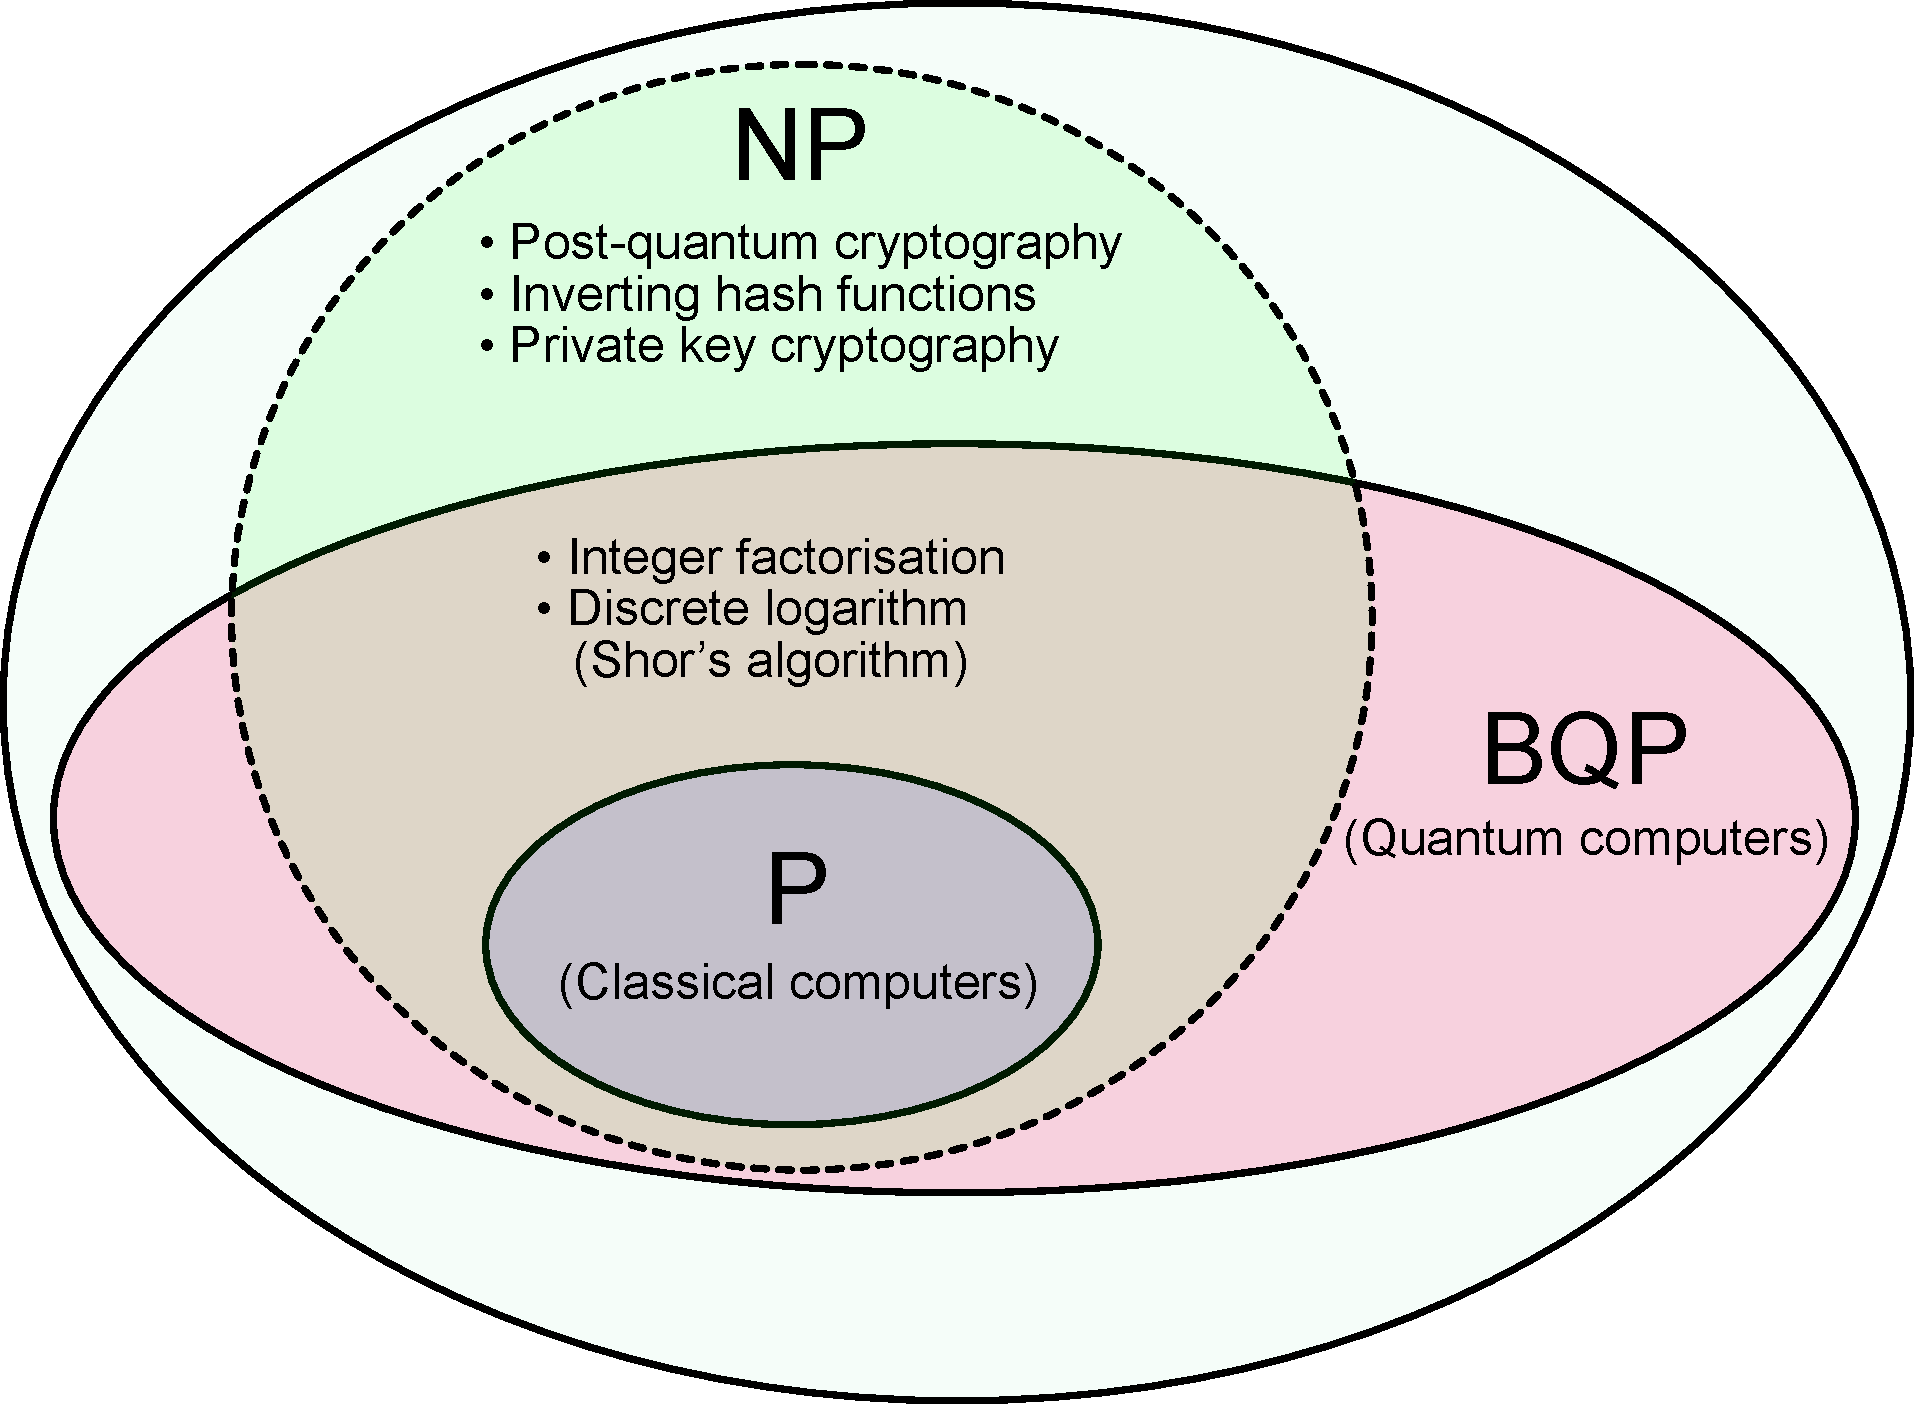
\includegraphics[width=\columnwidth]{figures/Complexity_classes}
	\caption{Venn diagram of the believed relationships between some complexity classes relevant to classical and quantum computing and cryptography. \textbf{P} is the class of problems that can be efficiently solved on a classical computer. \textbf{BQP} is the same for quantum computers. Problems outside \textbf{P} and \textbf{BQP} cannot be efficiently solved by any physically realisable computer (unless the laws of quantum physics are incorrect). Since $\mathbf{P}\subseteq\mathbf{BQP}$, quantum computers can efficiently solve classical problems, but the converse is not believed to be true since it is believed but not proven that $\mathbf{P}\subset\mathbf{BQP}$. \textbf{NP} is the class of problems that can be efficiently verified (as opposed to solved) on a classical computer. While \textbf{P} and \textbf{BQP} are physically realisable computational models, \textbf{NP} is not believed to be, instead being a theoretical one. In general, breaking crypto-systems resides in \textbf{NP} since this can be efficiently verified but not efficiently solved.} \label{fig:complexity}
\end{figure}

If a cryptographic problem is known to reside in \textbf{BQP} but not in \textbf{P}, it can be compromised by quantum computers but not by classical computers. This is where we believe the integer factorisation and discrete logarithm problems reside, which form the basis of current public-key cryptography. Note that neither of these problems has been \emph{proven} to lie outside of \textbf{P} --- it is a strongly held belief based on the fact that these problems have been incredibly well studied. But who knows, perhaps we just haven't studied them hard enough?

For \emph{post-quantum cryptography} (Sec.~\ref{post-quantum-cryptography-pqc}) the ultimate goal is to develop protocols whereby decryption in the absence of knowing the key provably lies outside of \textbf{BQP}. However the field of computational complexity is an extremely challenging one, and many very basic identities are assumed to hold, but not proven to. The most famous example of this is the \textbf{P} versus \textbf{NP} problem, a thorn in the side of computer scientists for decades. Roughly speaking, this statement asks ``if a problem is easy to verify is it easy to solve?'', the answer to which is understood but not proven to be ``no''. The difficulty in proving these complexity relationships often means we have to accept weaker computational security assumptions.
\section{Classical cryptography} \label{classical-cryptography}

There are several cryptographic primitives that are essential building blocks for the information security protocols we all rely upon \cite{bib:Schneier96}.

\subsection{Private-key
cryptography} \label{private-key-cryptography}

Private key cryptography refers to encryption where the same key is used for both encryption and decryption, a property that has led to such schemes also being referred to as \emph{symmetric} ciphers.

For a given message $m$, key $k$ and ciphertext $c$, the encryption and decryption operators satisfy the properties,
\begin{align}
	{\tt enc}_k(m) &\to c, \nonumber\\
	{\tt dec}_k(c) &\to m, \nonumber\\
	{\tt dec}_k \circ {\tt enc}_k(m) &= m, 
\end{align}
where $\circ$ denotes operator composition.

Modern private-key cryptographic standards, such as AES-256, are considered but not proven to be safe against future quantum computers as they are not believed to exhibit any inherent mathematical structures that quantum computers can efficiently exploit. They additionally have the advantage of being algorithmically very fast, and do not incur any overhead in encrypted message size --- plaintexts and ciphertexts are typically of the same size. This is in contrast to public key cryptography, where ciphertexts are significantly larger than plaintexts.

Despite these advantages symmetric ciphers are not very practical to utilise in isolation as they require secrecy when exchanging secret keys for future use. When communicating with someone a long distance away who we aren't able to meet in a dark back alley, this becomes impractical, requiring public-key cryptography for the purposes of key exchange.

Block and stream ciphers are optimal for different use cases. For example, when dealing with files or latency-independent data versus real-time, low-latency data streams.

Private-key encryption comes in two general flavours: \emph{block ciphers} and \emph{stream ciphers}. 

\subsubsection{Block ciphers}

Block ciphers act on fixed-size blocks of data, mapping them to ciphertext blocks, typically of equal size. For example, AES-256 takes blocks of data and keys of length 256 bits, generating ciphertext blocks of the same length. In the case of equal plaintext and ciphertext block sizes this implies the encryption/decryption operations implement a bijective map or permutation between the space of plaintexts and ciphertexts. This structure is shown in Fig.~\ref{fig:block_cipher}.

Block ciphers such as the AES suite of ciphers tend to be more widely used than stream ciphers.

\begin{figure}[!htb]
	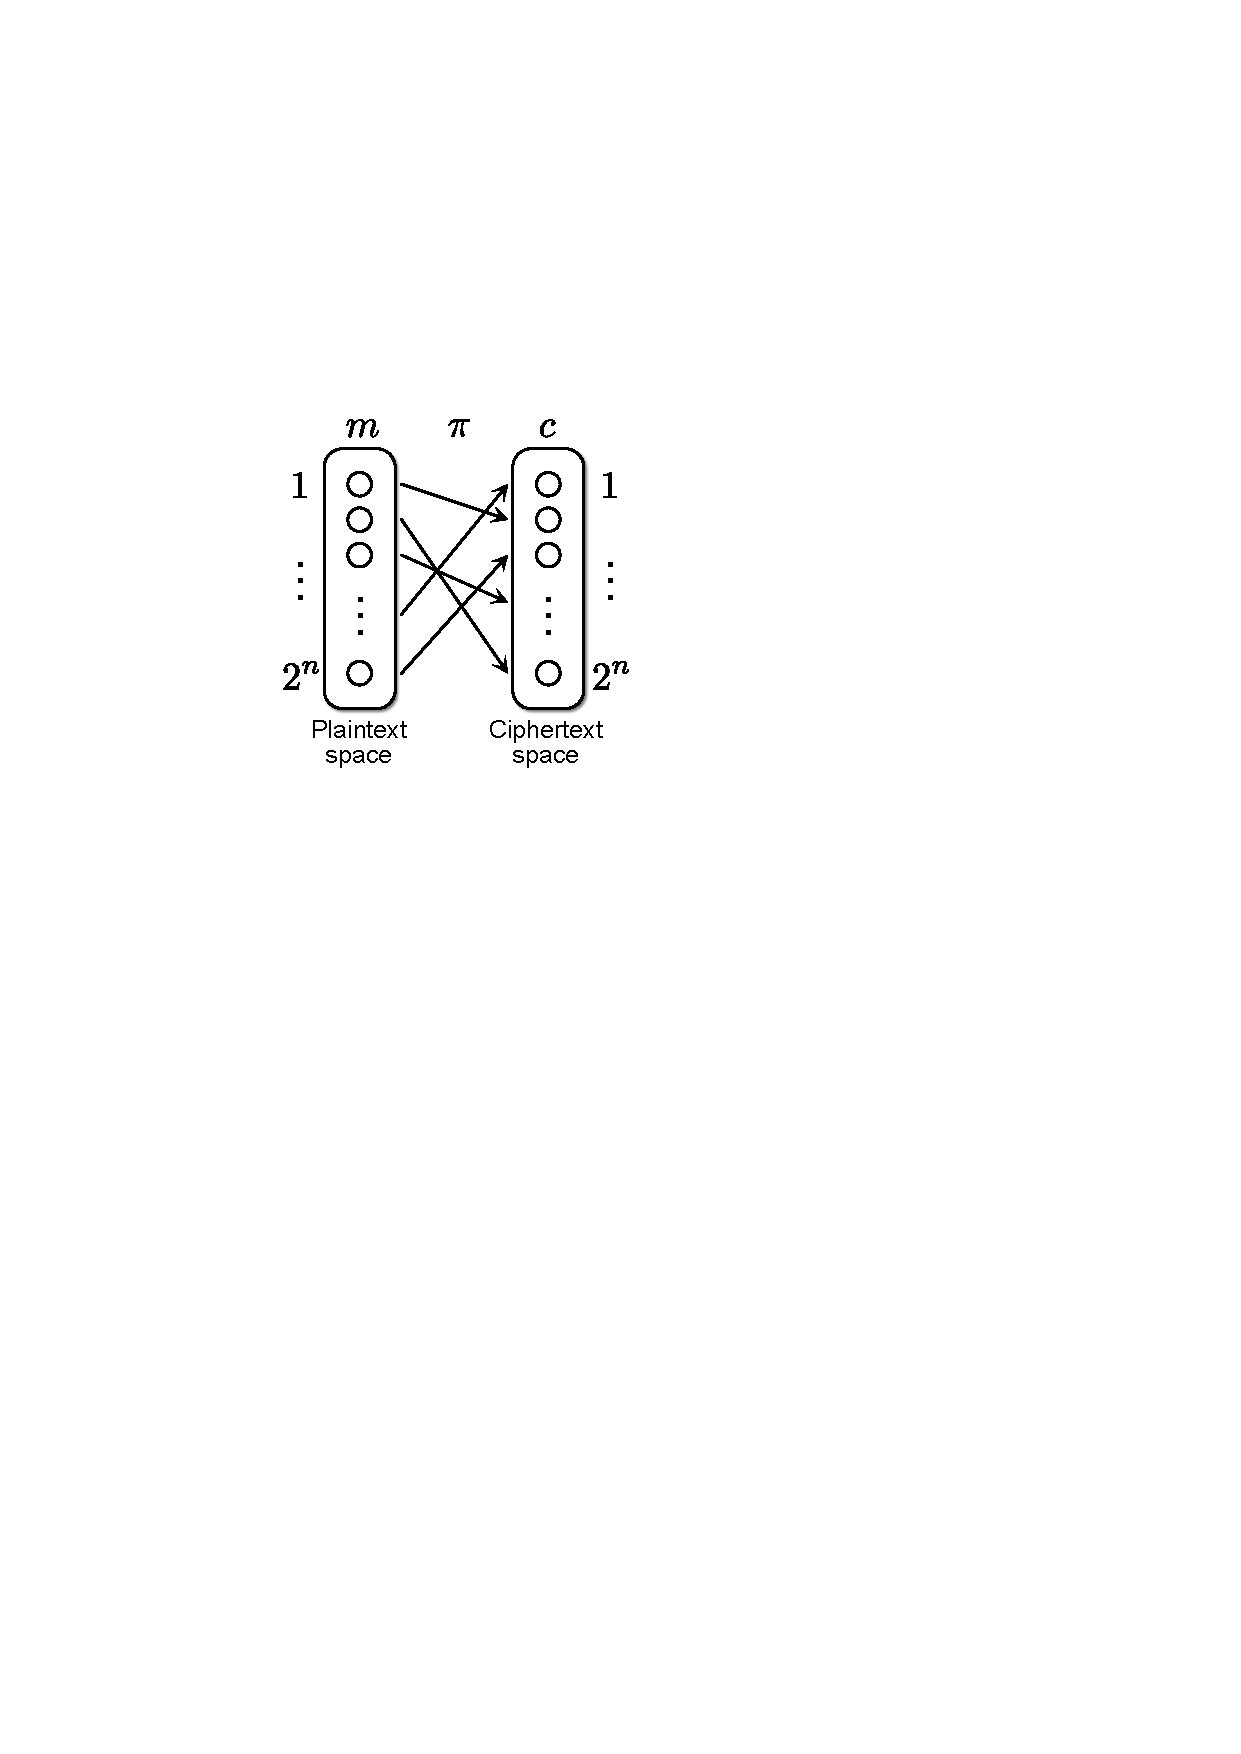
\includegraphics[width=0.5\columnwidth]{figures/block_cipher}
	\caption{Structure of a block cipher. For a block size of $n$ bits there are $2^n$ possible plaintexts, similarly for ciphertexts. Since every plaintext ($m$) must uniquely map to a distinct ciphertext ($c$), it follows via a pigeonholing argument that the encryption operation is effectively defined as a bijective map $\pi$ between the two spaces, such that $\vec{c}=\pi\cdot \vec{m}$.} \label{fig:block_cipher}	
\end{figure}

\subsubsection{Stream ciphers}

Stream ciphers act on data streams as opposed to blocks, with no inherent constraints on the size of the data. Here the data-stream is bitwise XORed with a pseudo-random sequence generated from the key and data-stream history, providing significant similarities with the one-time-pad (Sec.~\ref{one-time-pad-encryption}).

Although stream ciphers are useful for low-latency applications, they are less robust against errors than block ciphers. In a block cipher, an error within a plaintext (ciphertext) block will remain contained in the corresponding ciphertext (plaintext) block. In a stream cipher, on the other hand, any introduced errors will propagate indefinitely through the remainder of the stream owing to the intrinsic feedback loop, making error recovery challenging.

The structure of a stream cipher is shown in Fig.~\ref{fig:block_cipher}.

\begin{figure}[!htb]
	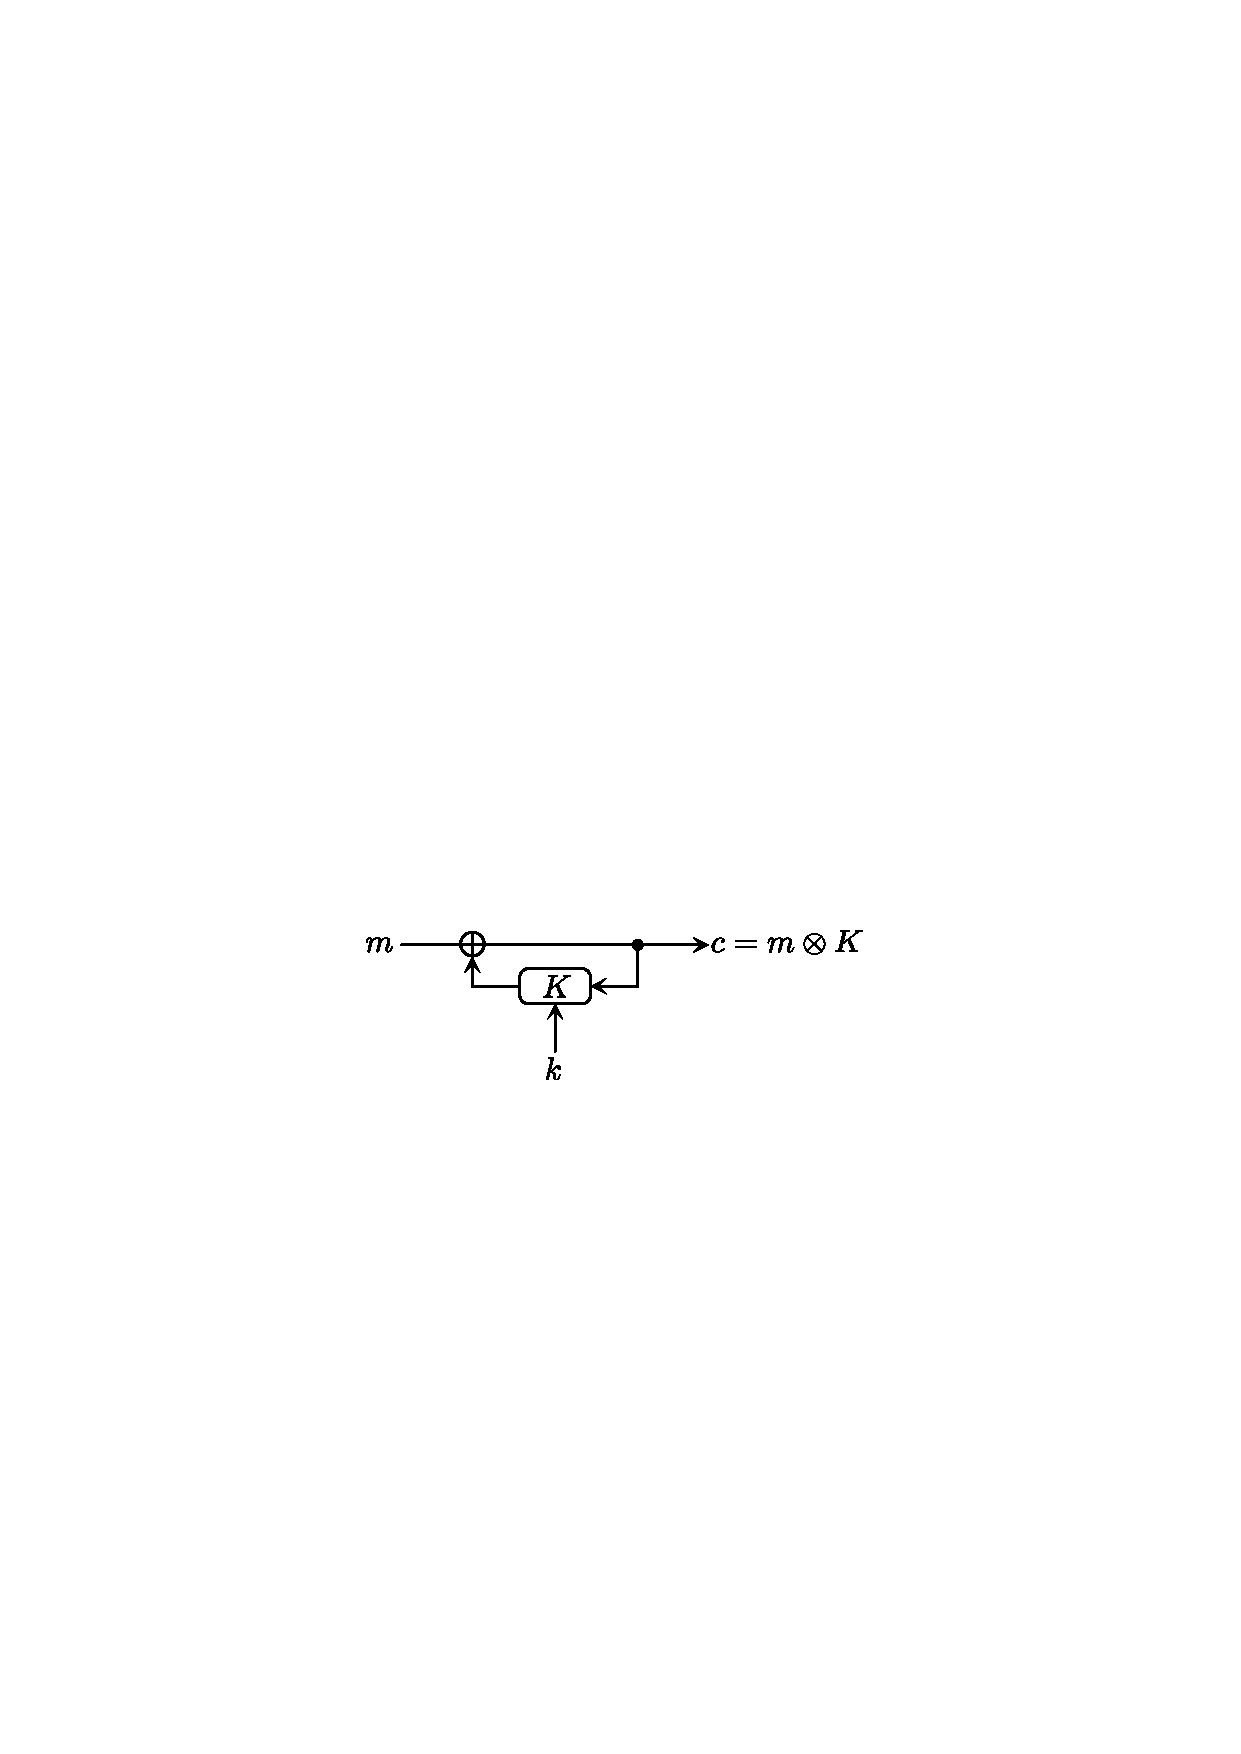
\includegraphics[width=0.8\columnwidth]{figures/stream_cipher}
	\caption{Structure of a stream cipher. A message stream $m$ is mapped to a ciphertext stream $c$ via XORing with a pseudorandom string $K$, $c=m\otimes K$. $K$ is derived as a function of the key $k$ and feedback from the previously encrypted output stream.} \label{fig:stream_cipher}	
\end{figure}

\subsubsection{One-time-pad encryption} \label{one-time-pad-encryption}

Of all the classical ciphers there is one and one only that exhibits perfect information-theoretic security, the one-time-pad (OTP) or Vernam cipher. The OTP, however, is an especially impractical symmetric cipher that requires a key as long as the message which can only be used once (hence the name).

Mathematically, the encryption and decryption operations are trivial to implement, simply bitwise XOR operations applied between the message and key to yield the ciphertext,
\begin{align}
	c = m \oplus k,
\end{align}
or between ciphertext and key to recover the message,
\begin{align}
	m = c \oplus k.
\end{align}
Note that the encryption and decryption operations are symmetric since,
\begin{align}
	{\tt enc}_k(m) = {\tt dec}_k(m) = m \oplus k.
\end{align}

But why is this extremely simple cipher perfectly secure? Consider trying to perform a brute-force attack against a ciphertext $c$ by exhaustively trying out every possible key $k_i$. Each $k_i$ will decrypt $c$ to a unique message, 
\begin{align}
    m_i = c \oplus k_i,
\end{align}
meaning that every message of the given length is an equally likely outcome, with no statistical biases or structures of any kind to exploit. If your message is $n$-bits in length, there are $2^n$ possible choices of key, which uniquely reproduce all $2^n$ possible $n$-bit messages.

So the most we can learn is the message's length, which admittedly isn't nothing. If a military general is giving orders, the difference in length between the messages `yes' and `no' is significant, although this is something easily obscured by padding messages to form fixed-length packets.

The non-reusability of the key stems from the fact that for two ciphertexts encoded with the same key we have,
\begin{align}
	c_1\oplus c_2 = (m_1\oplus k)\oplus(m_2\oplus k) = m_1 \oplus m_2,
\end{align}
which is the XOR of the two unencrypted plaintext messages, lending itself to a trivial frequency analysis attack.

Despite the impracticality of the one-time-pad cipher, it has found its place in history. During the Cold War, it was known that diplomats would carry suitcases full of OTP keys between embassies, which after being used were destroyed. However, this isn't an approach likely to find widespread utility for pragmatic reasons, unless we find a more practical way of sharing random bit-strings, to be discussed in Sec.~\ref{quantum-key-distribution-qkd}.

\subsection{Public-key cryptography} \label{public-key-cryptography}

The other form of cryptography is public-key cryptography, also known as \emph{asymmetric} cryptography since unlike symmetric cryptography different keys are used for encryption and decryption, known as the public ($k_{\tt pub}$) and private ($k_{\tt priv}$) keys (collectively a key-pair). The public key can only be used for encryption, and the private key only for decryption, yielding the following properties, 
\begin{align}
{\tt enc}_{k_{\tt pub}}(m) &\to c, \nonumber\\
{\tt dec}_{k_{\tt priv}}(c) &\to m, \nonumber\\
{\tt dec}_{k_{\tt priv}} \circ {\tt enc}_{k_{\tt pub}}(m) &= m.
\end{align}

As the name suggests, the public key can be made public while the private key must be kept private. Importantly, it should not be computationally possible to determine $k_{\tt priv}$ from $k_{\tt pub}$, for the obvious reason that if that were possible everyone could decrypt our messages using the published public key.

This property arises through the use of \emph{trapdoor functions} --- functions that are easy to perform in one direction, but hard to invert in the other. If the private key and public keys are related via such a function it means determining the private key from the public key is extremely difficult, whereas the person possessing the private key can easily manufacture the associated public key.

Public-key cryptography overcomes the impracticality we observed with private-key cryptography. We don't need any \emph{a priori} secrecy to share private keys. Instead, we can do everything over public channels.

Public-key ciphers do, however, have some disadvantages. Firstly, they do not preserve message length during encryption, instead inducing significant overheads in message size. Second, they tend to be algorithmically slower than symmetric ciphers. And thirdly, both of the most popular public-key cryptosystems we use today (RSA and ECC) are vulnerable to quantum attacks via variations on Shor's algorithm (Sec.~\ref{shors-algorithm}).

\subsubsection{RSA (Rivest-Shamir-Adleman)} \label{rsa-rivestshamiradleman}

The RSA public-key cryptosystem \cite{bib:RSA}, named after its inventors, was the first well-known public-key cryptosystem. Here the underlying trapdoor function is integer multiplication, specifically the multiplication of large prime numbers. Multiplication is a straightforward thing to do, even for very large numbers. Taking two prime numbers $p$ and $q$ it is easy to calculate $n=pq$. However, the inverse function of factorisation turns out to be far more complex, and indeed prohibitive via all known classical approaches --- given $n=pq$ it is hard to find $p$ and $q$. This is an example of an \textbf{NP} problem not believed to reside in \textbf{P}.

The best-known classical algorithm for factorising large integers is the general number field sieve, which exhibits time complexity,
\begin{align}
	O(e^{c (\log n)^{1/3}(\log\log n)^{2/3}}),
\end{align}
for an integer consisting of $\lfloor\log_2 n\rfloor+1$ bits. For large numbers, this scaling is highly inefficient. For quantum computers, the story is different, as discussed in Sec.~\ref{shors-algorithm} on Shor's algorithm.

In addition to encryption, by reversing the roles of the private and public keys RSA also lends itself to digital signatures.

The disadvantage of RSA public-key cryptography compared to private-key cryptography is twofold:
\begin{itemize}
	\item RSA keys are significantly larger than contemporary private keys. While private keys are often chosen to be 128 or 256 bits in length, RSA keys are typically chosen to be 2,048 to 4,096 bits in length.
	\item Private key encryption algorithms like AES create ciphertext the same length as the plaintext. RSA on the other hand creates ciphertext messages significantly longer than the plaintext.
	\item The RSA algorithm is far more compute-intensive than, say, AES. To address the above problems, RSA is typically used in hybrid form with AES, where RSA public-key cryptography is used to exchange an AES private key, after which all encryption is conducted via the more efficient AES.
\end{itemize}

It should be noted that it has not been \emph{proven} that integer factorisation is a hard problem. Rather, it has been extensively studied and the best-known algorithms are very computationally hard. This is therefore a not-so-strong example of computational security. It cannot be ruled out that better algorithms will be found or that the problem ends up being proven to not be classically hard at all.

\subsubsection{Elliptic-curve cryptography (ECC)} \label{elliptic-curve-cryptography-ecc}

Elliptic-curve cryptography (ECC) is a more recent approach to public-key cryptography, which like RSA can be used both for encryption or digital signatures. Here the trapdoor function relates to the difficulty of finding the discrete logarithm of a particular group.

Specifically, for some group $G$ where $a,b\in G$ and
\begin{align}
a=b^k,
\end{align}
we can write,
\begin{align}
k=\log_b a,
\end{align}
which reads $k$ is the discrete logarithm of $a$ to the base $b$. While not believed to be classically efficient in general (depending on the group $G$), the discrete logarithm problem can be solved efficiently using a variation of Shor's algorithm on quantum computers (Sec.~\ref{shors-algorithm}).

The primary advantage of ECC over RSA relates to efficiency. For the same level of security, ECC keys can be substantially shorter than RSA keys. The ECC algorithm is also more computationally efficient.

\subsection{Key exchange protocols} \label{key-exchange-protocols}

Given that public-key cryptography induces overheads in message size that symmetric ciphers such as AES-256 don't, we can hybridise these approaches to get the best of both worlds.

Rather than using public-key cryptography to encrypt our messages directly, we can instead use it to exchange private keys, which are subsequently used in a symmetric cipher. Such hybrid approaches are the norm, with the Diffie-Hellman algorithm \cite{bib:DiffieHellman} and its subsequent evolutionary variants being widely used.

A conceptual model for using public-key cryptography for key exchange could be described as follows (see Figs.~\ref{fig:KEM_1} \& \ref{fig:KEM_2}):
\begin{itemize}
	\item Alice and Bob share public keys.
	\item They both prepare independent random secret keys ($s_A$ and $s_B$).
	\item Using one another's public keys they exchange secrets.
	\item Now both parties possess both secrets, which can be combined to make a unified shared secret,
		\begin{align}
			s=s_A\oplus s_B.
		\end{align}
\end{itemize}
This isn't exactly how Diffie-Hellmann works, but is conceptually similar.

\begin{figure}[!htb]
	\centering
	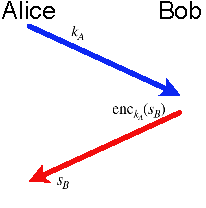
\includegraphics[width=0.75\columnwidth]{figures/Key_exchange_one_way}
	\caption{Two-party key exchange protocol using public-key cryptography. Both parties make their public keys known. Bob uses Alice's public key to securely send her a secret key. (Blue denotes public information, red denotes encrypted information)} \label{fig:KEM_1}
\end{figure}

\begin{figure}[!htb]
	\centering
	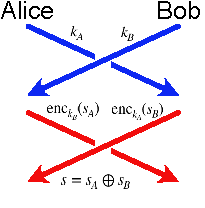
\includegraphics[width=0.75\columnwidth]{figures/Key_exchange_two_ways}
	\caption{Two-party key exchange protocol using public-key cryptography. Both parties make their public keys known, which are used to communicate random secrets with one another. These are combined to yield the master key, which is only compromised if channels in both directions are compromised, making man-in-the-middle attacks more challenging than in Fig.~\ref{fig:KEM_1}. (Blue denotes public information, red denotes encrypted information)} \label{fig:KEM_2}
\end{figure}

These are referred to as \emph{key encapsulation mechanisms} (KEMs) since the private key used for the subsequent symmetric cipher is encapsulated in the message of the asymmetric cipher. Note that in the second model, the shared secret is only compromised if the communication of \emph{both} secrets is compromised, making a man-in-the-middle attack more challenging.

\subsection{Hash functions} \label{hash-functions}

An extremely important class of cryptographic primitives is \emph{hash functions}. A hash function takes an input string $m$ of arbitrary length, and outputs a fixed-length \emph{hash} $h$ (also known as a \emph{checksum} or \emph{digest}),
\begin{align}
	{\tt hash}(m)\to h.
\end{align}

There are several properties we would like functions to exhibit to specifically call them \emph{hash functions}:
\begin{itemize}
	\item Pseudo-randomness: the output to a hash function should appear statistically random and unstructured. Changing a single bit on the input should on average flip half the bits on the output. If you were to use a clock signal as the input, you would have a very good random number generator (this is often exactly how it's done).
	\item Fast to compute: this is a practical issue since we will often want to create checksums for very large pieces of data.
	\item Uniform output probability distribution: averaged over all inputs, all outputs should be equally likely.
\end{itemize}

The use of hash functions is widespread not only within the field of cryptography. For example, checksums can be used for error detection --- when we transmit data we simultaneously transmit its checksum for verification by the recipient.

For cryptographic applications, we desire our hash functions to exhibit some additional properties from which they inherit their cryptographic utility. This leads to the notion of \emph{cryptographic hash functions}, which observe the following additional properties:
\begin{itemize}
	\item \textbf{Pre-image resistance}: for a given hash $h$ it should be computationally difficult to find an input message $m$ that hashes to that value such that ${\tt hash}(m)\to h$.
	\item \textbf{Second pre-image resistance} (aka weak collision resistance): if some message $m_1$ hashes to some value, it should be computationally difficult to find another message $m_2$ that hashes to the same value, such that ${\tt hash}(m_1)={\tt hash}(m_2)$.
	\item \textbf{Collision resistance} (aka strong collision resistance): generalising from the notion of second pre-image resistance, it should be difficult to find \emph{any} two messages that hash to the same value such that ${\tt hash}(m_1)={\tt hash}(m_2)$. When such a pair of messages are found (which must necessarily exist), they are referred to as a \emph{hash collision}.
\end{itemize}

The best-known class of cryptographic hash functions used today is the SHA-2 family of hash functions. This contains several hash functions producing hashes of different lengths, after which they are named. For example, SHA-256 generates a 256-bit hash function.

\emph{Inverse hashing} is the problem of breaking the pre-image resistance of hash functions, finding an input string that hashes to a specified output string,
\begin{align}
	{\tt hash}^{-1}(h)\to m.
\end{align}
For a cryptographically strong hash function, brute-force ought to be the best one can do, which has exponential time complexity.

\subsection{Authentication}

An essential cryptographic primitive is authentication, whereby someone wishes to prove their identity to another party or sign a document to prove that they wrote it, so-called \emph{digital signatures}.

\subsubsection{Authentication using shared secrets} \label{authentication-using-shared-secrets}

If two parties have a pre-existing shared secret (i.e a secret private key) and are confident they are the only ones in possession of it, it becomes trivial to implement a two-party authentication scheme (or signature) using cryptographic hash functions, specifically by exploiting the pre-image resistance property. This can be used to both confirm someone's identity or to sign messages.

\paragraph{Message authentication}

To transmit an authenticated message $m$, Alice transmits to Bob,
\begin{align}
	{\tt auth}(m) = m|{\tt hash}(s|m).
\end{align}
That is, she transmits a message along with a hash of the message and private key. Upon receiving $m$, Bob calculates ${\tt hash}(s|m)$ and checks for consistency between what he calculated and what he received.

This approach not only authenticates the message, but simultaneously serves to detect transmission errors in $m$ by acting as a message checksum, as any errors would change the associated hash.

This technique closely resembles the HMAC (hash-based message authentication code) protocol. The advantage of this approach to authentication lies primarily in efficiency. Public-key signatures (Sec.~\ref{ref:public_key_dig_sig}) are relatively computationally intensive, whereas hash functions are by design highly computationally efficient to evaluate. Combining the two, public-key cryptography could be used for the exchange of a secret key, subsequently utilised by the more efficient HMAC.

\paragraph{User authentication}

Suppose two users in possession of a shared secret key wish to authenticate a channel so as to be convinced they are speaking to one another. This can be achieved using message authentication as a primitive. If Alice wishes to confirm that she is speaking to Bob, she first prepares and signs a random message $m$, sending,
\begin{align}
	{\tt auth}(m) = m|{\tt hash}(s|m).
\end{align}
Bob first calculates ${\tt hash}(s|m)$ to confirm the integrity of the received $m$. If successful, he responds by replying with,
\begin{align}
	{\tt auth}(m|m) = m|m|{\tt hash}(s|m|m),
\end{align}
which Alice is able to evaluate for consistency. Here we have opted for Bob to transmit ${\tt hash}(s|m|m)$ since this creates a hash proving that Bob is in possession of Both $m$ and $s$, but which is distinct from the already transmitted ${\tt hash}(s|m)$. Note that ${\tt hash}(s|m)$ and ${\tt hash}(s|m|m)$ cannot be inferred from one another without knowing $s$.

% For a given message $m$ and shared secret $s$, a signature for $s$ can be made by hashing the concatenated message and secret key,
% \begin{align}
% 	{\tt sig}={\tt hash}(s|m),
% \end{align}
% where the vertical bar represents string concatenation. The other party, also in possession of the shared secret $s$ can easily reevaluate ${\tt sig}$ upon receiving the message $m$. It can easily be seen that a fraudulent signature cannot be made by anyone not in possession of $s$, but additionally the signature can only be verified by someone in possession of $s$, effectively limiting this to two-party scenarios.

% For two parties to confirm that they are speaking to one another the protocol for authentication could proceed as follows:
% \begin{itemize}
% 	\item Alice and Bob both prepare random messages, $m_A$ and $m_B$.
% 	\item They communicate these messages via the channel they want to authenticate.
% 	\item They both calculate \mbox{${\tt sig}_A={\tt hash}(s|m_A)$} and \mbox{${\tt sig}_B={\tt hash}(s|m_B)$} which are shared via the channel.
% 	\item If the values for ${\tt sig}_A$ and ${\tt sig}_B$ calculated by Alice and Bob are consistent with the ones sent by the other it implies the two parties must have possessed the shared secret $s$ and are hence who they say they are.
% 	\item Anyone else possessing $s$ could spoof being the other party and perform a man-in-the-middle attack.
% \end{itemize}

%While this scheme is very robust if the underlying hash function satisfies the pre-image resistance requirement, it relies on a pre-existing shared secret key, which must be shared via other means.

%highly impractical given the requirement that both parties must find the means to share a secret key a priori.

In a multi-user environment with $n$ users, all of whom wish to be able to sign messages with one another, this approach requires on the order of $O(n^2)$ secret keys.

\subsubsection{Public-key digital signatures} \label{ref:public_key_dig_sig}

Despite being very secure, inheriting their security from the pre-image resistance of hash functions, authentication using shared secrets requires first sharing a secret key. Ideally we would like a system with properties akin to public-key cryptography, whereby someone can make available a public key that others can use to verify a signature made with the associated private key. Specifically, we want the following mathematical properties,
\begin{align}
{\tt sign}_{k_{\tt priv}}(m) &\to s, \nonumber\\
{\tt verify}_{k_{\tt pub}}(s) &\to m, \nonumber\\
{\tt verify}_{k_{\tt pub}} \circ {\tt sign}_{k_{\tt priv}}(m) &= m,
\end{align}
where $m$ is the message, $s$ is the signature, and $k_{\tt priv}$ cannot be efficiently determined from $k_{\tt pub}$.

Interestingly, both the RSA and ECC encryption schemes can be used for exactly this purpose, simply by interchanging the roles of the public and private keys. A message is signed by applying RSA/ECC using what is now the private key, which can be decrypted and hence verified (but not forged) using what is now the public key. Now someone producing the keypair has the ability to publish a key that can be used for verification but not signing, whilst keeping the one used for signing secret, which cannot be efficiently determined from one another.

This ability to interchange the roles of keys to use RSA/ECC for digital signatures is more fortuitous than by design, and not something that need hold in general for asymmetric ciphers. Rather, it is specific to RSA/ECC.

As discussed in Sec.~\ref{authentication-using-shared-secrets}, when using shared secrets for authentication, $O(n^2)$ secret keys need to be exchanged (one for each user-pair), highly impractical for many applications. Contrast this with reusable public-key digital signatures in which there need only be $n$ public-keys (one for each user), which can be communicated via public channels with no need for any secret exchanges. This makes public-key digital signatures far more versatile and practical than authentication using shared secrets.

However, in the same way that RSA/ECC encryption may be compromised using Shor's algorithm, so too can RSA/ECC digital signatures. In this instance, a successful Shor attack would allow messages to be fraudulently signed as opposed to decrypted.

In the quantum era, where Shor attacks are viable, it will therefore be necessary to transition to post-quantum digital signatures, to be discussed in Sec.~\ref{post-quantum-cryptography-pqc}. In the same way that quantum cryptography only enables private-key cryptography, there are no known quantum digital signature schemes satisfying our desired properties.

\subsection{One-time passwords (OTP)}

When manually logging into websites using a password, many sites now provide the option or require the use of two-factor authentication (2FA), where in addition to the password some other secondary mechanism is used to confirm identity. These are commonly implemented using one-time passwords (OTPs). In some instances these are communicated by SMS text messages or email. In others it is implemented using time-based one-time passwords (TOTPs), which we describe here.

When configuring an account, in addition to the primary password, a shared secret is established between the client and server, using conventional KEMs, as described previously. The shared secret is held on the client's device but not directly visible to the user. The TOTP is calculated by hashing the shared secret with a timestamp, such that the TOTP is constantly evolving as a function of time, but in a way which does not disclose the shared secret nor the TOTP at other times. Specifically,
\begin{align}
\mathtt{TOTP} = \mathtt{hash}(k|t),	
\end{align}
where $k$ is the shared secret key, and $t$ is a timestamp rounded off to some pre-agreed increment. Here the hash function is typically chosen to produce a short hash of say six decimal digits or so for the purposes of practicality.

Note that via the pre-image resistance of the hash function, establishing the shared secret key $k$ from the TOTP is not viable. Since the TOTP is a hash and only used once, it needn't be encrypted.

Since TOTPs rely on the establishment of a secret key, they could in principle be implemented using quantum key distribution, described in Sec.~\ref{quantum-key-distribution-qkd}.

\subsection{Ratchets} \label{ratchets}

The risk of man-in-the-middle attacks is one that is difficult to rule out. But despite being impossible to discount, we can make life harder for them by giving them more work to do. Suppose the attacker didn't just have to perform an intercept-resend attack once to read a single message, but instead was required to spoof all messages from the message history. This would require a much more consistent and committed effort by the adversary. This introduces the notion of \emph{ratchets}, whereby keys at all points in time must be compromised to break security (see Fig.~\ref{fig:ratchet}).

The idea of ratchets has been popularised by the Signal protocol \cite{bib:SignalProtocol}, used in the Signal messaging app. The goal of this technique is to both improve security and provide so-called \emph{forward secrecy} and \emph{backward secrecy}:
\begin{itemize}	
	\item Forward secrecy: when a user stops participating in a communication (i.e they are denied future session keys) they are unable to decrypt future messages.
	\item Backward secrecy: compromising the current key does not unlock past messages or the present one if past keys are not also known.
\end{itemize}

The approach here is for communicating parties to hold a local \emph{state register} on their device. For every communication, a new key is exchanged. The session key actually used to encrypt the communication is obtained by hashing together the state register and the newly exchanged key. The register is then updated to hold this session key for the next round,
\begin{align}
	s_n=\texttt{hash}(k_n|s_{n-1})
\end{align}

\begin{figure}[!htb]
	\centering
	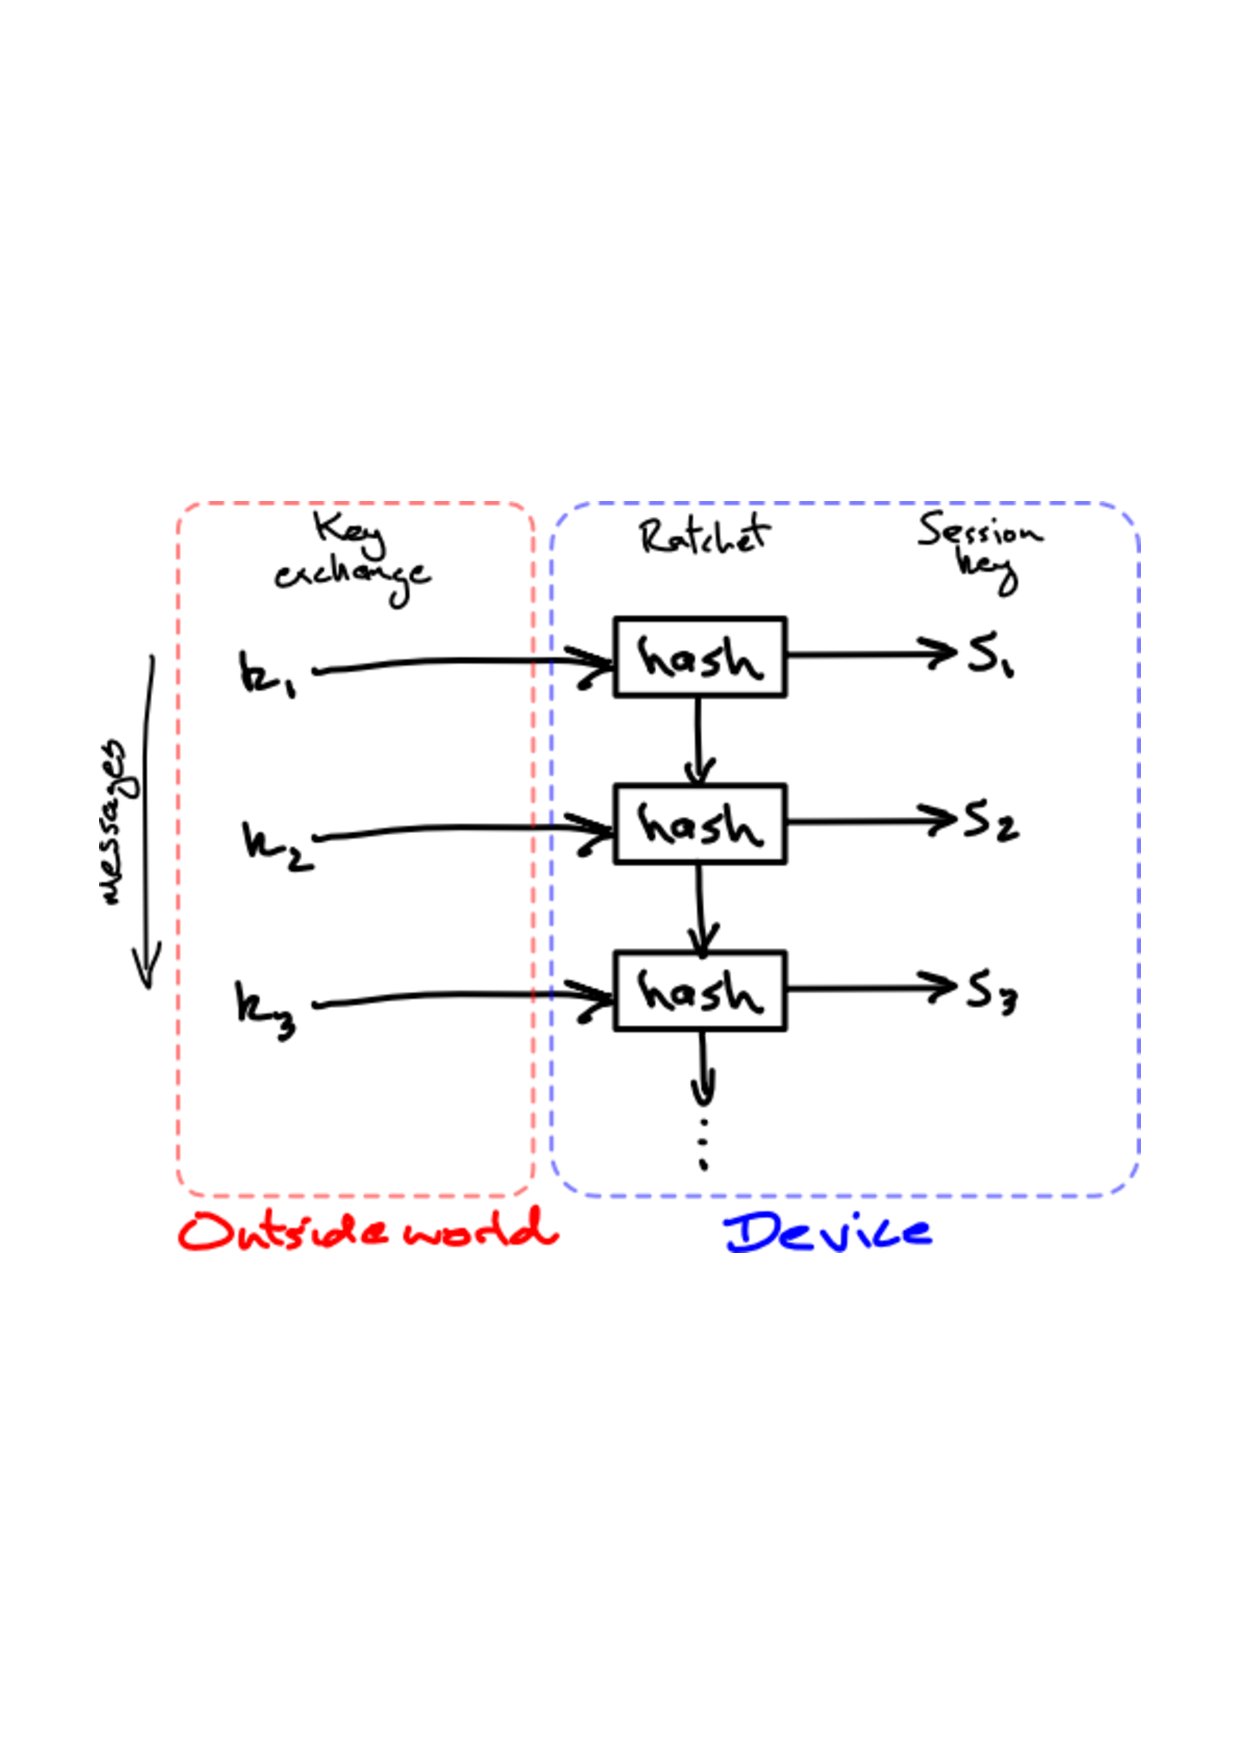
\includegraphics[width=\columnwidth]{figures/Ratchet}
	\caption{A simple ratchet mechanism whereby the current session key is derived from a hash of the most recently exchanged key and the previous session key. This mechanism provides both forward and backward secrecy, and ensures that a session key can only be compromised if all previously exchanged keys were compromised.} \label{fig:ratchet}
\end{figure}

From the diagram above it is evident via the pre-image resistance of the hash function, that intercepting some key $k_n$ does not allow the session key $s_n$ to be determined unless the state register is known, which is a function of all previous session keys. That is, all exchanged private keys must have been intercepted to determine the current session key. This provides our backward secrecy.

Similarly, if this were a group communication and a party stopped receiving newly exchanged keys, they would not be able to determine future session keys, thereby providing our forward secrecy.

The introduction of ratchets significantly complicates life for adversaries attempting to perform man-in-the-middle attacks and one of the reasons the Signal protocol is deemed so secure (see Fig.~\ref{fig:musk}).

\begin{figure}[!htb]
	\centering
	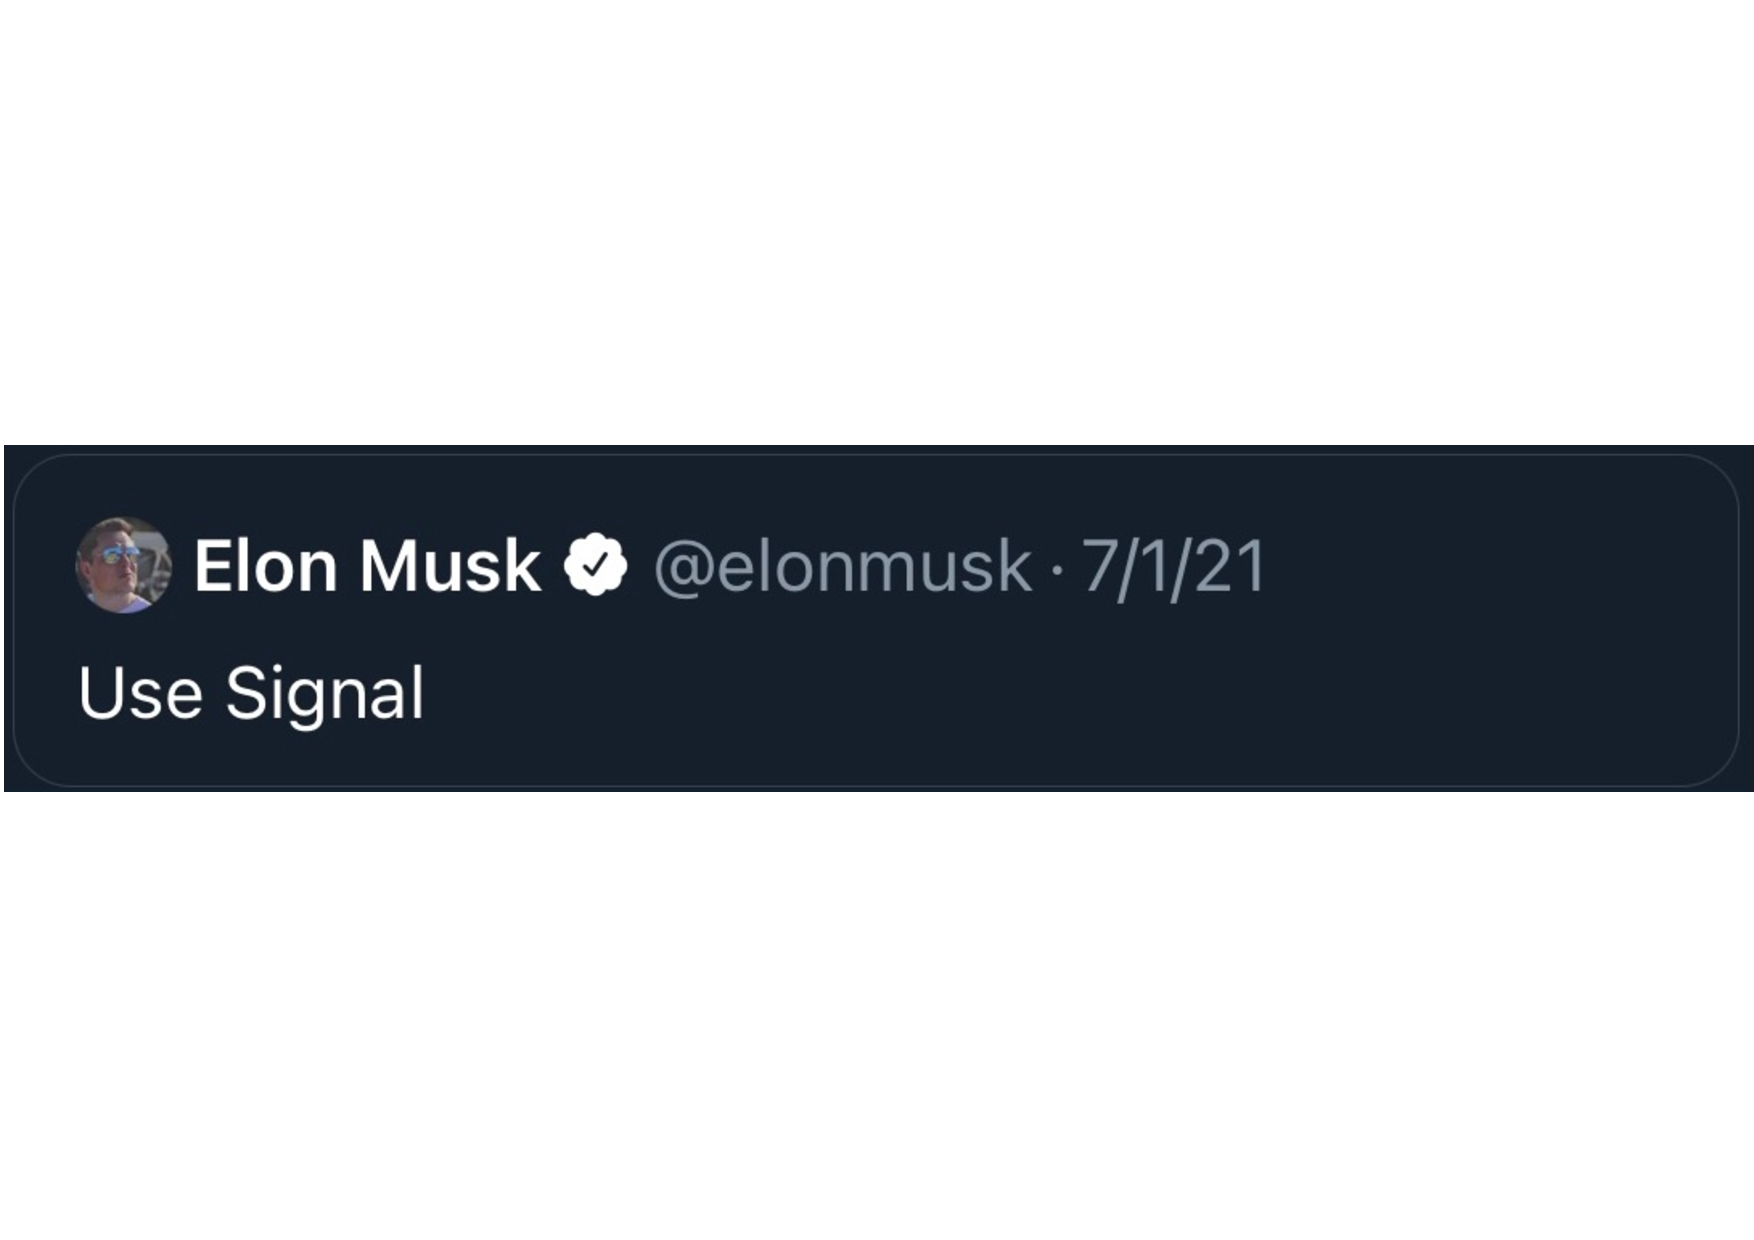
\includegraphics[width=\columnwidth]{figures/Musk}
	\caption{Elon Musk's views on the Signal messaging app.} \label{fig:musk}
\end{figure} 

\subsection{Zero-knowledge proofs (ZKPs)}

A \textit{zero-knowledge proof} (ZKP) is an interactive protocol between two parties --- a \textit{prover} Peggy, and a \textit{verifier} Victor --- where Peggy wishes to efficiently prove to Victor that she knows the solution to a problem, without actually revealing the solution. Thus, a ZKP can serve as a signature that a problem has been faithfully solved, without disclosing the solution.

ZKPs are useful in a number of cryptographic applications, most notably in authentication. In the case of classical computing, a variety of free software packages are available for compiling ZKPs for generic code. However, ZKPs become far more valuable in the case of cloud quantum computing, where there is an inherent complexity asymmetry between the client Victor (classical resources only) and the server Peggy (full quantum resources), whereby efficient ZKPs become a useful transactional tool during computational outsourcing. In a commercial context, a client can convince themselves that a server has actually performed an outsourced computation before finalising the transaction.

\subsubsection{Graph isomorphism}

A conceptually simple example for illustrating the operation of a ZKP protocol is the \textit{graph isomorphism problem}. Two graphs are \textit{isomorphic}, denoted \mbox{$G_1\sim G_2$}, if there exists a permutation \mbox{$\pi\in S_n$}\footnote{In group theory, $S_n$ denotes the symmetric group, the set of all permutations on $n$ elements, of which there are \mbox{$|S_n|=n!$} (the order of the group).} on their vertex labels that makes them equivalent, i.e \mbox{$G_1=\pi\cdot G_2$}\footnote{Here we have employed the operator notation that \mbox{$\pi\cdot G$} means `permutation $\pi$ applied to graph $G$'. Alternately, in matrix notation, where $\pi$ is a permutation matrix and $G$ is an adjacency matrix, this operation implies the matrix conjugation \mbox{$\pi\cdot G\cdot\pi^\top$}.}. The graph isomorphism problem is to find $\pi$ for arbitrary $G_1$ and $G_2$.

This problem is clearly contained in \textbf{NP}, since permuting vertices in graphs and directly comparing them are both computationally straightforward, making verification of the problem a polynomial-time affair. However, it is believed that explicitly determining the respective permutation is difficult in general. This is intuitively unsurprising, since for a graph with $n$ vertices, there are $n!$ possible permutations to consider (which is super-exponential), and therefore a na{\" i}ve brute-force approach would require $O(n!)$ comparisons in the worst-case\footnote{This is the worst-case scenario. In many special cases, knowledge of the underlying graph structure can simplify this enormously, yielding classically efficient runtimes.}. This problem is not believed to be contained in either \textbf{P} or \textbf{NP}-complete, and therefore presumed to be \textbf{NP}-intermediate.

\begin{figure}[!htpb]
	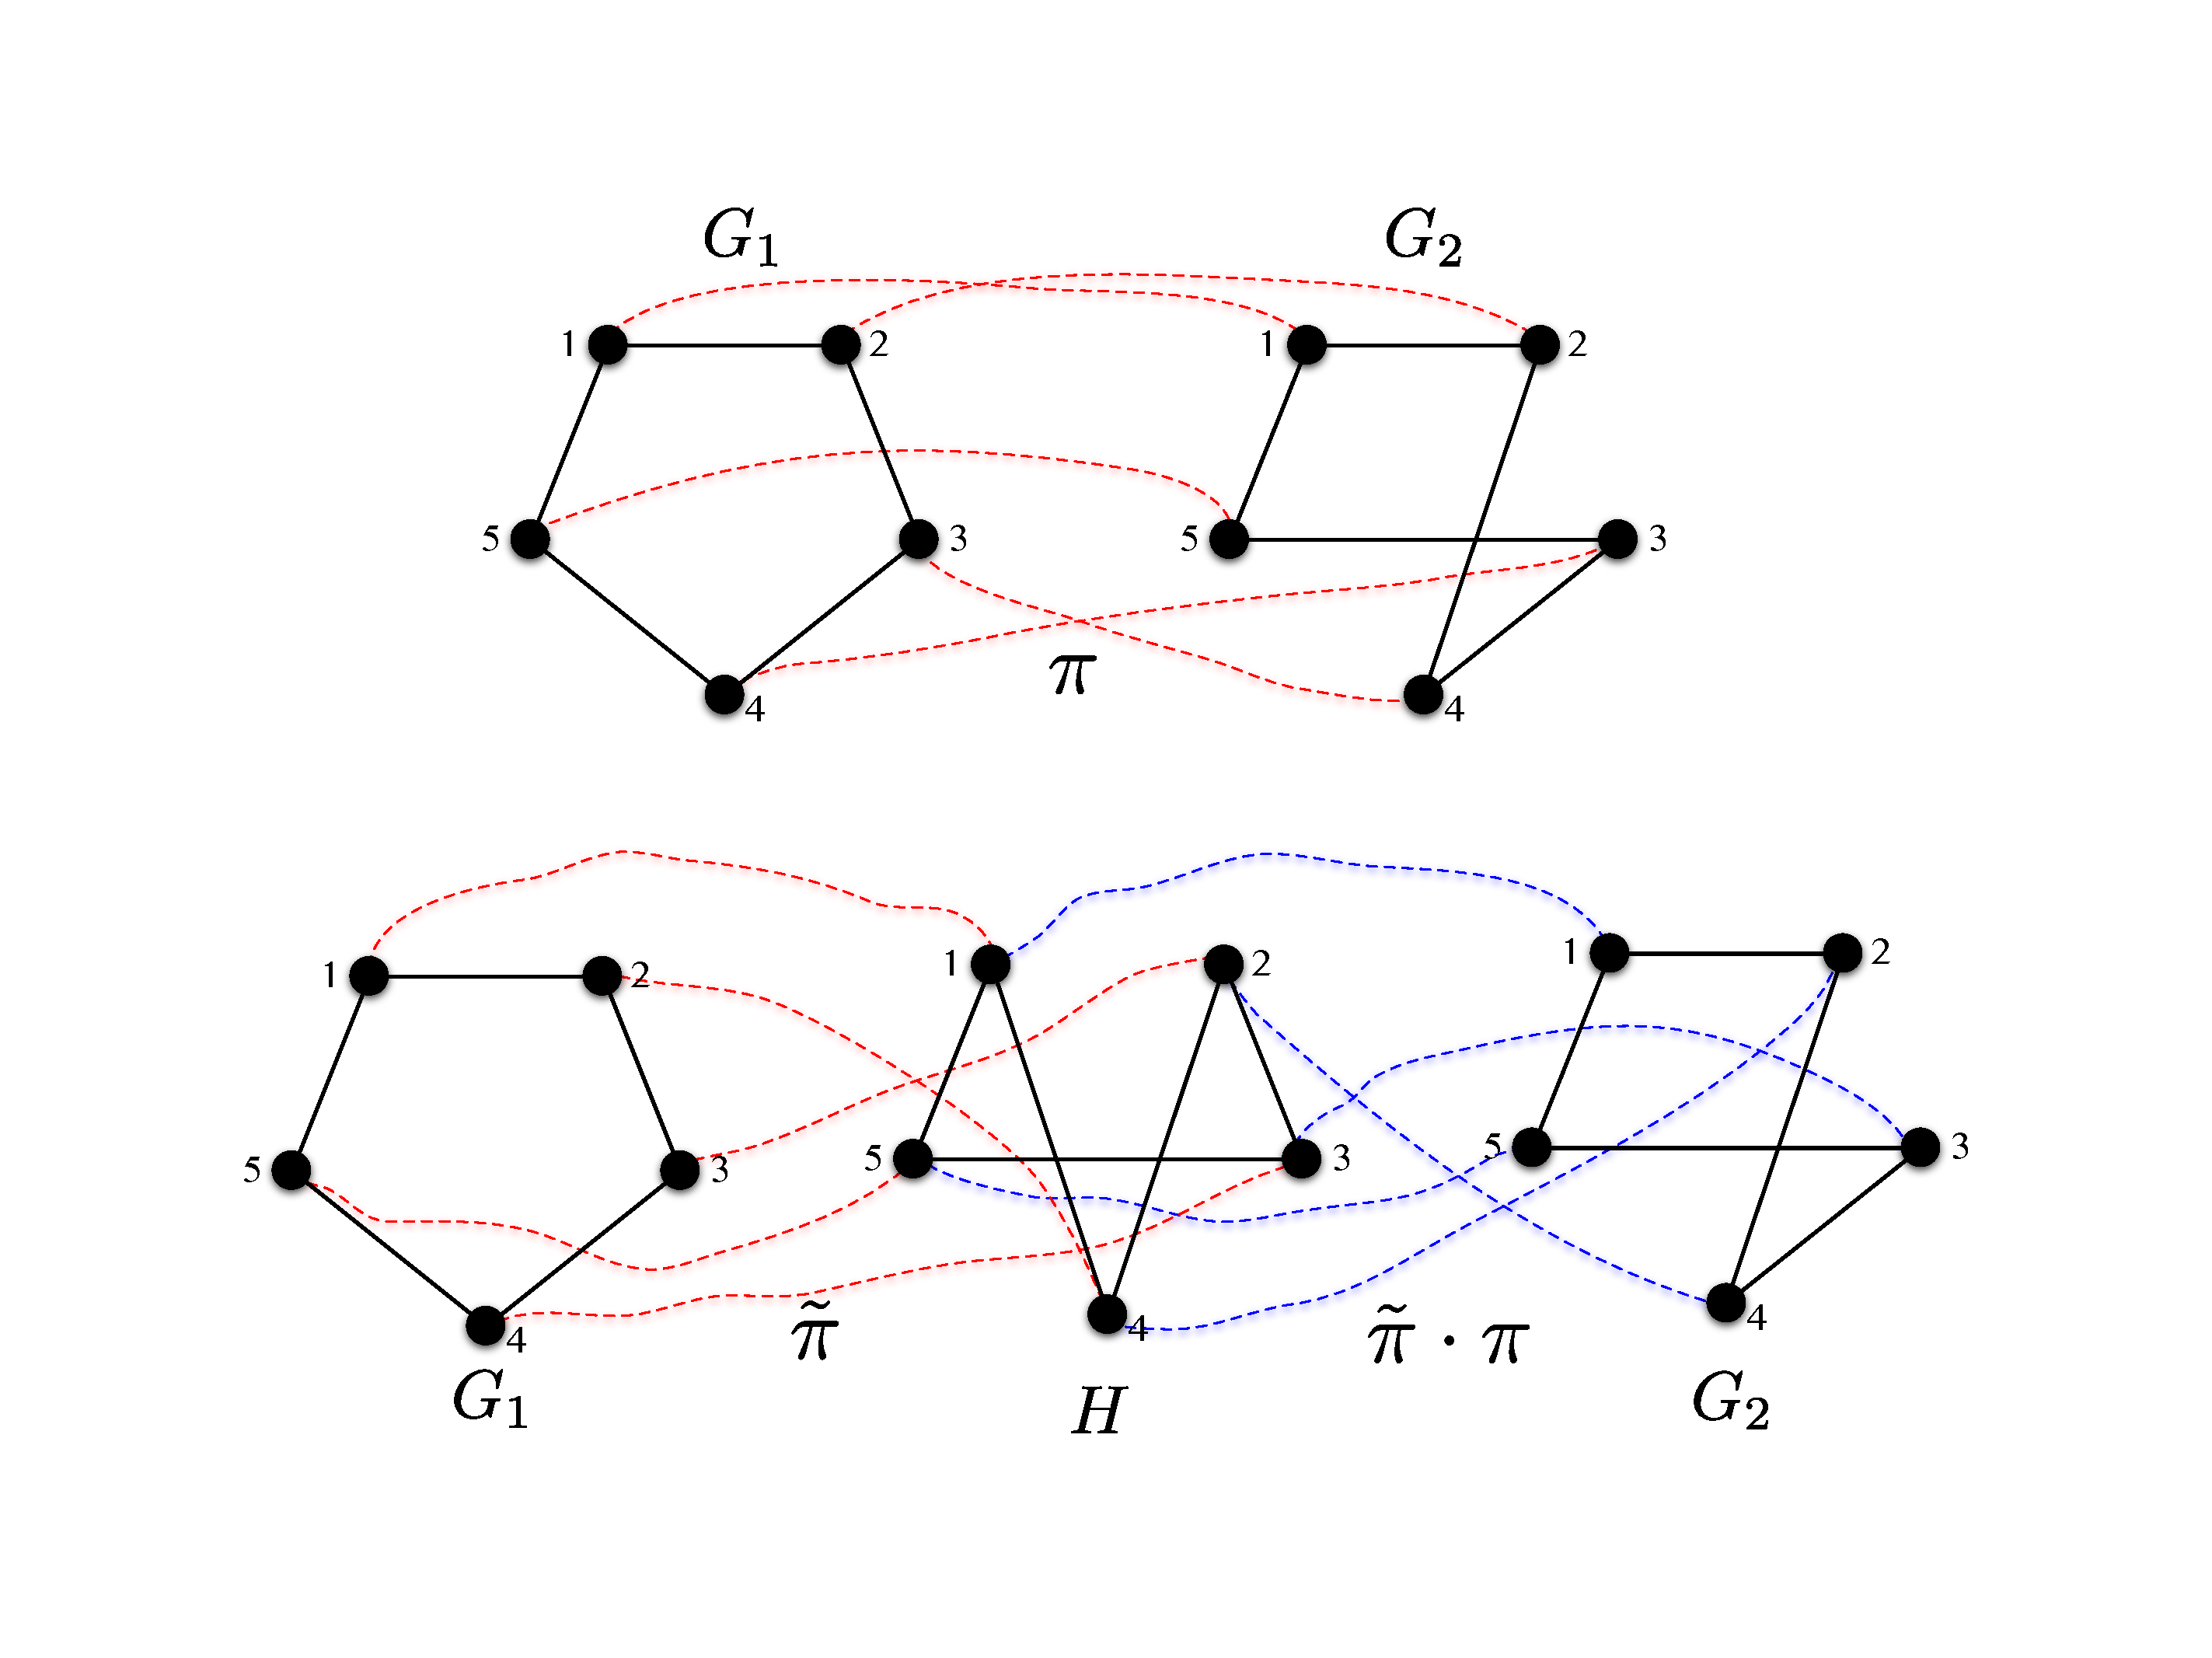
\includegraphics[width=\columnwidth]{figures/ZKP_graph_isomorphism}
    \caption{The isomorphisms \mbox{$G_1\sim G_2$} (top), and \mbox{$G_1\sim H\sim G_2$} (bottom). Coloured lines indicate the vertex relabelings associated with the respective isomorphisms. Knowing the isomorphisms \mbox{$G_1\sim H$} and \mbox{$G_2\sim H$} simultaneously implies knowledge of \mbox{$G_1\sim G_2$} via composition of the permutations. However, knowing only one of them does not, since $H$ is chosen randomly. By repeatedly, randomly proving knowledge of one of the two isomorphisms with $H$ we achieve asymptotic certainty that the prover must have known \mbox{$G_1\sim G_2$}, without actually revealing the associated permutation $\pi$.}\label{fig:ZKP_graph}
\end{figure}

In the example isomorphism presented in Fig.~\ref{fig:ZKP_graph}(top), the vertex permutation mapping $G_1$ to $G_2$ could be expressed in vector form as,
\begin{align}
\pi = \begin{pmatrix}
	1 \\
	2 \\
	3 \\
	4 \\
	5
\end{pmatrix}_{G_1} \to \begin{pmatrix}
	1 \\
	2 \\
	4 \\
	3 \\
	5
\end{pmatrix}_{G_2},
\end{align}
where indices denote vertex labels, or equivalently via the permutation matrix,
\begin{align}
\pi = \begin{pmatrix}
	1 & 0 & 0 & 0 & 0 \\
	0 & 1 & 0 & 0 & 0 \\
	0 & 0 & 0 & 1 & 0 \\
	0 & 0 & 1 & 0 & 0 \\
	0 & 0 & 0 & 0 & 1
\end{pmatrix}.
\end{align}

\begin{figure}[!htb]
\begin{mdframed}
\texttt{
function ZKP.GraphIsomorphism($G_1$, $G_2$):
\begin{enumerate}
	\item Graphs $G_1$ and $G_2$ are known to both verifier Victor and prover Peggy.
	\item Peggy knows the permutation $\pi$ for the isomorphism \mbox{$G_1\sim G_2$},
	\begin{align}
		G_1 = \pi \cdot G_2.
	\end{align}
	\item Peggy wishes to prove to Victor that she knows $\pi$, without disclosing what it is.
	\item Peggy chooses another random permutation $\tilde\pi$, and constructs the new permuted graph $H$,
	\begin{align}
		H &= {\tilde\pi}\cdot G_1\nonumber\\
		& = {\tilde\pi}\cdot \pi \cdot G_2.
	\end{align}
	\item Peggy shares $H$ with Victor, randomly isomorphic to both $G_1$ and $G_2$.
	\item Victor randomly (with probability \mbox{$p=1/2$}) asks Peggy to prove \textit{either} \mbox{$H\sim G_1$} or \mbox{$H\sim G_2$}.
	\item She accordingly reveals either $\tilde\pi$ or \mbox{$\tilde\pi\cdot\pi$} to Victor. He can now efficiently verify either \mbox{$H\sim G_1$} or \mbox{$H\sim G_2$} respectively, by performing the inverse permutation,
	\begin{align}
		G_1 &= {\tilde\pi}^{-1} \cdot H,\nonumber\\
		G_2 &= ({\tilde\pi}\cdot \pi)^{-1} \cdot H.
	\end{align}
	\item Victor is unable to determine $\pi$ from either scenario alone, but could were he to know \textit{both} isomorphisms simultaneously, since,
	\begin{align}
		\pi = {\tilde\pi}^{-1}\cdot (\tilde\pi\cdot\pi).
	\end{align}
	\item The above is repeated $n$ times. Each time, Peggy chooses a new random $\tilde\pi$.
	\item If Peggy does not actually know $\pi$, the probability of fraudulently passing this test $n$ times is,
	\begin{align}
		P_\text{deceive} = \frac{1}{2^n}	.
	\end{align}
	\item With confidence \mbox{$1-P_\text{deceive}$}, Victor knows that Peggy knows $\pi$, without knowing it himself.
	\item $\Box$
\end{enumerate}}
\end{mdframed}
\caption{A zero-knowledge proof for the graph isomorphism problem. Victor (verifier) provides two graphs to Peggy (prover), who can demonstrate with asymptotic certainty that she knows their isomorphism, without disclosing the associated permutation relating them.} \label{alg:ZKP_graph}
\end{figure}

To provide a ZKP for this, Peggy's goal is to prove that she knows $\pi$, without explicitly revealing it. An efficient, randomised, classical ZKP protocol for achieving this is provided in Fig.~\ref{alg:ZKP_graph}, and a specific example illustrated in Fig.~\ref{fig:ZKP_graph}. The key underlying principle here is to obscure $\pi$ through randomisation, whereby instead of directly proving knowledge of $\pi$, it is implied via multiple proofs of isomorphisms with intermediate random graphs.

\subsubsection{Hash functions}

Hash functions can be used to prove knowledge of a piece of data. If Alice and Bob both possess data $x$ then Alice can prove to Bob that she knows $x$ by revealing,
\begin{align}
y=\texttt{hash}(x).
\end{align}
This acts as a signature for $x$ from which $x$ itself cannot be determined owing to the pre-image resistance of the hash function.

This can additionally be used in a different context where Alice wishes to provide a public proof that she knows $x$ now, but doesn't wish to disclose $x$ itself until later. When at a later point in time she does reveal $x$, its previously published hash proves retrospectively that she knew it at the time of publishing $y$. This is sometimes referred to as \emph{commitment} and an important primitive especially in blockchain implementations.

By combining this technique with a digital signature scheme, if Alice signs the hash at the time of publication this additionally serves to prove her identity as the one who published it.

\subsubsection{Digital signatures}

Digital signatures on their own are also a form of ZKP, where identity is being proven. Since the private and public keys forming the key-pair are related by a trapdoor function, providing a digital signature (which can be verified using the public key) provides proof of ownership of the associated private key (which represents the user's identity and should be kept secret).
\section{Classical attack vectors} \label{classical-attack-vectors}

Any cryptosystem is vulnerable to attacks and this piece wouldn't exist if they weren't. Attacks come in many shapes and forms, some computational, others not. We begin by discussing classical attack vectors, which refers to attacks using only classical resources, which may or may not be computational in nature.

\subsection{Backdoors} \label{backdoors}

By far the most powerful classical attack vectors are \emph{backdoors}, whereby cryptography is bypassed altogether, providing direct access to plaintext data. This could be achieved in a number of ways:
\begin{itemize}
	\item Malware could be installed onto clients' devices that directly accesses plaintext data streams and sends them to the attacker. Malware could find its way onto devices via malicious code (e.g that link you pressed on that strange SMS you received), or directly installed, as has often been the case by human intelligence (HUMINT) agencies penetrating physical security measures. Malware attacks can indeed offer far greater utility than simply intercepting data, and can be used to control client devices for other purposes, including sending fraudulent data. Perhaps the most famous example of malware being used by a nation-state was Israel's installation of the Stuxnet malware onto the computers controlling Iran's nuclear centrifuges, destroying a significant number of them, setting back Iran's nuclear program by years according to some estimates.
	\item Targets are tricked into using encryption algorithms that have vulnerabilities known to the attacker but no one else. It has often been speculated that the NSA manipulated standardised encryption algorithms to this end, although this has not been firmly established.
	\item Governments use their legislative power to force computer hardware and software manufacturers to hard code backdoors into devices granting government agencies direct access to client-side data. This is effectively a malware attack by decree, but one only available to governments with jurisdictional power over the companies manufacturing devices. World governments have for a long time become increasingly hostile to the availability of strong end-to-end encryption on consumer-grade devices, with a long history of lobbying the tech sector to introduce backdoors, lamenting the missed opportunities for law enforcement and intelligence agencies. Although not admitted, it should be taken for granted that such backdoors exist in major commercial operating systems and hardware. For example, as described in \href{https://peterrohde.org/apples-child-protection-software-is-not-about-child-safety-its-a-government-backdoor/}{this article}, Apple's child safety framework by the nature of its design is a clear client-side, government backdoor, and by virtue of the people implementing it clearly isn't something that's intended with child safety as the leading priority (although using the justification `child safety' is the leading way to shut down any political opposition to it and inhibit transparency into what data is collected).
\end{itemize}

Backdoors in any incarnation can be regarded as \emph{post-quantum attack vectors} --- if you have direct access to client-side data it simply doesn't matter how strong your encryption with other parties is. Bearing in mind that any system is only as secure as any single point of failure --- of which backdoors are one --- this is a type of attack that transcends eras and technologies, and must always be a priority in secure systems.

One of the strongest protections against backdoors is to rely on open-source software (both for operating systems and applications), allowing anyone to independently audit the code with complete transparency. This is one of the leading reasons why the security of open-source messaging apps such as Signal is considered more robust and reliable than proprietary, closed-source apps which lack this transparency and the ability for independent auditing.

\subsection{Side-channel attacks} \label{side-channel-attacks}

A side-channel attack is one that exploits differences between the theory and implementation of a cryptosystem. Theory almost always makes highly idealised assumptions which are difficult to perfectly reflect in practise. Should these differences provide correlations that can be exploited to gain secret information, it provides avenues for attack. Side-channel attacks exist both for classical and quantum cryptography, however quantum systems are arguably more vulnerable due to the greater difficulties in making experiment perfectly match theory and that classical systems are far better studied.

\subsection{Hammer attacks} \label{hammer-attacks}

One of the most successful classical attack vectors, effectively a form of backdoor, is the \emph{hammer attack}, whereby the adversary kidnaps a party possessing a private key, holds a hammer above their head and says ``give me the key''. Despite finding widespread historical use in the field of espionage, this attack vector is considered a high-risk one, typically only employed in very extreme scenarios, for very high-value information. They also suffer the disadvantage that they are not opaque, typically resulting in the target becoming aware that they have been compromised.

\subsection{Cryptanalysis} \label{cryptanalysis}

Cryptanalysis is the field of using computational and mathematical methods to break ciphers based on computational security assumptions.

\subsubsection{Brute-force attacks} \label{brute-force-attacks}

A brute-force attack is the most primitive and inefficient means by which to crack a code. The idea very trivially is to exhaustively search the key space and decrypt the ciphertext using each key to see if something sensible comes out. This type of attack has two main problems, which is why it is not typically viable to employ:
\begin{itemize}
	\item For an $n$-bit key there are $2^n$ possible keys, which is a highly unfavourable exponential in $n$. Searching through $2^{256}$ keys isn't viable on any kind of computer. Even a quantum computer employing Grover's algorithm (Sec.~\ref{grovers-algorithm}) will only reduce this by a quadratic factor, yielding $2^{n/2}$, which is still an astronomical exponential, just reducing the effective key-length by a factor of a half, which can easily be compensated for by doubling key-lengths to begin with.
	\item Since this is a computational attack it only applies to cryptosystems based on \emph{computational security}. Ones based on \emph{information theoretic security}, like the one-time-pad and various other quantum encryption techniques, make them immune to computational attacks.
\end{itemize}

There have been demonstrations of brute-force attacks breaking DES (Digital Encryption Standard) encryption, a now outdated standard using a 64-bit block and key size. However, modern symmetric ciphers have transitioned to 128- and 256-bit block/key lengths, ruling out any future possibility of vulnerability to brute-force attacks (including quantum attacks for the larger key sizes).

\subsubsection{Known-plaintext attacks} \label{known-plaintext-attacks}

A known-plaintext attack is a cryptanalytic attack whereby the eavesdropper happens to know both the plaintext and ciphertext of a given message. Then based on some advanced mathematical analysis, dependent on the type of encryption, the key can be inferred, or at least partially. With the one-time-pad, for example, this is trivial --- we simply XOR the plaintext and ciphertext to directly determine the key. However, in this example knowing the key isn't especially useful since by definition it is never reused.

The most famous successful case of this type of attack was that of Alan Turing's efforts to decrypt the German Enigma machine during the Second World War. Based upon various pieces of known information in decrypted messages obtained via other intelligence means, Turing's team was able to reverse engineer keys. Turing's success in cracking the Enigma machine has widely been regarded as a pivotal factor in Germany's defeat.

Modern ciphers are designed and believed to be robust against this type of attack.

\subsubsection{Differential
cryptanalysis} \label{differential-cryptanalysis}

Differential cryptanalysis is the study of how differences in inputs to a cipher propagate through and translate to differences in the outputs. Such techniques could be applicable in a scenario of known plaintexts for slightly different inputs, from which the propagation of the difference between those plaintexts through the cipher is examined to attempt to extract key bits.

\subsection{Man-in-the-middle attacks} \label{man-in-the-middle-attacks}

There is one particularly nefarious attack, known as the \emph{man-in-the-middle} or \emph{intercept-resend} attack, which is notoriously hard to eliminate. As the name suggests, here an eavesdropper (Eve) sits in between two parties, fooling (aka `spoofing') both into thinking she is the other, intercepting all exchanged public keys and retransmitting new ones (see Figs.~\ref{fig:MIM_1} and \ref{fig:MIM_2}). She then has the absolute ability to intercept and decrypt all communications.

\begin{figure}[!htb]
	\centering
	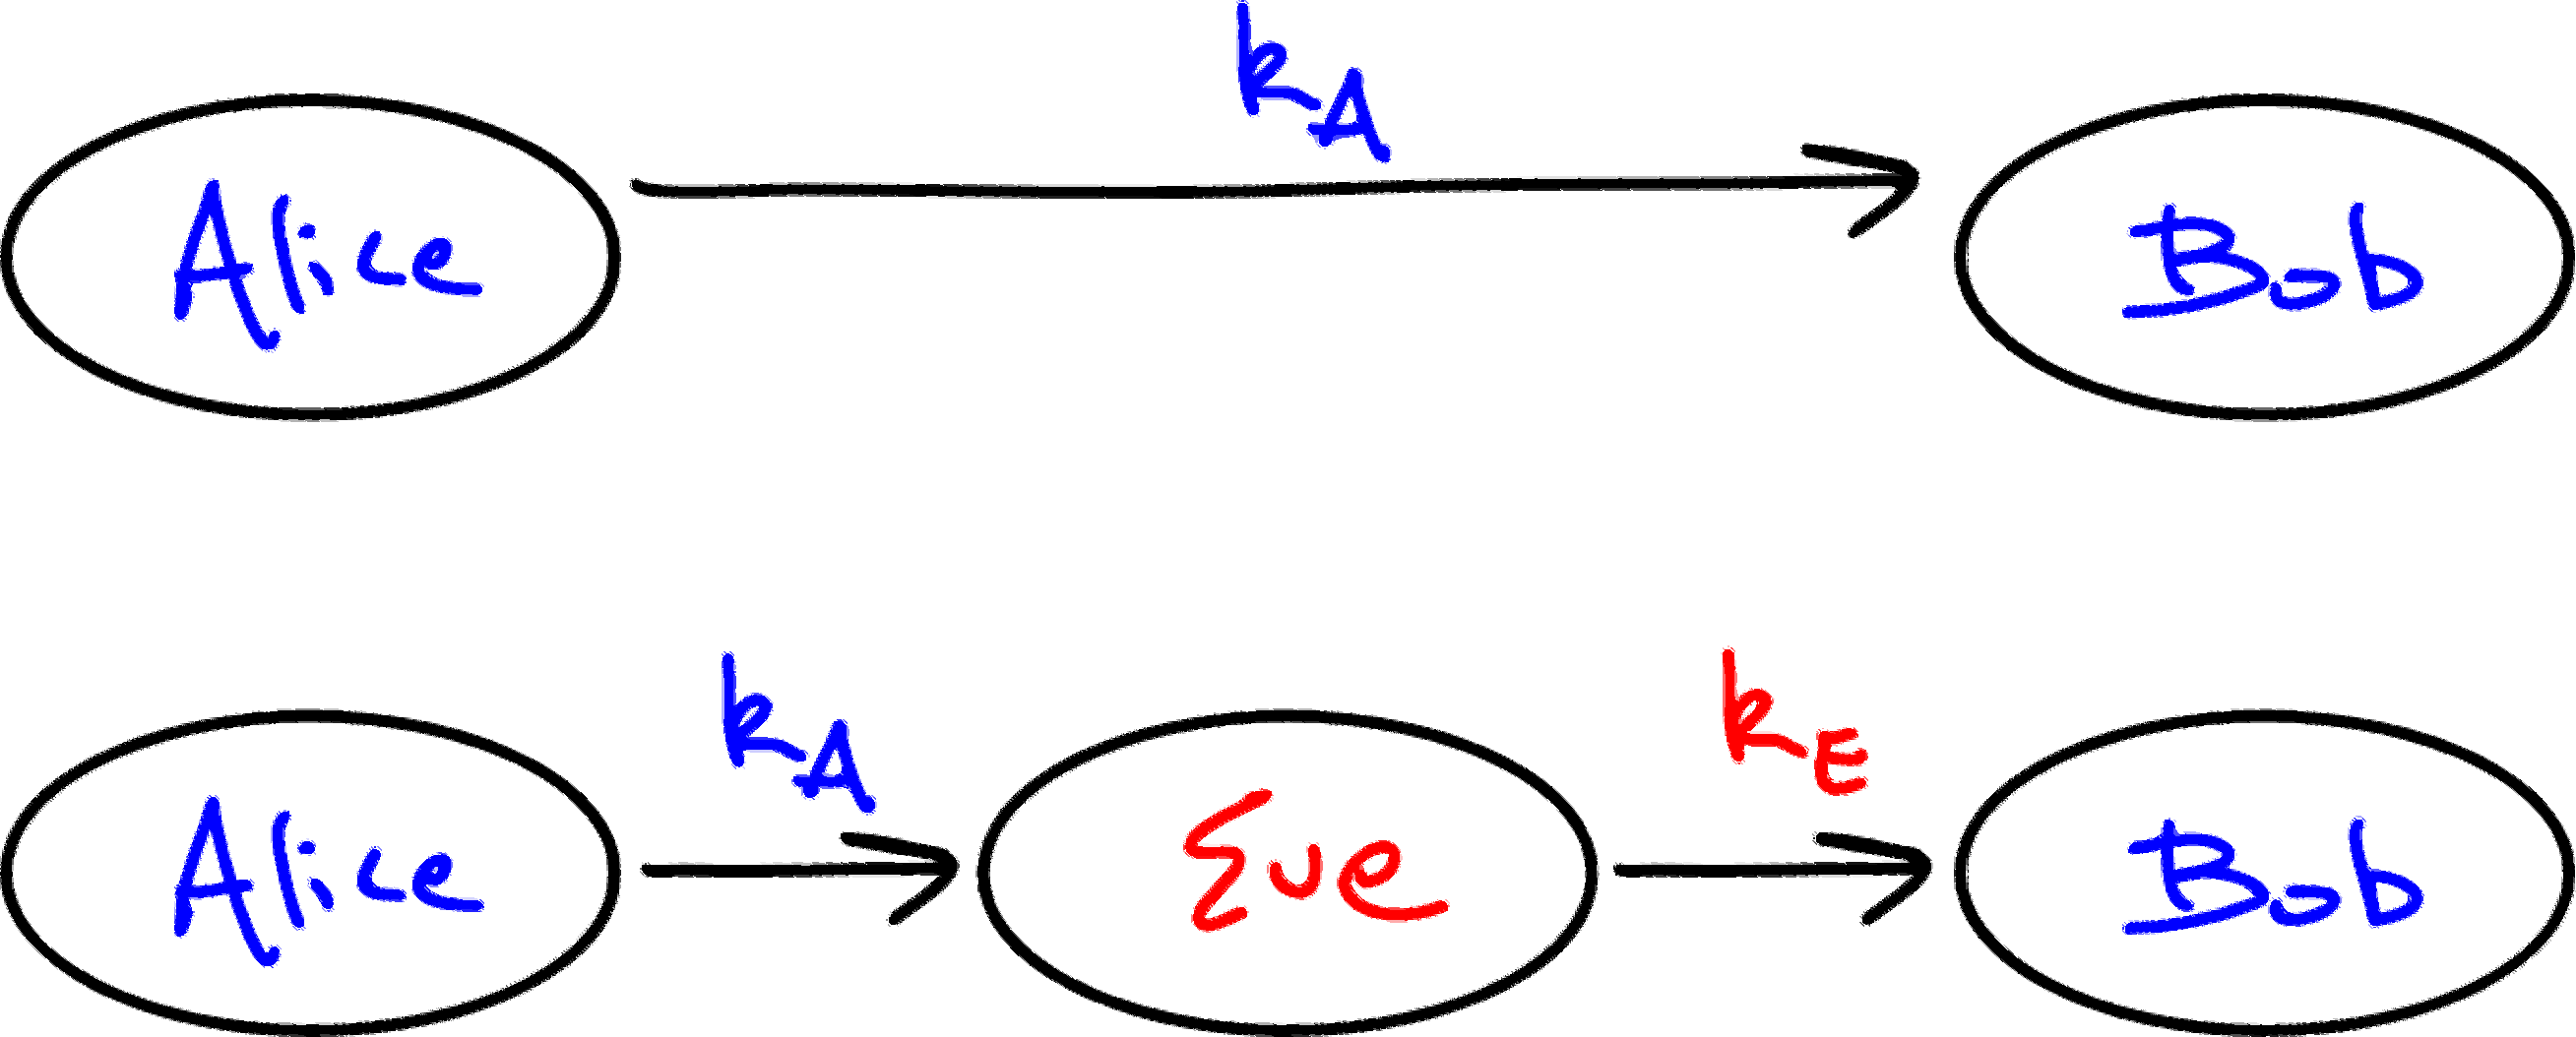
\includegraphics[width=\columnwidth]{figures/Intercept_resend_1}
	\caption{One-way intercept resend-attack. The eveasdropper Eve intercepts Alice's key, retransmitting her own to Bob, spoofing Bob into thinking she is Alice.} \label{fig:MIM_1}
\end{figure}

\begin{figure}[!htb]
	\centering
	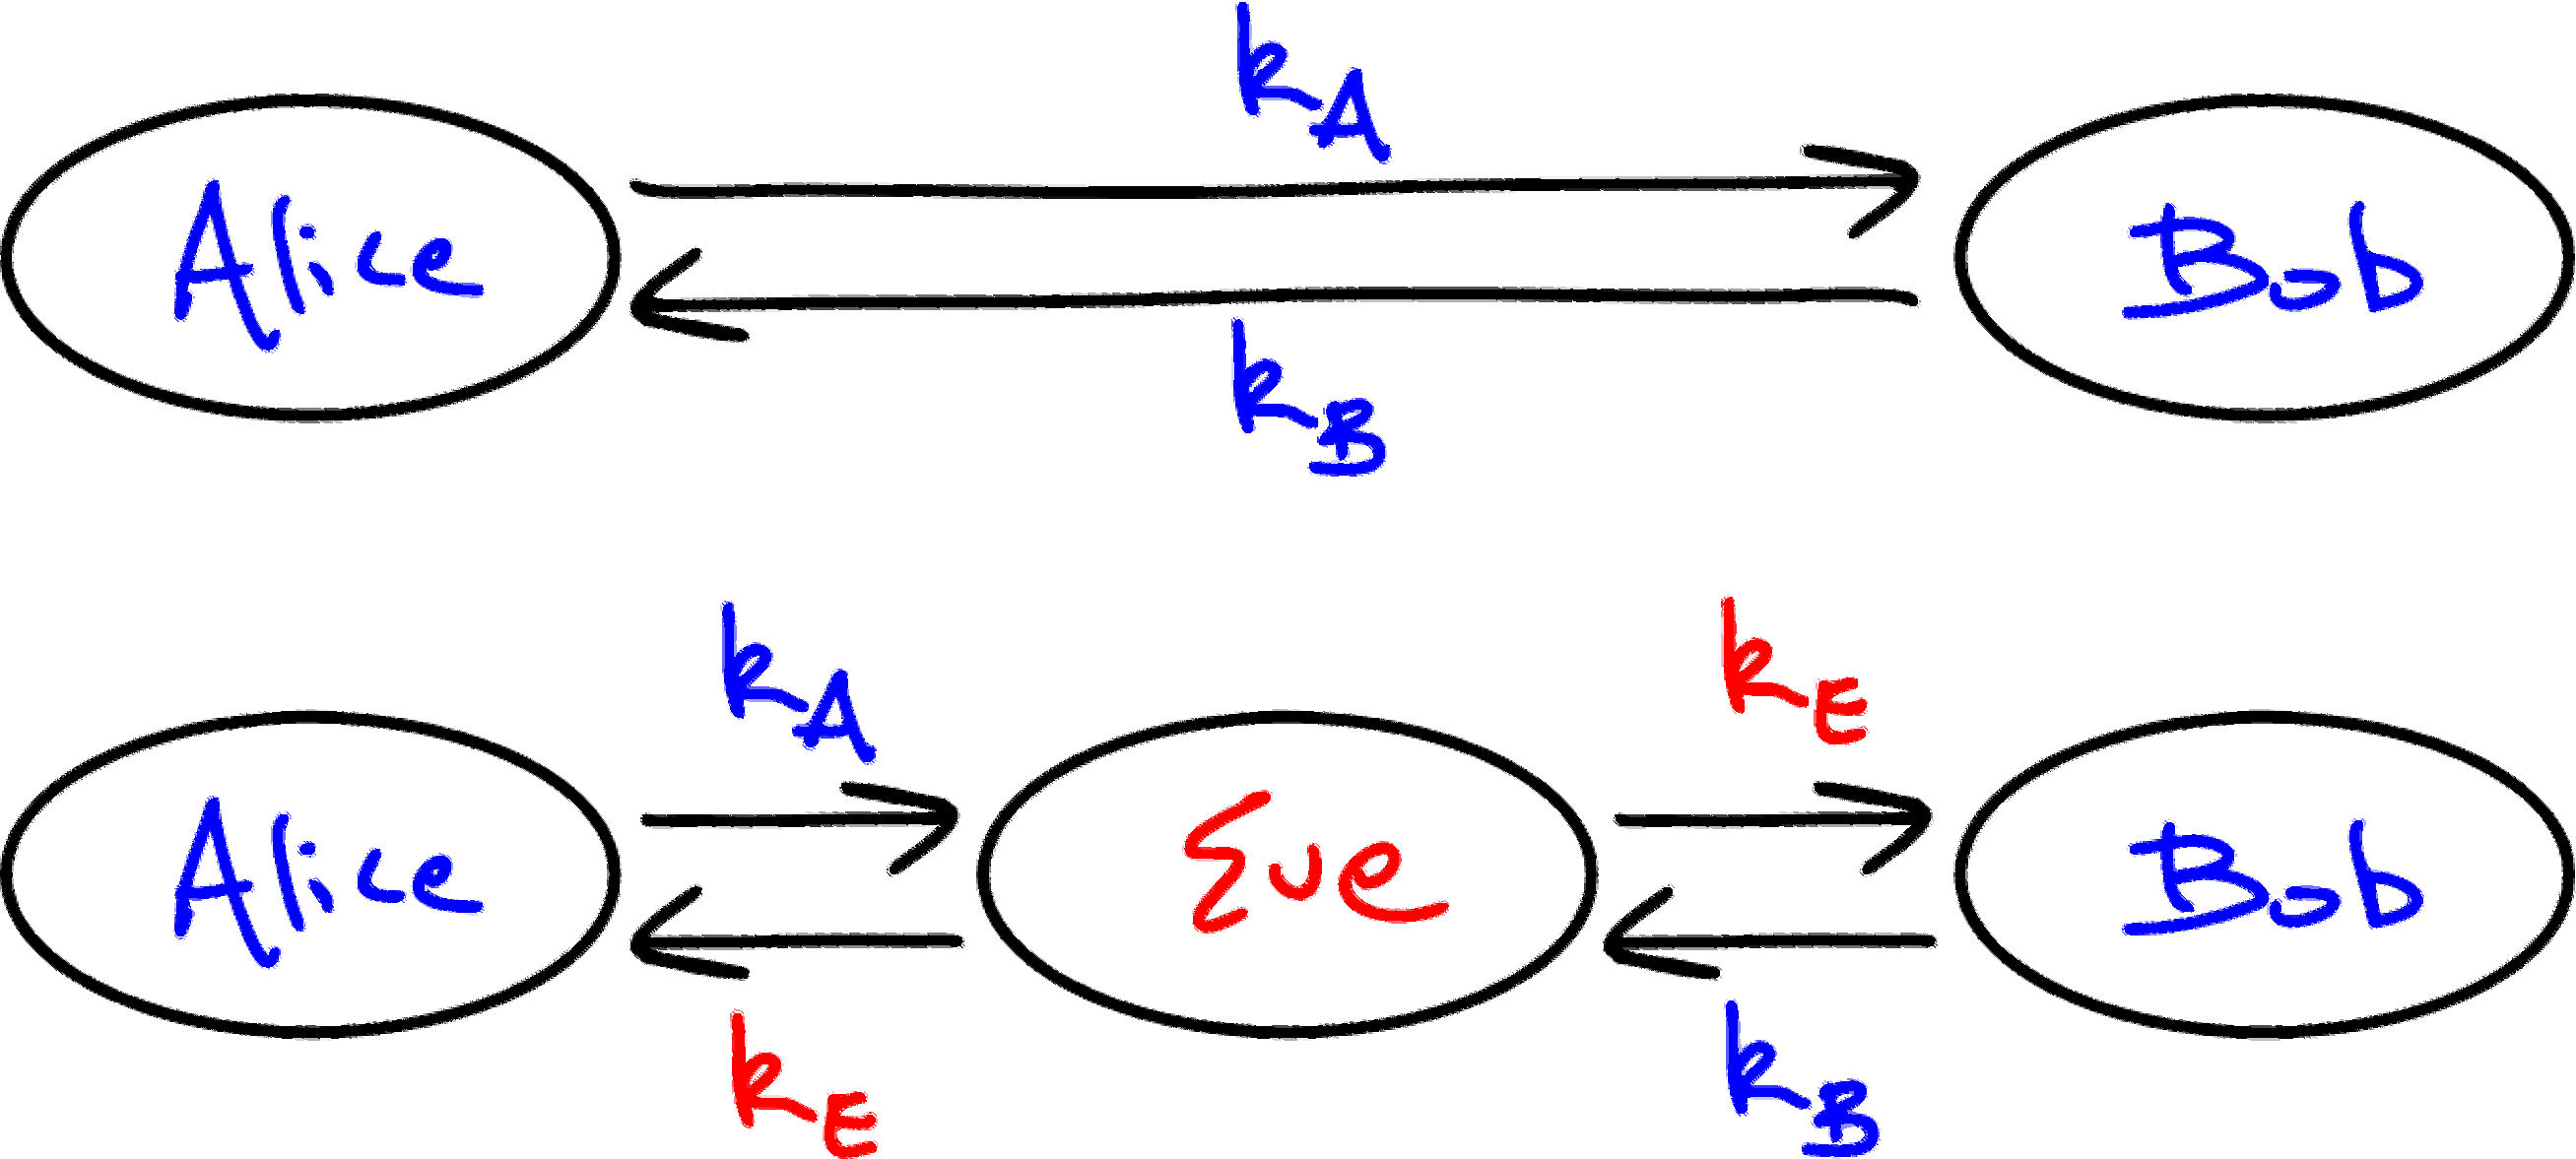
\includegraphics[width=\columnwidth]{figures/Intercept_resend_2}
	\caption{A two-way intercept-resend attack operates the same way as a one-way intercept-resend attack, except in both directions simultaneously, spoofing both Alice and Bob into thinking that she is the other.} \label{fig:MIM_2}
\end{figure}

The only way to truly eliminate man-in-the-middle attacks is for the two parties to have some way of identifying the other. This could be in the form of confidently knowing their public key or having a shared secret key for authentication. In either case, this requires having some trusted means of establishing the authenticity of the authenticating key. For two parties who have never met this becomes logistically tricky, especially in a globalised environment.

\subsubsection{Signature fingerprints}

The Signal messaging app attempts to mitigate this issue by periodically asking users to compare \emph{safety numbers} (see Fig.~\ref{fig:safety_num}), which are just a fingerprint of both parties' public keys,
\begin{align}
	\texttt{fingerprint}_{A,B} = \texttt{hash}(\texttt{hash}(\mathrm{pub}_A)\oplus\texttt{hash}(\mathrm{pub}_B)).
\end{align}

If the safety numbers match it implies they are both using the correct public keys, thereby ruling out a man-in-the-middle. However for this comparison to be meaningful it must take place via an alternate channel that is not likely to be simultaneously compromised by the same man-in-the-middle. For example, users could meet in person to compare numbers (or simply scan the associated QR codes). With slightly less security they could share it via a different digital channel, or by a voice/video call which is hard for a man-in-the-middle to mimic.

\begin{figure}[!htb]
	\centering
	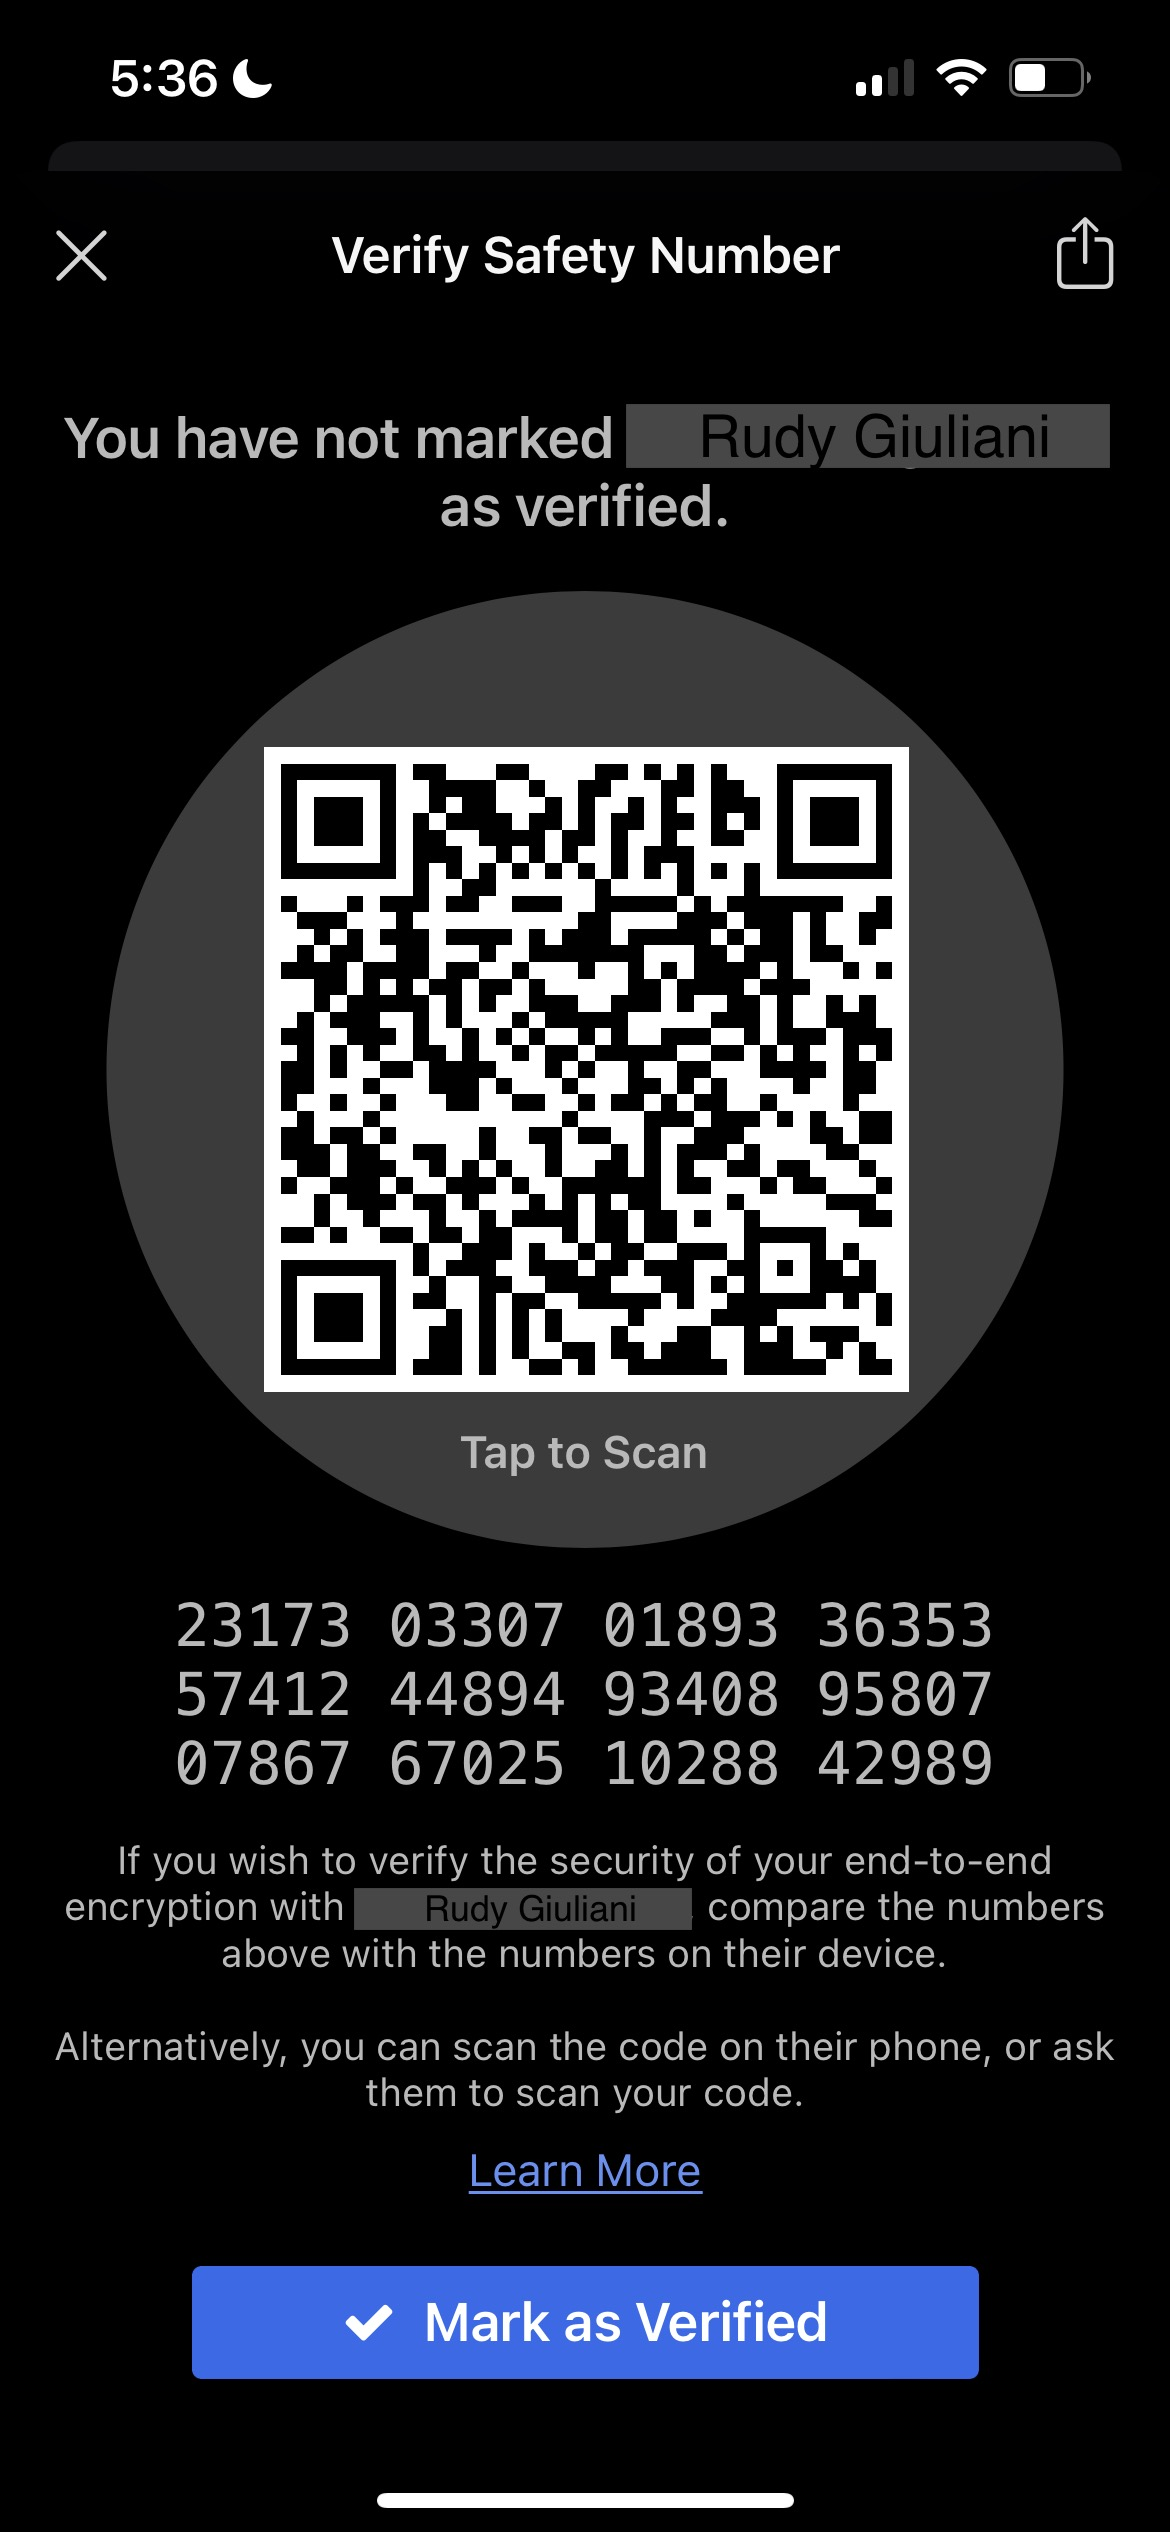
\includegraphics[width=0.8\columnwidth]{figures/Safety_number.jpeg}
	\caption{Safety numbers in the Signal messaging app provide a fingerprint of the users' public keys. When compared via a trusted channel, which needn't be secret, this provides confirmation that the two parties are using one another's public keys, thereby ruling out a man-in-the-middle attack.} \label{fig:safety_num}
\end{figure}

\subsubsection{Certificate authorities} \label{certificate-authorities}

While the previous approach of manually comparing fingerprints might be practical for a messaging app, it isn't viable for more general communications systems, especially ones that communicate with parties they have not previously interacted with, i.e much of the internet.

If we're to rely on public-key cryptography, whether for encryption or digital signatures, how can we ensure the other party actually is who we think it is and isn't being spoofed? How do we know the published public-key we obtained is actually theirs? There are two approaches here:
\begin{enumerate}
\item The public-key is securely shared, requiring some form of secret communication. This somewhat bypasses the whole point of public-key cryptography, which is to avoid the need for secret communication, in which case we'd might as well use private-key cryptography, which is far more robust against quantum attack vectors.
\item We rely on trusted third parties to act as guarantors to vouch for the integrity of the public-keys of others, so-called \emph{certificate authorities}.
\end{enumerate}
%The answer is that somewhere along the line we need to rely on trusted third parties who act as guarantors of the validity of the public keys of others. These trusted third parties are often called \emph{certificate authorities}, who we outsource the hard work of establishing the authenticity of others to.

The latter is the most practical and commonplace method to achieve this (see Fig.~\ref{fig:certificate}). However, since this model relies on trust, it introduces a point of failure -- how do we ensure that the certificate authority itself isn't being spoofed and hasn't been compromised? At some point along the line we are going to have to rely upon the former approach. That is, no matter who we rely on for obtaining the public-keys of others, at some stage we need secure communication to have a trusted public-key for at least \emph{someone}.

For this reason, when you purchase a new computer or mobile phone the pre-installed operating system will have the public-keys of some trusted agencies, such as Apple, Google and/or some other certificate authorities, hard-coded to address this problem. This means spoofing these trusted agencies would require compromising physical devices prior to being sold, a challenging endeavour.

\begin{figure}[!htb]
	\centering
	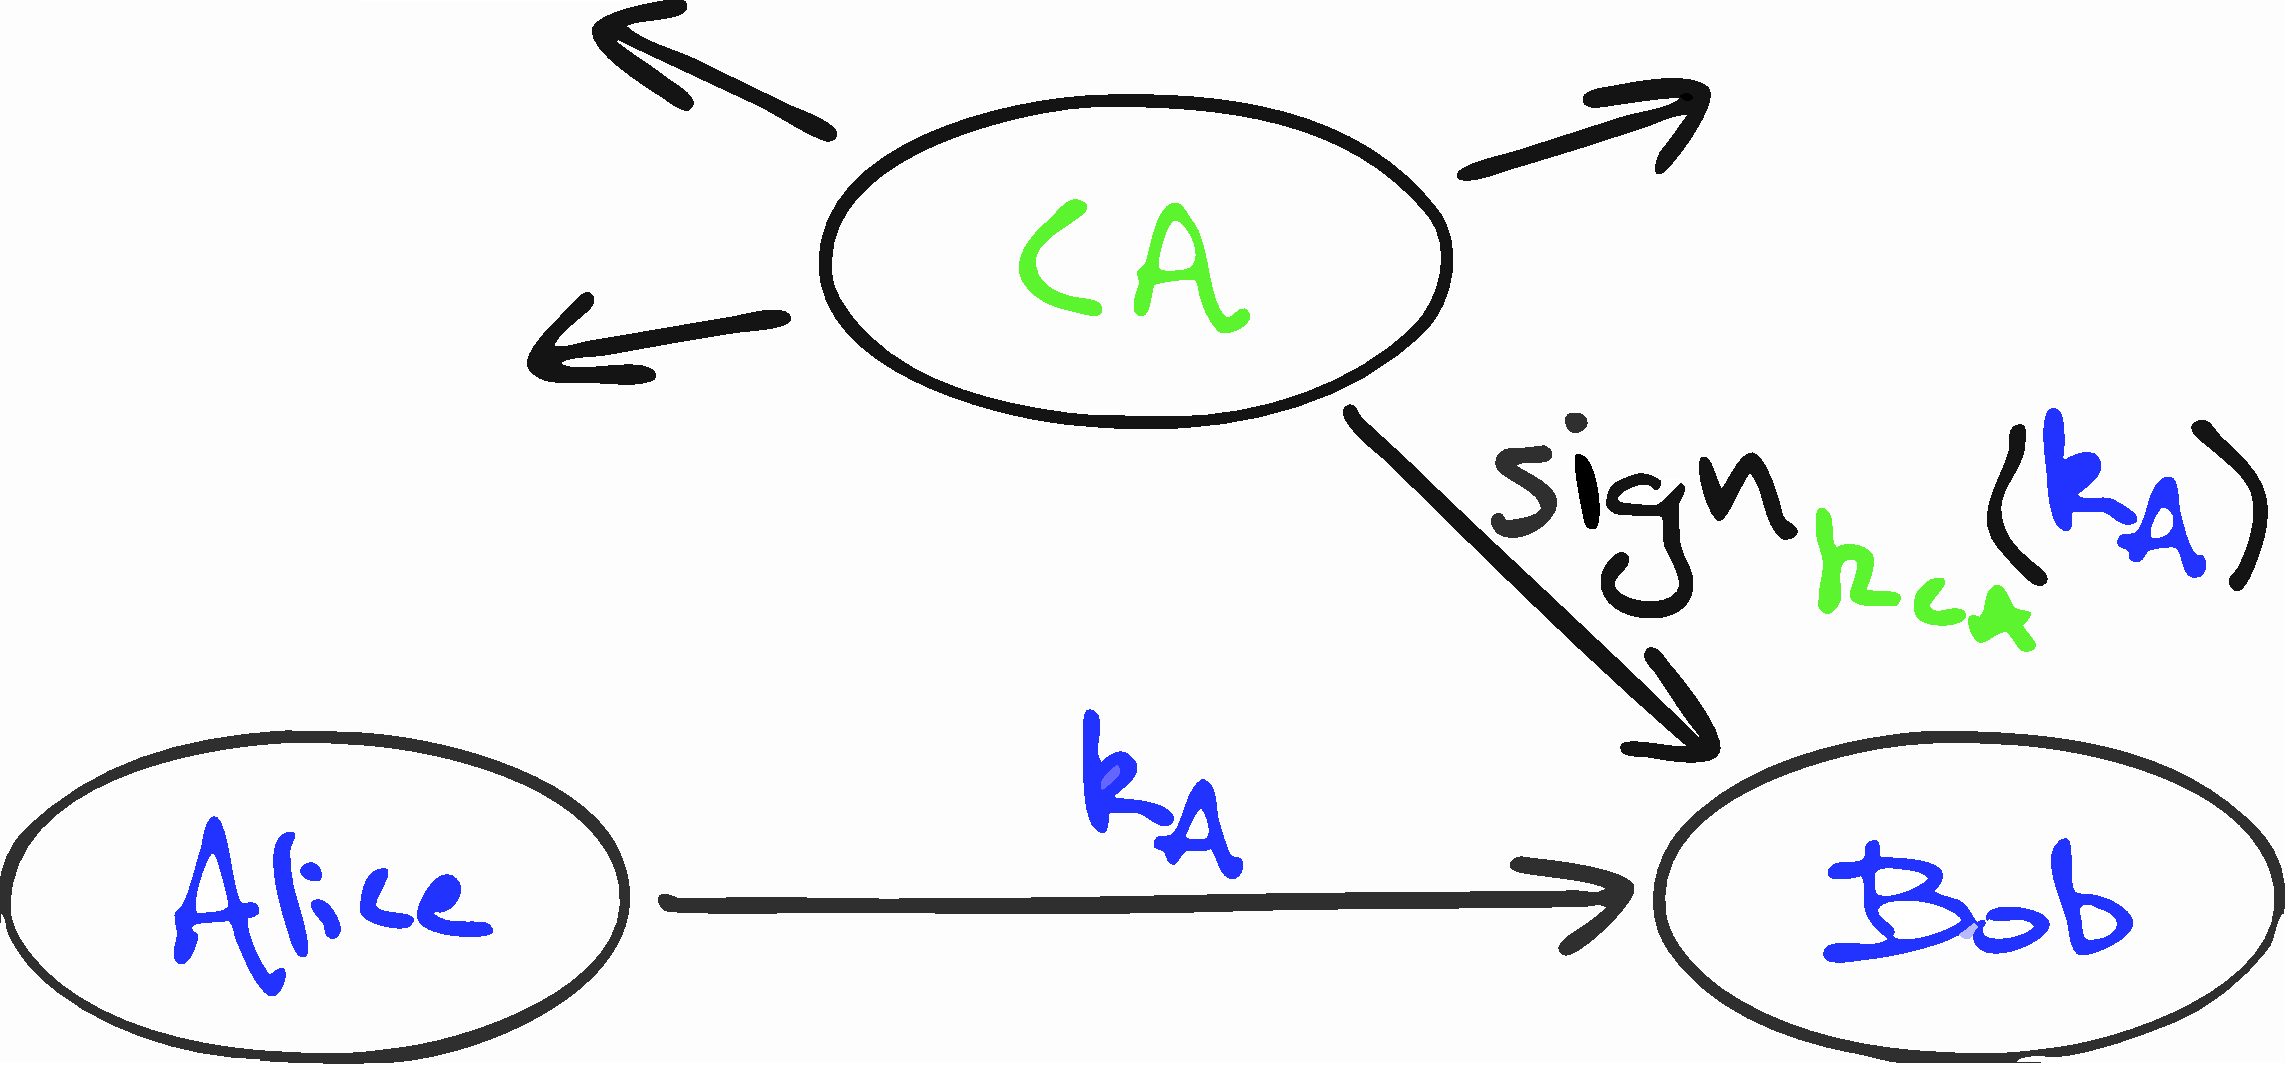
\includegraphics[width=\columnwidth]{figures/Certificate_authority}
	\caption{A certificate authority is a central, trusted agency who signs off on the public keys of other parties, confirming their authenticity. This helps reduce the risk of man-in-the-middle attacks inserting themselves between unknown parties and spoofing them. Here, Alice communicates her public key, $k_A$, to Bob to allow him to securely communicate with her. Bob can't be sure that an eavesdropper Eve isn't inserting herself in between and spoofing Alice, so he queries the trusted certificate authority (CA) who signs Alice's signature to vouch for its integrity, $\mathtt{sign}_{k_{CA}}(k_A)$. Now if Eve is to successfully spoof Alice, she must also compromise or spoof the certificate authority.} \label{fig:certificate}
\end{figure}
\section{Quantum attack vectors} \label{quantum-attack-vectors}

Quantum attacks refer to attack vectors enhanced by quantum resources, which here we'll refer to as being quantum computational resources.

\subsection{Shor's algorithm} \label{shors-algorithm}

The primary vulnerability current public-key cryptosystems have to quantum attack is via Shor's algorithm for integer factorisation \cite{bib:ShorFactor}. This algorithm has time complexity,
\begin{align}
	O((\log n)^2(\log\log n)(\log\log\log n)),
\end{align}
for an integer of size $n$, and therefore resides in \textbf{BQP} with polynomial quantum time complexity. The quantum circuit implementing Shor's algorithm is shown in Fig.~\ref{fig:shor}.

Recall that the best-known classical algorithm for solving this problem, the general number field Sieve, has time complexity,
\begin{align}
	O(e^{c (\log n)^{1/3}(\log\log n)^{2/3}}),
\end{align}
which is classically inefficient.

A variant of Shor's algorithm can also be used to efficiently solve the discrete logarithm problem, making ECC similarly vulnerable to quantum attack. This arises because, while seemingly very distinct, integer factorisation and the discrete logarithm problem are both closely mathematically related to the problem of period finding.

\begin{figure}[!htb]
\centering
\[
	\Qcircuit @C=.5em @R=.5em {
  \lstick{\ket{0}}    & \gate{H} & \qw & \qw               & \qw               & \qw & \cdots & & \ctrl{4}               & \multigate{3}{\textrm{QFT}_{2n}^{-1}} & \qw  & \meter & \cw \\
  \lstick{\vdots\ \ } & \vdots   &     &                   &                   &     &        & &                        &    \pureghost{\textrm{QFT}_{2n}^{-1}} &      & \vdots &     \\
  \lstick{\ket{0}}    & \gate{H} & \qw & \qw               & \ctrl{2}          & \qw & \cdots & & \qw                    &        \ghost{\textrm{QFT}_{2n}^{-1}} & \qw  & \meter & \cw \\
  \lstick{\ket{0}}    & \gate{H} & \qw & \ctrl{1}          & \qw               & \qw & \cdots & & \qw                    &        \ghost{\textrm{QFT}_{2n}^{-1}} & \qw  & \meter & \cw \\
  \lstick{\ket{1}}    & /^n \qw  & \qw & \gate{U{a^{2^0}}} & \gate{U{a^{2^1}}} & \qw & \cdots & & \gate{U{a^{2^{2n-1}}}} & \qw
 }
 \]
 \caption{Quantum circuit for Shor's algorithm.} \label{fig:shor}
\end{figure}

\subsubsection{How fast is Shor's algorithm in practice?} \label{how-fast-is-shors-algorithm-in-practice}

There is the widely held misconception, often repeated in the mainstream media, that quantum computers could spontaneously crack public key encryption, thereby compromising virtually everything on the internet. In reality, although a Shor-armed quantum computer could `efficiently' crack RSA/ECC cryptography (in the computer scientist's sense of the word `efficient'), it would still take considerable time.

The quantum circuit itself for implementing Shor's algorithm is, despite being efficient, very complex, comprising a large number of quantum gates for realistic problem instances, and requiring elaborate error-correction codes to enable fault-tolerance, inducing significant additional overheads.

(??? Steal figures and results from Brennan/Tomamichel)

\subsection{Grover's algorithm}\label{grovers-algorithm}

Grover's algorithm \cite{bib:Grover96} is a quantum algorithm for speeding up \emph{satisfiability problems}. Suppose we have an arbitrary binary circuit with $n$ input bits and a single output bit, and our goal is to find an input bitstring that evaluates to 1 at the output. We say that the corresponding input is a \emph{satisfying input}. Next, suppose there is only one satisfying input and our goal is to find it (see Fig.~\ref{fig:SAT}).

Classically, without knowing anything about the structure of the circuit, the best we could do is exhaustively search the input space, of which there are $2^n$ combinations. This is referred to as an \emph{unstructured search problem}. The classical runtime, therefore, scales as $O(2^n)$.

Grover's algorithm (ignoring any architectural or fault-tolerance overheads) provides a quadratic enhancement to this, yielding a quantum runtime of only,
\begin{align}
    O(\sqrt{2^n}) = O(2^{n/2}).
\end{align}
The circuit implementing Grover's algorithm is shown in Fig.~\ref{fig:grover}.

\begin{figure*}[!htb]
	\centering
	\[]
	 \Qcircuit @C=1em @R=.7em {
                   &         &                      &                         &                      & \ustick{\text{Grover diffusion operator}} \\
  \lstick{\ket{0}} & /^n \qw & \gate{H^{\otimes n}} & \multigate{1}{U_\omega} & \gate{H^{\otimes n}} & \gate{2 \ket{0^n}\bra{0^n} - I_n}         & \gate{H^{\otimes n}} & \qw & \cdots & & \meter & \cw \\
  \lstick{\ket{1}} & \qw     & \gate{H}             & \ghost{U_\omega}        & \qw                  & \qw                                       & \qw                  & \qw & \cdots & \\
                   &         &                      &                         &                      & \dstick{\text{Repeat $O(\sqrt{N})$ times}}
  \gategroup{2}{5}{2}{7}{.7em}{^\}}
  \gategroup{2}{4}{3}{10}{.7em}{_\}}
 }
 \]
\caption{Quantum circuit for Grover's algorithm.} \label{fig:grover}	
\end{figure*}

We see that Grover's algorithm does \emph{not} provide an exponential quantum speedup, only a quadratic one. From a runtime perspective, this means Grover's algorithm effectively halves the size of the input bit-string.

\begin{figure}[!htb]
	\centering
	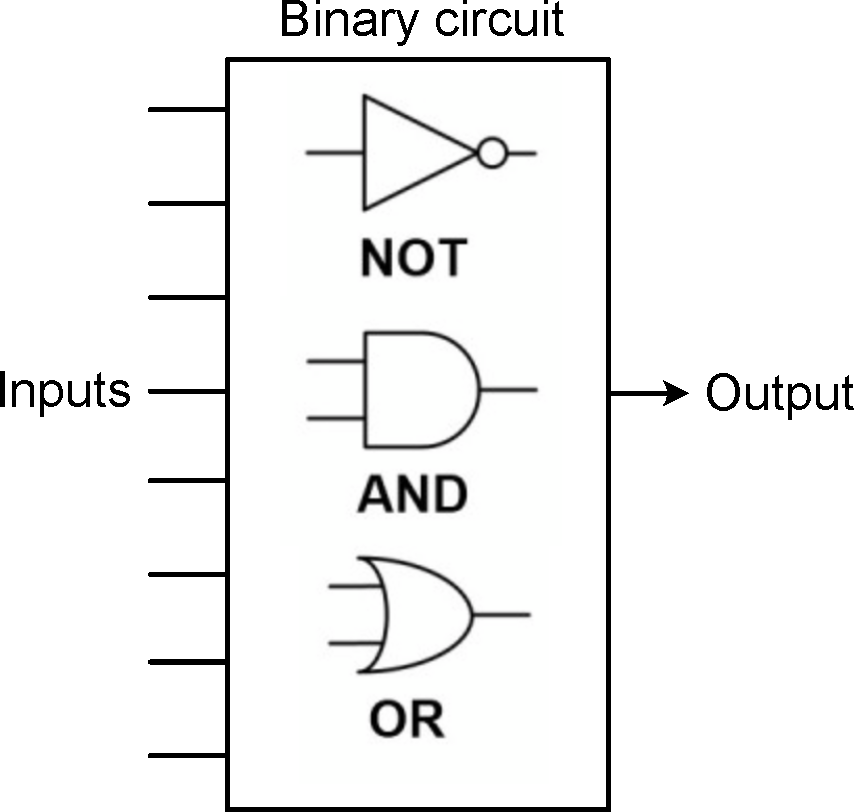
\includegraphics[width=0.7\columnwidth]{figures/SAT}
	\caption{A binary satisfiability problem. A circuit comprising universal binary logic gates (e.g AND, OR and NOT) is applied to an arbitrarily sized input to yield a single output bit. The goal is to find a `satisfying input' such that the respective output yields a 1.} \label{fig:SAT}
\end{figure}

Breaking \emph{any} encryption scheme, private or public, can be viewed as a satisfiability problem, where we ask the satisfiability question ``What key decrypts this ciphertext to something sensible?''. The exception to this is the one-time-pad, since there are keys that decrypt any given message to \emph{every} possible plaintext of the same length, all of which meet the satisfiability criteria.

Similarly, inverse hashing also takes the form of a satisfiability problem, where we want to find an input that maps to a given output. Using Grover's algorithm inverse hashing remains an exponentially hard problem on quantum computers, just a quadratically reduced exponential.

In the quantum era it will therefore be diligent to use private keys and cryptographic hashes of twice the length of what is presently considered secure in order to maintain the same level of security. These are relatively straightforward transitions to make, but ones worth considering implementing today for information with forward value.

\subsection{Symmetric ciphers} 

???

Some, but not all, symmetric ciphers are also vulnerable to efficient quantum attacks via Simon's period finding algorithm. Simon's problem can be stated as follows. For a binary function,
\begin{align}
f: \{0,1\}^n \to \{0,1\}^n,
\end{align}
which satisfies,
\begin{align}
f(x) = f(x\oplus s)	
\end{align}
for some value of $s$ (not including the trivial case where $s=0^n$), where $x,s\in \{0,1\}^n$, the goal is to determine $s$ by querying $f(x)$. Here, $s$ is referred to as the \emph{period} of the function.

The best classical algorithm for solving this problem requires $O(\sqrt{2^n})$ queries, whereas Simon's quantum algorithm requires only $O(n)$ queries, providing an exponential separation between Simon's algorithm and the best classical algorithm. The quantum circuit implementing Simon's algorithm is shown in Fig.~\ref{fig:simons}.

\cite{bib:kaplan2016breaking}

% https://link.springer.com/content/pdf/10.1007/978-3-662-53008-5_8.pdf
% https://en.wikipedia.org/wiki/Slide_attack

\begin{figure}[!htb]
\centering
\[
 \Qcircuit @C=1em @R=.7em {
  \lstick{\ket{0}} & /^n \qw & \gate{H^{\otimes n}} & \multigate{1}{U_f} & \gate{H^{\otimes n}} & \meter & \cw \\
  \lstick{\ket{0}} & /^n \qw & \qw                  & \ghost{U_f}        & \qw                  & \meter & \cw
  }
 \]
 \caption{Quantum circuit for Simon's algorithm.} \label{fig:simons}
\end{figure}
\section{Quantum cryptography} \label{quantum-cryptography}

In Sec.~\ref{classical-cryptography} we introduced a number of important classical cryptographic primitives. We now do the same in the context of quantum hardware.

\subsection{Quantum random number generation (QRNG)} \label{quantum-random-number-generation-qrng}

Randomness is an important cryptographic primitive, most notably when used for key generation. Most commonly, the randomness generated by classical computers is actually pseudo-randomness. That is, it is generated via a deterministic algorithm that takes various input data sources, like the current time and various hard-to-predict parameters from the system (or \emph{seed}) from which a bit-stream is generated that is sufficiently hard to predict that it is considered `good enough to be considered random'. These pseudo-random number generation algorithms qualitatively have a lot in common with cryptographic hash functions. Indeed hash functions could be directly employed for this purpose.

However this `good enough to be considered random' criteria has on occasion failed us quite spectacularly (??? refs), exposing cryptosystems to significant vulnerabilities.

It would be far better if we could eliminate the term `pseudo' altogether and have true randomness, with no hidden patterns or correlations. In a deterministic world, as described by Newtonian physics one would correctly argue this is not possible. However quantum mechanics, via Heisenberg's uncertainty principle, provides avenues for generating true randomness.

Consider a photon in an equal superposition of the two polarisation states,
\begin{align}
	|+\rangle=\frac{1}{\sqrt{2}}(|H\rangle+|V\rangle).
\end{align}
Now upon measuring in the horizontal/vertical basis we measure each polarisation outcome with probability of 1/2 since,
\begin{align}
	|\langle H|+\rangle|^2 &= \frac{1}{2},\nonumber\\
	|\langle V|+\rangle|^2 &= \frac{1}{2}
\end{align}
This probability refers to genuine randomness, unlike pseudo-randomness which is a hidden variable approach whereby not knowing the internal state of the random number generator is what prevents us from predicting its output. The measurement collapse effect in quantum mechanics is provably \emph{not} a consequence of such a hidden variable theory, as famously shown by John Bell \cite{bib:bells-theorem}.

It isn't hard to see that QRNG lies on the easy end of quantum engineering, and indeed numerous commercial providers sell QRNG units as off-the-shelf products today. A simple implementation could be constructed from a photon source, polarization filter, polarising beamsplitter and two photo-detectors (see Fig.~\ref{fig:QRNG}).

\begin{figure}[!htb]
	\centering
	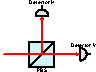
\includegraphics[width=0.7\columnwidth]{figures/QRNG.pdf}
	\caption{A simple implementation of a quantum random number generator. A single photon source is filtered to yield a stream of photons with $45^\circ$ diagonal polarisation. These pass through a polarising beamsplitter, which transmits vertically polarised photons and reflects horizontally polarised ones. The diagonally polarised photons have 50/50 likelihood of triggering each of the detectors, yielding a binary stream of random bits.} \label{fig:QRNG}
\end{figure}

\subsection{Quantum key distribution (QKD)} \label{quantum-key-distribution-qkd}

??? hybrid with AES

In Sec.~\ref{one-time-pad-encryption} we introduced the one-time-pad cipher, the only provably (i.e information theoretically) secure classical encryption technique. However, despite its perfect security it was deemed highly impractical due to the need to continually establish new secret keys because they can't be reused.

Quantum key distribution (QKD) refers to a set of quantum protocols for securely sharing random bit-strings between parties. These could subsequently be used in any symmetric cipher, including the Holy Grail of the one-time-pad.

\subsubsection{BB84} \label{bb84}

The BB84 protocol (named after its inventors and the year of invention) \cite{bib:bb84} uses single photons to encode qubits used to share secret random bit-strings between end-users for use in a one-time-pad or other symmetric cipher (see Fig.~\ref{fig:BB84}).

We begin by defining two bases in which to encode a qubit with logical value 0 or 1 into the polarisation of a photon. The first is the horizontal/vertical basis:
\begin{align}
	|0\rangle &= |H\rangle,\nonumber\\
	|1\rangle &= |V\rangle.
\end{align}
The second is the diagonal/anti-diagonal basis (i.e a 45-degree polarization rotation compared to the first case): 
\begin{align}
	|0\rangle &= |D\rangle = \frac{1}{\sqrt{2}}(|H\rangle+|V\rangle),\nonumber\\
	|1\rangle &= |A\rangle = \frac{1}{\sqrt{2}}(|H\rangle-|V\rangle).
\end{align}
We now observe that if a qubit is measured in the same basis in which it is encoded we will necessarily recover the correct qubit value. If, on the other hand, we measure in the wrong basis, we get a random value (as per the quantum random number generator in Sec.~\ref{quantum-random-number-generation-qrng}).

Next Alice randomly chooses values to encode into her qubits (0 or 1), and also randomly chooses which bases to encode them in ($H$/$V$ or $D$/$A$). She sends a stream of such randomly encoded qubits to Bob. Bob now measures all the qubits in randomly chosen bases. The ones where by chance he measures in the basis Alice encoded in, they are guaranteed to share the result. If not, then not.

Alice then (publicly) announces which bases she encoded in, but not what the encoded values were (they are the secret). Bob similarly publicly announces which bases he measured in. They then filter their results to keep only the ones where encoding and measurement bases were consistent, from which they establish a shared random bit-string.

But how do we rule out a man-in-the-middle attack? To do this, Alice and Bob sacrifice some of their shared data and compare it over a public channel. If any inconsistencies are found it implies someone in the middle had intercepted those qubits, measured them, and re-encoded them, but not knowing which random basis to re-encode in, got it wrong. That is, because measurements collapse quantum states, intercept-resend attacks will introduce inconsistencies between the bit-strings of the end-users.

The final stage after sacrificing some shared bits to determine whether a man-in-the-middle attack has taken place is to perform \emph{privacy amplification}. The shared string may still may contain some exposed bits, which is mathematically reduced to a shorter shared string with higher security. This can be made asymptotically strong.

\begin{figure}[!htb]
	\centering
	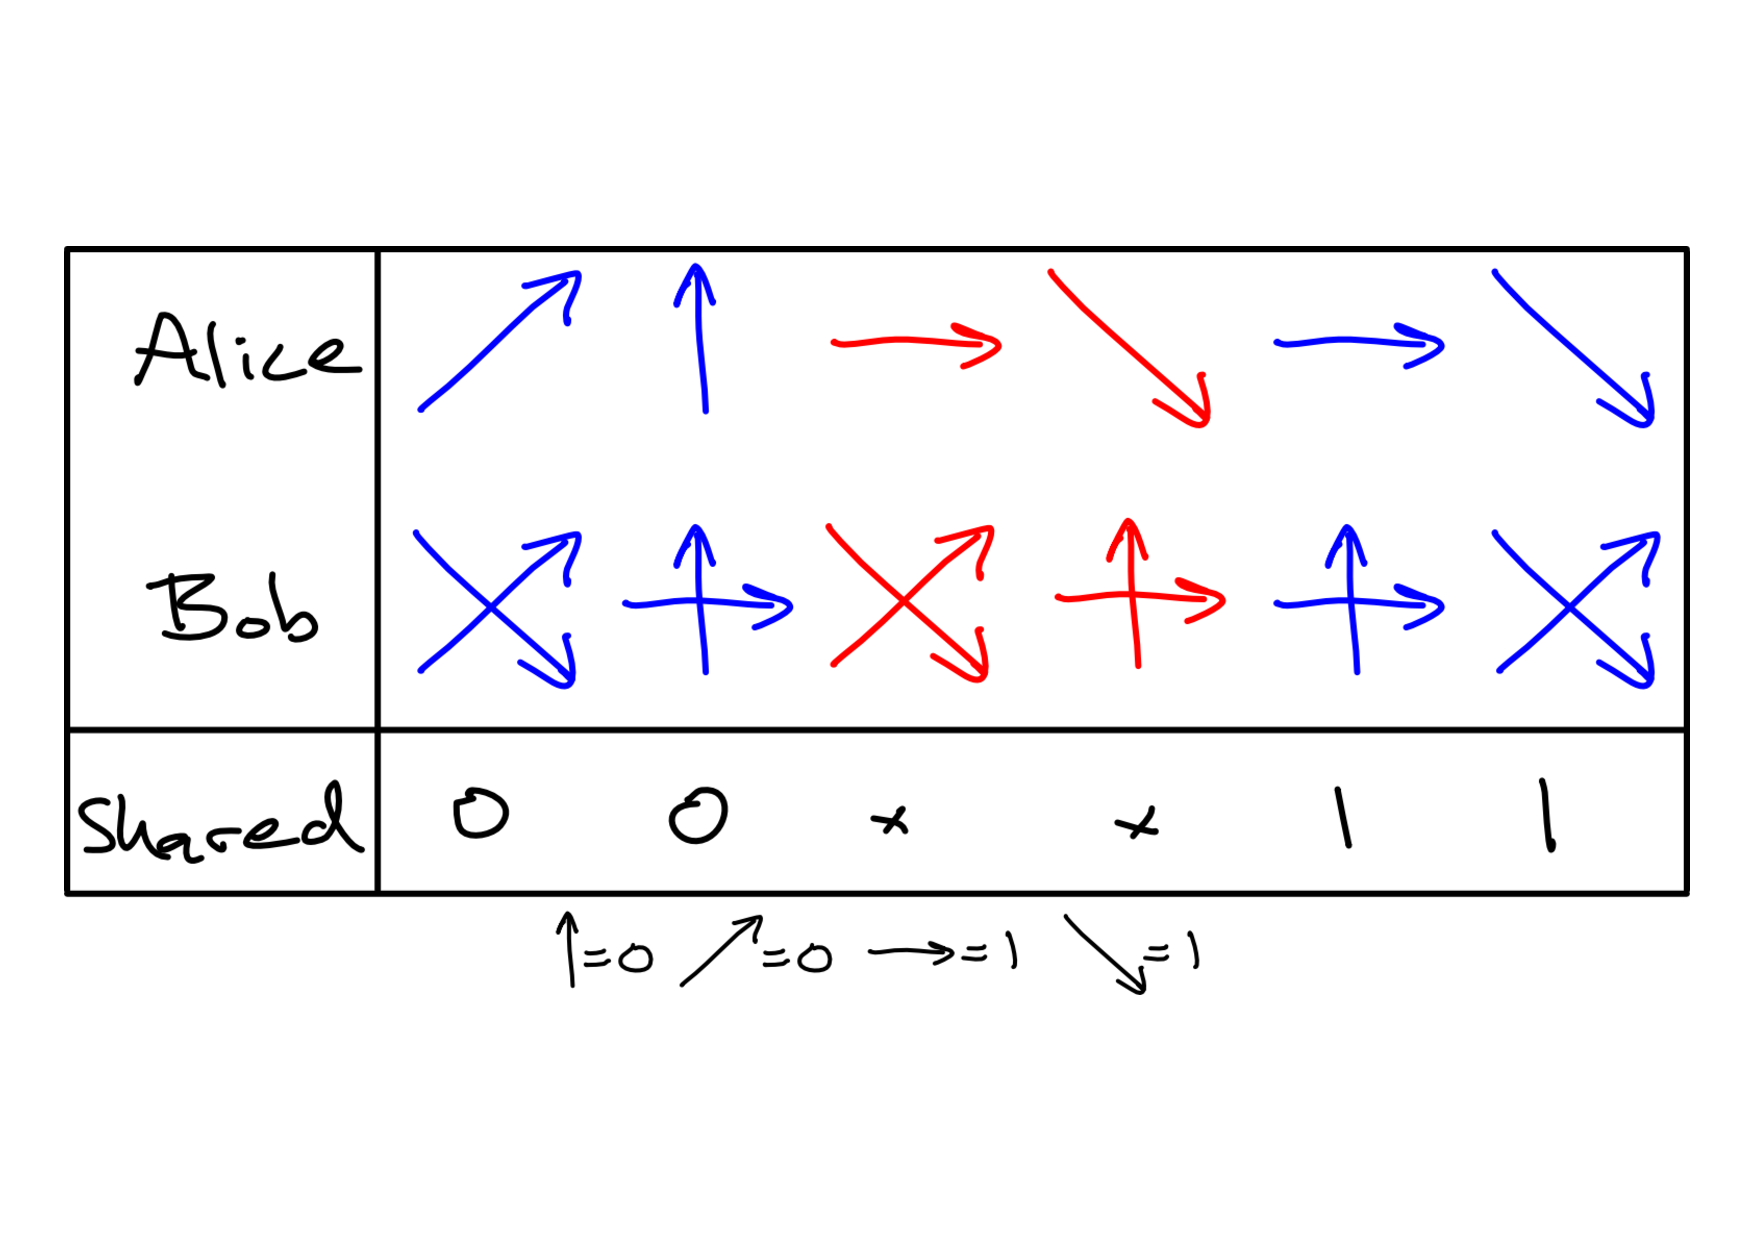
\includegraphics[width=\columnwidth]{figures/BB84}
	\caption{Example encodings and measurements for the BB84 protocol. Upon classical post-processing, Alice and Bob are left with secure, shared randomness that can be employed in a one-time-pad cipher for information-theoretically secure encryption.} \label{fig:BB84}
\end{figure}

\subsubsection{E91} \label{e91}

The so-called E91 protocol (again named after the inventor and year of invention) \cite{bib:ekert1991quantum} makes the same promise and has similar operation to BB84. The difference between BB84 and E91 is that BB84 relies on the communication of single qubits whereas E91 relies upon both parties sharing an entangled Bell pair.

A Bell pair is a maximally entangled, two-qubit state, which can equivalently be written as
\begin{align}
	|\Psi\rangle &= \frac{1}{\sqrt{2}}(|H,H\rangle+|V,V\rangle)\nonumber\\
	&= \frac{1}{\sqrt{2}}(|D,D\rangle+|A,A\rangle),
\end{align}
in the horizontal/vertical and diagonal/anti-diagonal bases respectively. 

With a large number of such shared pairs, for each pair, the operation proceeds similarly to BB84. Alice randomly measures either in the horizontal/vertical basis or diagonal/anti-diagonal basis, after which Bob's state will be identical to her measurement outcome if he measures in the same basis or completely random if he doesn't. Over an unsecured channel, they then compare their measurement \emph{bases} after which the ones where they measured consistently must have been the same. Should someone attempt to perform an intercept-resend attack this will randomise their results resulting in inconsistencies upon sacrificing a subset of their shared bits for comparison, as per BB84.

While the operation and outcome are almost identical, the key difference here is that communicating shared Bell pairs has some practical advantages over communicating single qubits as per BB84. Bell pairs can in principle be communicated over very long distances using quantum repeater networks, which utilise the concepts of entanglement swapping and entanglement purification to overcome the issue that the probability of a single qubit successfully traversing a lossy channel drops exponentially with distance, thereby imposing distance limitations. Quantum repeaters overcome this efficiency problem and could in principle be utilised over extremely long distances in the presence of loss. This is one of the key reasons why a future quantum internet \cite{bib:RohdeQI} will be entanglement-based rather than single-qubit communication-based. Entanglement-based QKD has been demonstrated via satellite over distances $\sim$1,500km (see Fig.~\ref{fig:satellite})

\begin{figure}[!htb]
	\centering
	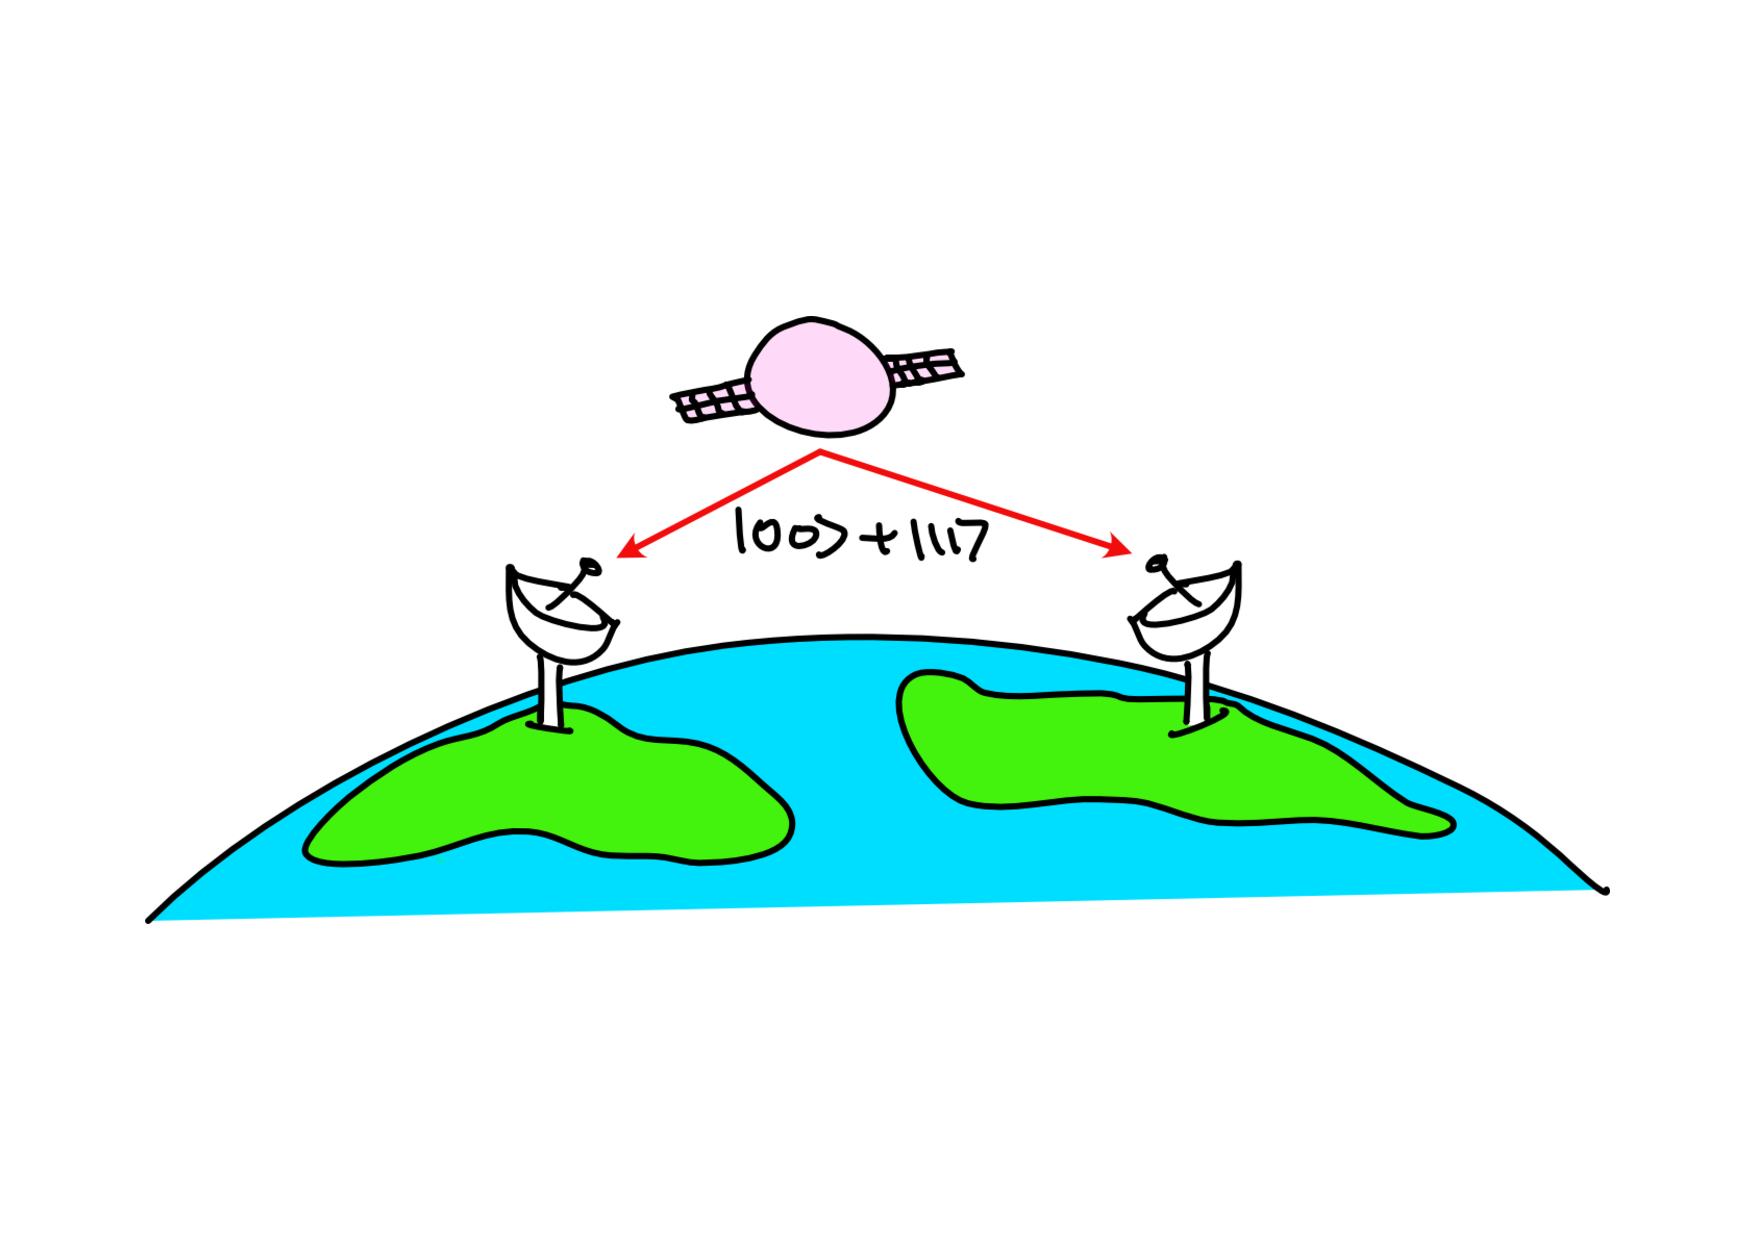
\includegraphics[width=\columnwidth]{figures/Satellite}
	\caption{Space-based entanglement distribution has successfully demonstrated low-bandwidth quantum key distribution over a range of $\sim$1,500km.} \label{fig:satellite}
\end{figure}

\subsubsection{Side-channel attacks} \label{side-channel-attacks-qkd}

While QKD is often quoted as offering \emph{perfect} security, this is far from the truth. QKD offers perfect security in the idealised theoretical setting whereby, in the case of E91 for example, two parties have shared Bell pairs and measure them. However, it is fanciful to think this ideal setting applies once the engineers get involved.

Bell pairs need to be prepared and it isn't as straightforward as it sounds to prepare a perfect Bell pair of the form,
\begin{align}
	|\Psi\rangle = \frac{1}{\sqrt{2}}(|H,H\rangle+|V,V\rangle),
\end{align}
that is exactly that, and nothing more, with no other entanglements or correlations with the environment or anything else. Should the prepared state deviate in any way from the ideal, this has the potential to open up avenues for information to be adversarially extracted. This might happen, for example, if the polarisation state were correlated with some other detectable photonic degree of freedom, or detectable signals emanating from the preparation device.

One type of attack that has previously undermined some QKD systems is the \emph{photon number splitting attack}. This exploits the fact that some photon sources sometimes produce multiple photons when they are only meant to produce one. Spontaneous parametric down-conversion (SPDC) sources, for example, exhibit this characteristic, as per the photon number distribution given in Eq.~\eqref{eq:SPDC_number}. Similarly, if single photon states are approximated using low intensity coherent states\footnote{Coherent states approximate laser light sources.} of the form,
\begin{align}
	\ket\alpha = e^{-\frac{|\alpha|^2}{2}} \sum_{n=0}^\infty \frac{\alpha^n}{\sqrt{n!}}\ket{n},
\end{align}
where $\alpha$ is the coherent amplitude, the photon number distribution is given by,
\begin{align}
	P(n) = e^{-\langle n\rangle}\frac{\langle n\rangle^n}{n!},	
\end{align}
where $\langle n\rangle=|\alpha|^2$ is the mean photon number. Note that higher-order photon-number terms always exists, irrespective of mean photon number $\langle n\rangle$. The likelihood of higher-order terms occurring is given by,
\begin{align}
	P(n>1) = \sum_{n=2}^\infty P(n).
\end{align}
For the case of mean photon number $\langle n\rangle=1$, this yields $P(n>1)\approx 0.264$. If those unwanted photons are correlated with the signal photon, intercepting them by tapping off part of the signal can reveal information to the adversary.

Another type of side-channel attack is \emph{timing attacks}. Consider the BB84 protocol where we randomly encode photonic qubits into different initial values $H$, $V$, $D$ or $A$. Suppose the setup was not perfectly temporally balanced and preparing some states caused them to exhibit a slight time offset compared to others. This could happen, for example, if encoding in different bases were implemented by following different optical paths to route through different polarisation rotation operations. This would effectively correlate the arrival time of photons with their polarisation encoding, whereby an eavesdropper could infer the polarisation state of photons from their detection time, enabling an undetectable intercept-resend attack. Although this particular attack can be mitigated by randomising state preparation times, it provides a conceptual example for just how easy it is for unwanted correlations introduced by imperfect engineering to thwart the in-principle perfect security offered by QKD.

This notion extends more generally to any other non-polarisation degree of freedom. If there exists distinguishing information between photons prepared into different basis states, measuring that degree of freedom reveals the associated polarisation state. Enormous care must be taken in real-world implementations to ensure that no such distinguishing information or unwanted correlations exist.

Similarly, sources, detectors and their control electronics may have detectable signatures of their own. Should an electronic control circuit emit distinct radiation signals upon different detection events taking place, this also provides avenues for side-channel attacks. There has been no shortage of tit-for-tat between QKD experimentalists demonstrating `perfect security' only for a simple exploit to later be discovered. In our minds, the vulnerabilities of QKD to side-channel attacks, which are not nearly as well studied as their classical counterparts, lead us to \emph{not} recommend relying exclusively on QKD for security, instead opting for hybrid approaches if QKD is to be employed (see Sec.~\ref{hybrid-cryptography}).

The other issue, as discussed previously, is that any secure connection requires channel authentication to eliminate eavesdroppers performing man-in-the-middle attacks, thereby making the security of systems only as strong as their channel authentication protocols. This requires either establishing a shared secret via direct means (e.g two spies meeting in person at the Embassy), relying on classical digital signatures, or on trusted third parties to act as guarantors.

\subsubsection{Denial-of-service (DoS) attacks} \label{denial-of-service-dos-attacks}

One very important attack vector especially relevant to QKD is denial-of-service (DoS) attacks. These are not intended to gather secret information, but to deny others the ability to securely communicate. Since QKD infrastructure will likely always be far more expensive and sparse than our classical networks, there will inevitably be less redundancy should links fail, making them far easier to disrupt. Additionally, due to the enormous precision and sensitivity of quantum systems, combined with the fact that broadcasting quantum messages is not possible, instead requiring point-to-point communication, such disruption is relatively easy compared to classical systems which are far more versatile and robust.

\subsection{Satellite-based QKD} \label{satellite-qkd}

China's satellite for entanglement distribution is one of the most impressive engineering achievements in our field in recent years, allowing Bell pairs to be shared across a distance of over 1,500km. The satellite contains a spontaneous parametric down-converter (SPDC) entanglement source, the most readily available type of entanglement source. Using this satellite Chinese researchers were able to demonstrate QKD over extremely long distances. It is worth commenting on the future prospects of this method of entanglement distribution.

The SPDC source produces states of the form,
\begin{align} \label{eq:SPDC}
	\ket\psi_\mathrm{SPDC} = \sqrt{1-\chi^2}\sum_{n=0}^\infty \chi^n \ket{n,n},
\end{align}
where $|\chi|<1$ characterises the pump power. That is, in the photon-number degree of freedom they exhibit a photon-number distribution of,
\begin{align} \label{eq:SPDC_number}
P(n) = (1-\chi^2)\chi^{2n},
\end{align}
following a power-law with mean photon number,
\begin{align}
	\langle n \rangle &= \sum_{n=0}^\infty P(n) \cdot n = \frac{\chi^2}{1-\chi^2}.
\end{align}
In a type-II configuration \cite{???} these photon-pairs are polarization-entangled, which for low pump-power $\chi\ll 1$ approximate a Bell pair,
\begin{align}
	\ket\psi_\mathrm{SPDC} = \frac{1}{\sqrt{2}}(\ket{H,V} + \ket{V,H}),
\end{align}
upon post-selection on detecting a single pair. The rate of single Bell-pair production using this technique is on the order of GHz.

The atmosphere introduces a loss rate of around 40dB at these frequencies, meaning that for both photons to reach the Earth the loss rate is around 80dB. That is, 1 in $10^8$ Bell pairs successfully reach the ground. This reduces our state preparation rate of GHz to a detection rate on the order of Hz. The 40dB of loss per channel is physically enforced. There isn't any foreseeable way to reduce atmospheric attenuation directly.

This is a rate far too slow to perform any real-time communication. To hold a phone call, for example, using a perfectly secure one-time-pad wouldn't be viable. Instead, a hybrid scheme would have to be employed whereby a short private key is shared for use in say AES-256, which can be reused and only requires 256 bits in advance. Thankfully AES is believed to be quantum-robust. Nonetheless, it undermines any claim of perfect information-theoretic security.

What can be done to overcome this? The options are limited, but the most obvious one is to employ multiplexing (e.g frequency, spatial or temporal) to boost bandwidth. This is harder than it sounds. To implement frequency multiplexing, for example, to achieve ground GHz bit-rates would require billions of independent sources operating at distinct frequencies. However, our lab SPDC sources tend to operate at specific frequencies and cannot be so easily be arbitrarily frequency-tuned.

The second major issue is that to achieve entanglement distribution beyond line of sight, multiple satellites would need to be employed, with some implementing entanglement swapping. For this to take place we need to know the exact time of arrival of different photons, so that entangling gates can be performed between them. However SPDC sources produce photons randomly, they are not so-called `push-button' sources that create photon pairs on demand.

Given the atmospheric loss rates, which can't readily be overcome, it is questionable whether space-based entanglement distribution is the way forward. Static ground-based networks are far simpler from an engineering perspective.

\subsection{Quantum repeaters \& trusted nodes} \label{quantum-repeaters-trusted-nodes}

Photonic entanglement distribution suffers some serious obstacles:
\begin{itemize}
	\item Single photons cannot be amplified to prevent loss. Their presence is binary, and once lost they are gone forever.
	\item When travelling through lossy mediums (e.g optical fibre or the atmosphere) loss is exponential with distance.
	\item When travelling through free space in vacuum (e.g between satellites) dispersion loss is quadratic with distance.
\end{itemize}
This may seem a devastating blow that effectively rules out long-range entanglement distribution altogether. Thankfully there are two avenues to overcoming this: trusted node networks, and quantum repeaters. The former is a bit of a cheat and doesn't promise perfect security, but has the advantage that we can readily do it today, while the latter is the ideal long-term goal, upholding the promise of robustness against man-in-the-middle attacks, but is far too difficult to implement on a meaningful scale using present-day technology.

\subsubsection{Quantum repeaters} \label{quantum-repeaters}

Quantum repeaters use a combination of entanglement swapping, purification and quantum memories to achieve long-range entanglement links that are robust against man-in-the-middle attacks \cite{bib:dur98}.

Entanglement swapping (see Fig.~\ref{fig:swapping}) allows an entangling measurement between two halves of two distinct Bell pairs to fuse them together into a single Bell pair with extended range \cite{bib:1993PhRvL.70.1895B}.

\begin{figure}[!htb]
	\centering
	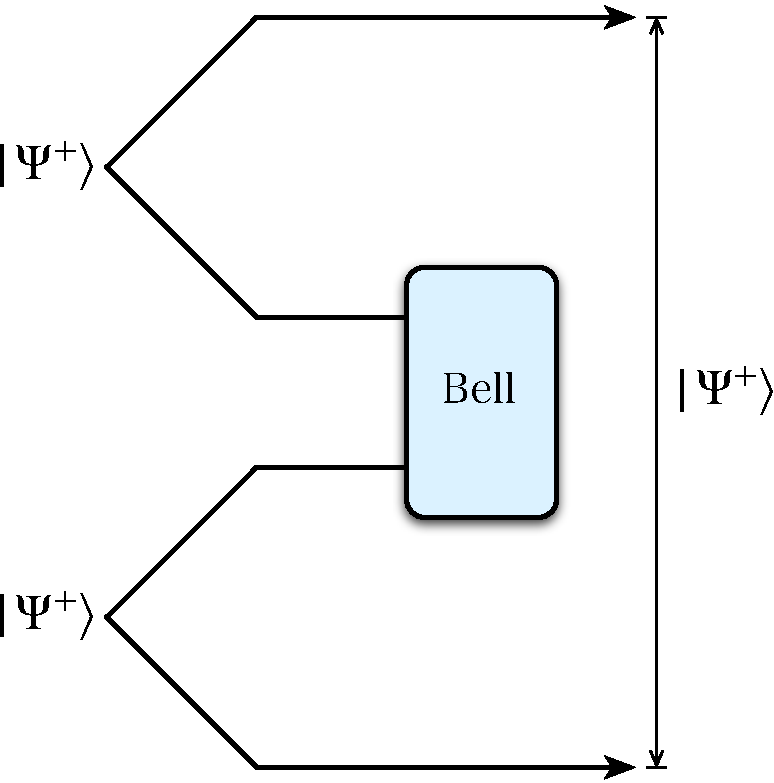
\includegraphics[width=0.7\columnwidth]{figures/Entanglement_swapping}
	\caption{Entanglement swapping takes two Bell pairs in series and performs a Bell measurement between one qubit from each pair. The resultant state is a longer-range Bell pair between the remaining two qubits.} \label{fig:swapping}
\end{figure}

Entanglement purification (see Fig.~\ref{fig:purification}) takes two noisy Bell pairs and transforms them into one less noisy Bell pair \cite{bib:Bennett96}. Specifically, for two Bell pairs of fidelity $F$, a standard purification circuit \cite{pan???} yields a single Bell pair with fidelity,
\begin{align}
F_\mathrm{out} = \frac{{F_\mathrm{in}}^2}{{F_\mathrm{in}}^2 + (1 - {F_\mathrm{in}})^2},
\end{align}
which has the property that so long as \mbox{$F_\mathrm{in}>1/2$}, the output fidelity is higher than the input fidelity, \mbox{$F_\mathrm{out}>F_\mathrm{in}$}, as per Fig.~\ref{fig:purification}(bottom).

\begin{figure}[!htb]
	\centering
	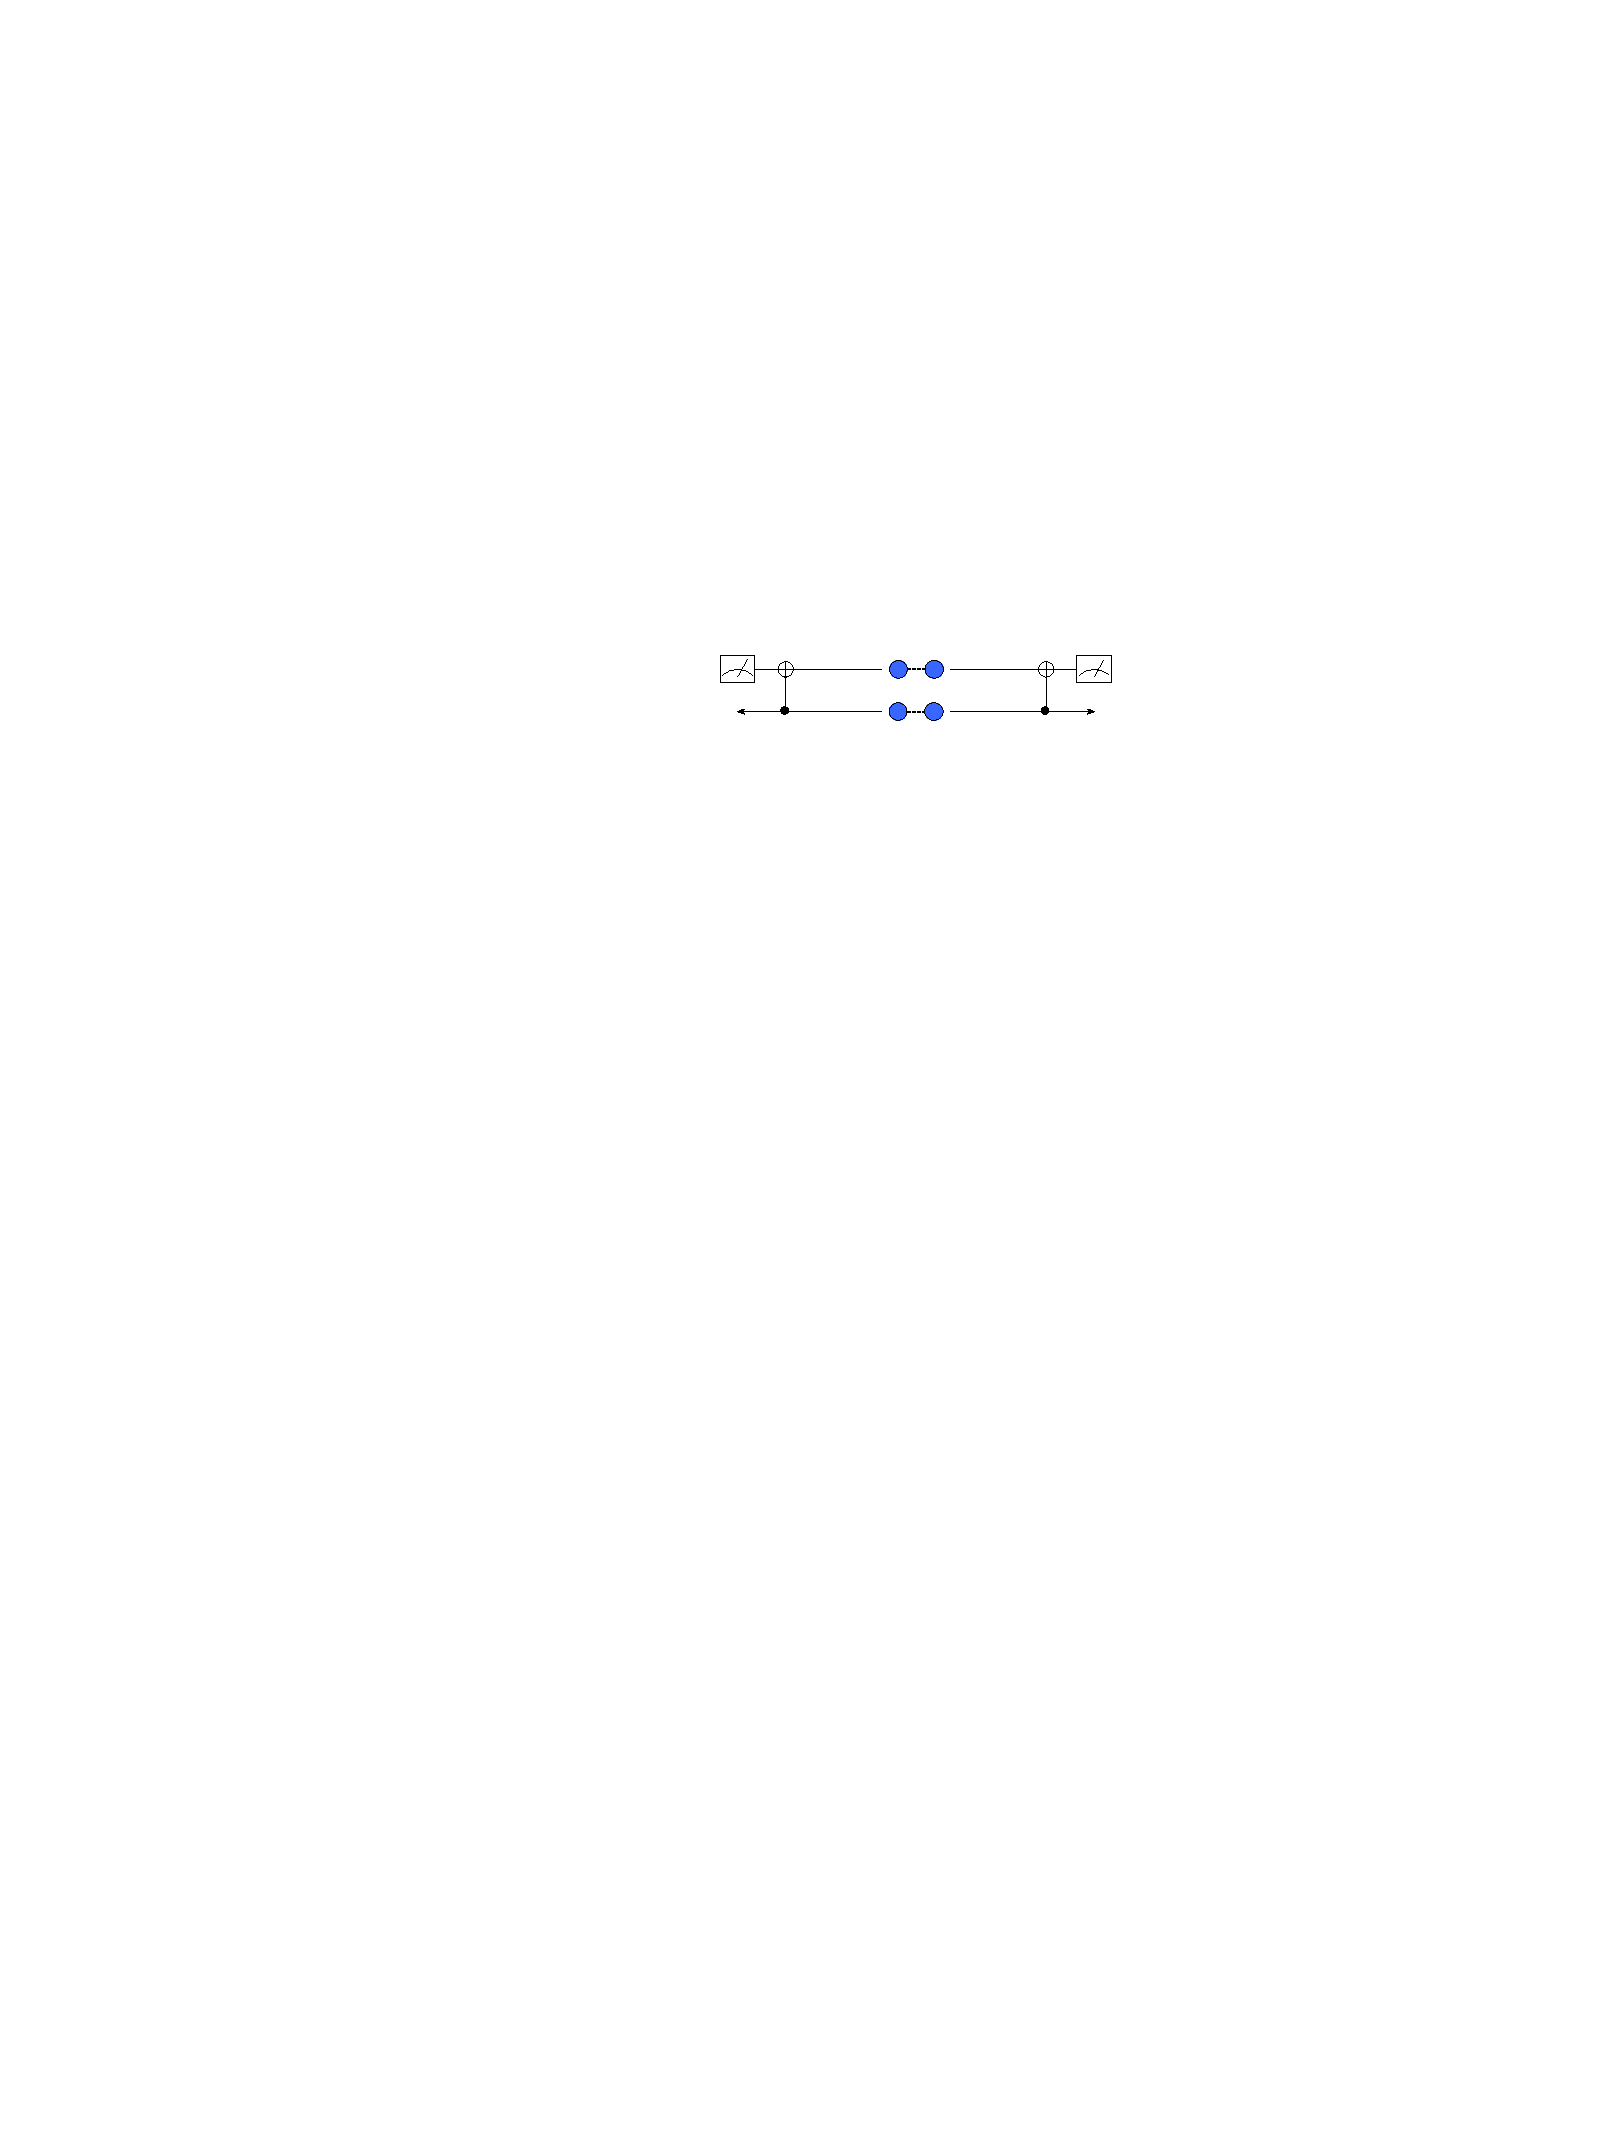
\includegraphics[width=\columnwidth]{figures/Entanglement_purification.pdf}\\
	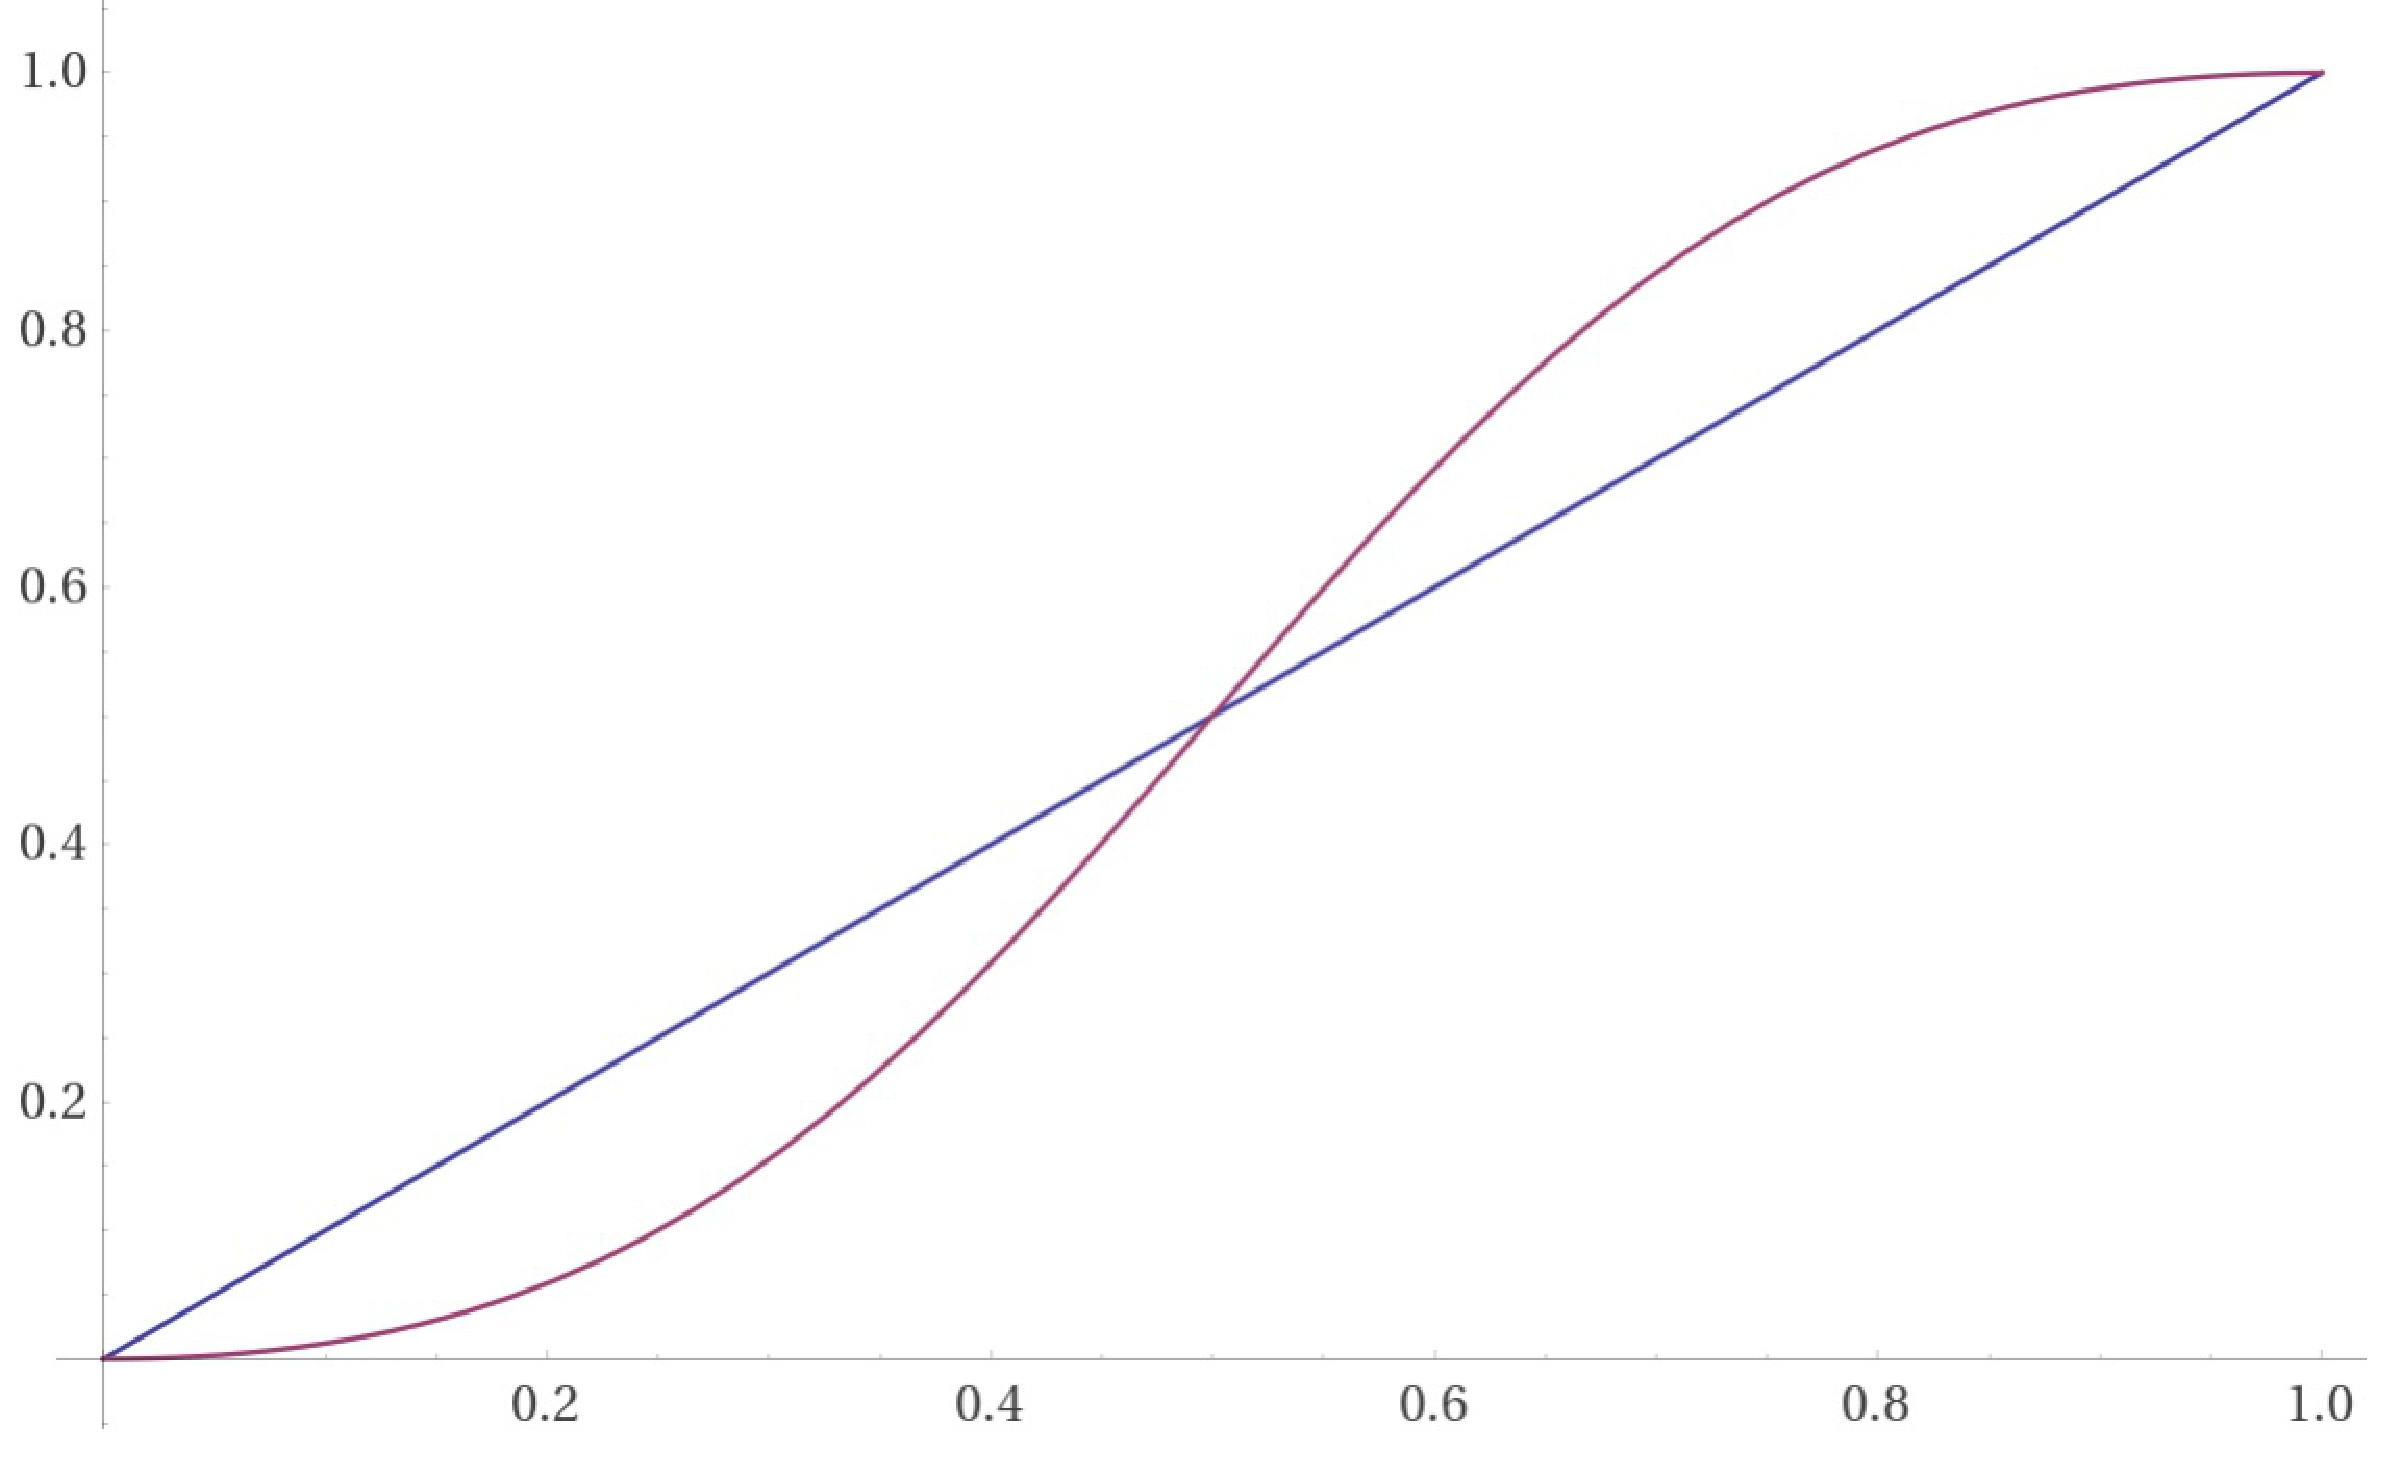
\includegraphics[width=\columnwidth]{figures/Purification_fidelity.pdf}
	\caption{(top) Entanglement purification takes two Bell pairs (shown in blue) and performs partial Bell measurements between corresponding qubits from each pair. The resultant state is a single Bell pair with higher fidelity than either of the originals. (bottom) Input/output relation for the fidelity of Bell pairs undergoing entanglement purification. The straight line acts as a visual guide for equality.} \label{fig:purification}
\end{figure}

Quantum repeaters subdivide our long-range link into shorter segments, interspersed with nodes that perform entanglement swapping to extend range and purification to improve quality (see Fig.~\ref{fig:repeater}).

\begin{figure*}[!htb]
	\centering
	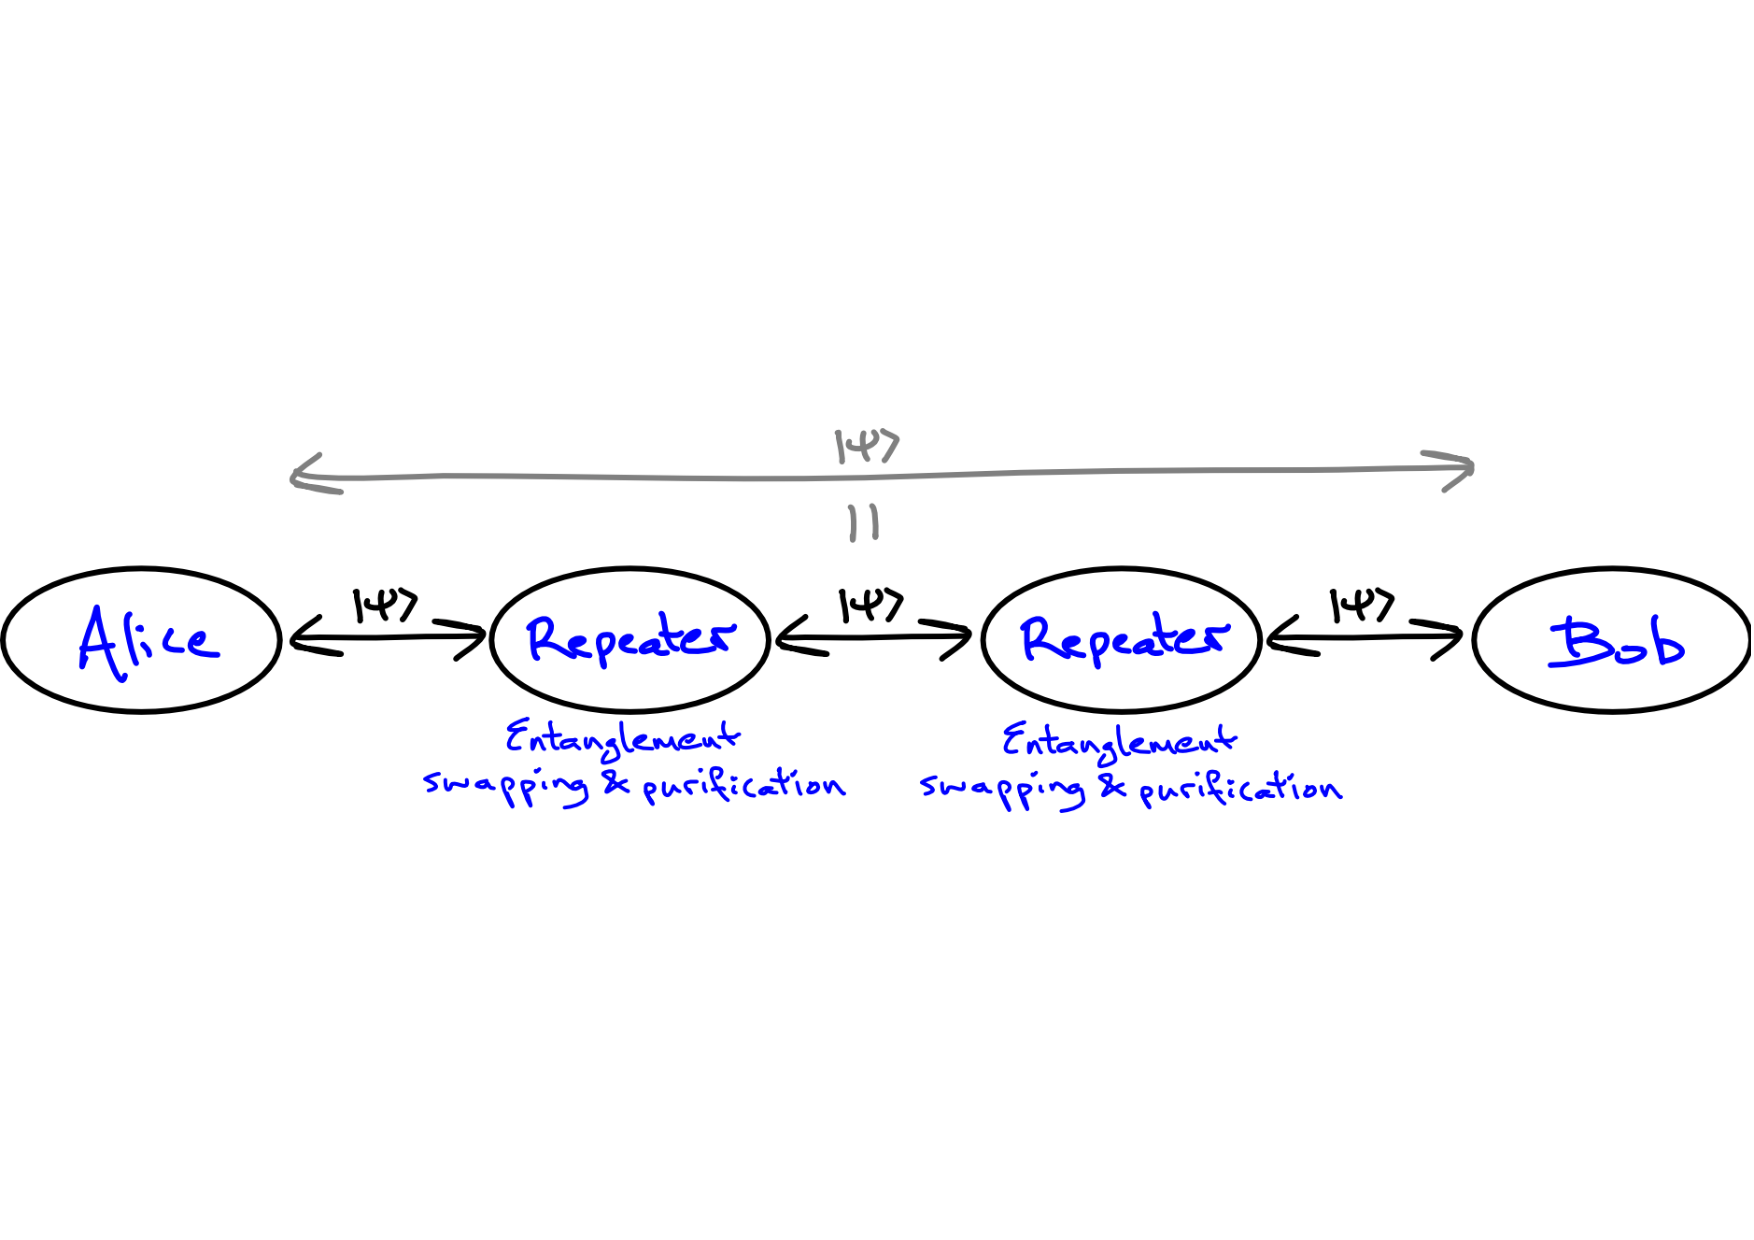
\includegraphics[width=2\columnwidth]{figures/Repeater}
	\caption{A quantum repeater network comprising entanglement links, entanglement swapping, and entanglement purification. Entanglement swapping extends the range of entanglement by `fusing' Bell pairs together, while entanglement purification takes multiple copies of noisy Bell pairs and reduced them down to one of higher quality. Quantum repeaters have the favourable property that efficiency only drops polynomially with distance, as opposed to the exponential decay expected from direct transmission.} \label{fig:repeater}
\end{figure*}

One might immediately question how this overcomes exponential loss. If all the individual segments need to work in the presence of loss, how is the effective loss rate any different to that of the entire length functioning at once? The key is that the individual segments don't need to succeed simultaneously. We employ a divide-and-conquer strategy, whereby we perform entanglement swapping pairwise, rather than all at once, creating slightly longer links. If they fail, we reattempt them. If they succeed, we go up a level and attempt joining the extended links. This necessarily requires high-efficiency, push-button quantum memories, something which is extremely challenging using present-day technology.

We can visualise an entanglement swapping network as a tree graph, where leaf nodes represent Bell pairs, and non-leaf nodes represent entanglement swapping operations. If we were to attempt to perform entanglement swapping in a linear fashion using a naive repeat-until-success strategy, repeatedly fusing on one extra link at a time, we could represent the tree diagram as per Fig.~\ref{fig:rep_linear}, where time flows from bottom to top.

\begin{figure}[!htb]
	\centering
	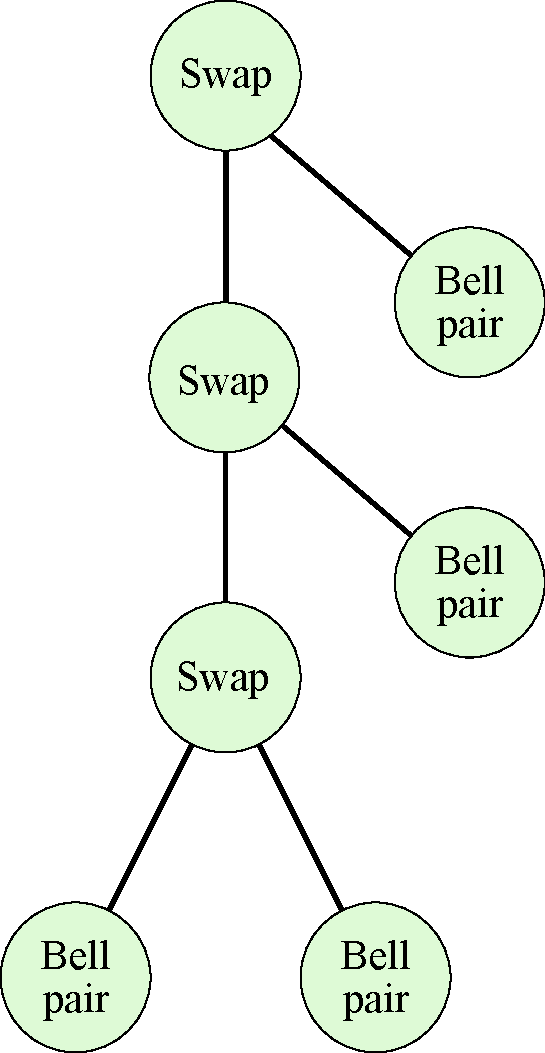
\includegraphics[width=0.5\columnwidth]{figures/Repeater_linear}
	\caption{Entanglement swapping hierarchy for a naïve in-series construction for a quantum repeater network. Time flows from bottom to top. With all swapping operations proceeding in series. This configuration is inefficient and not scalable.} \label{fig:rep_linear}
\end{figure}

Here the depth of the tree represents how many entanglement swapping operations must succeed in series for an overall success, which is linear in the number of Bell pairs and nodes. Any failures as a result of loss or non-deterministic operations whilst progressing up the tree requires us to recommence from the bottom of the tree since failure destroys the state. So the overall success rate drops exponentially with the number of nodes and we see that subdividing the length of the channel into segments achieves nothing in terms of efficiency.

The divide-and-conquer strategy behaves very different on the other hand. We can visualise this as a binary tree graph, as per Fig.~\ref{fig:rep_tree}.

\begin{figure}[!htb]
	\centering
	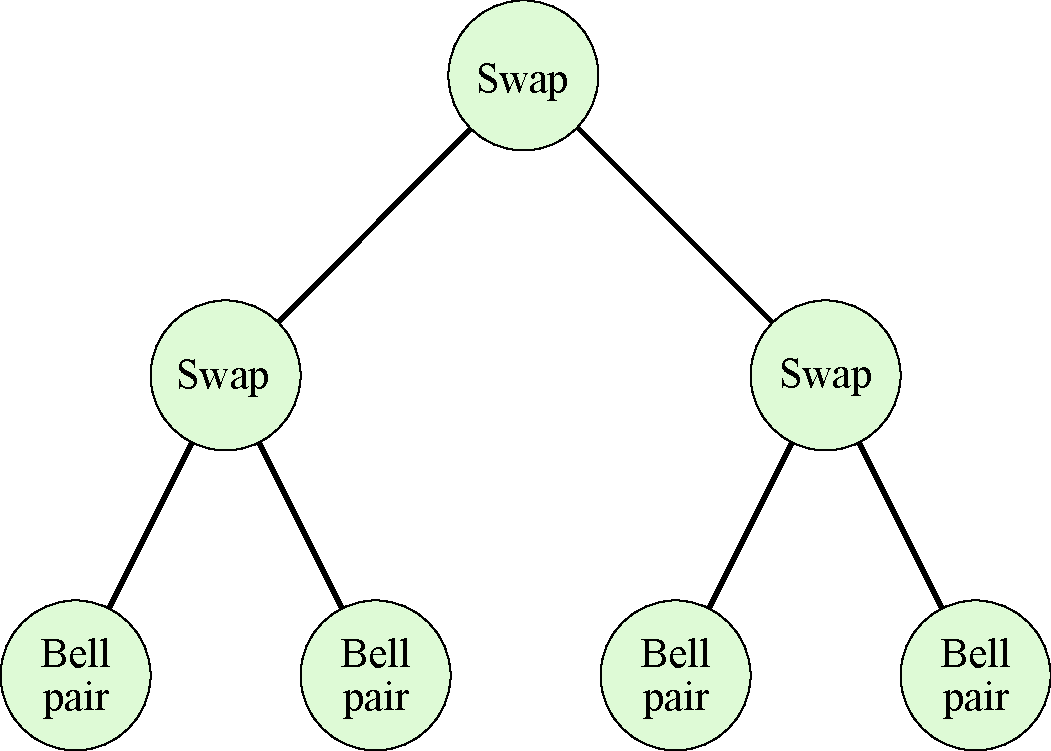
\includegraphics[width=\columnwidth]{figures/Repeater_tree}
	\caption{Entanglement swapping hierarchy for a divide-and-conquer based quantum repeater network. Time flows from bottom to top. Operations proceeding vertically up the graph take place in series, whereas different branches may be performed in parallel. If an operation fails, everything underneath it in the tree must be reattempted. This configuration allows efficient scaling in long-range networks.} \label{fig:rep_tree}
\end{figure}

Going sideways across the tree, things can be performed in parallel. Going upward through the tree they have to succeed in series, as before. When a SWAP operation fails, everything beneath it needs to be repeated, but separate branches are unaffected and can be held in quantum memory should a neighbouring branch need to be reattempted. Note that a binary tree has only logarithmic depth in the number of leaf nodes. The success probability drops exponentially with the depth of the tree, which is logarithmic, resulting in an overall polynomial scaling.

Let $N_i$ be the number of Bell pairs consumed to generate a Bell pair at level $i$ in the tree. Since a swapping operation requires two Bell pairs from the level below, we can write the recursive relationship,
\begin{align}
	N_{n+1} = \frac{2N_n}{p},
\end{align}
where $p$ is the success probability, incorporating loss and device non-determinism. This recursive relationship has the solution,
\begin{align}
	N_n &= L^{\log_2(2/p)} = \mathrm{poly}(L),
\end{align}where there are $L=2^n$ Bell pair segments at the lowest level of the $n$-level hierarchy. The effective efficiency is the inverse of this,
\begin{align}
	\eta = \frac{1}{N_n} = \mathrm{poly}^{-1}(L).
\end{align}

We now have an overhead in creating long-range entanglement with net efficiency scaling only inverse polynomially with distance. In principle, this makes the scheme `efficient' (in the computer science sense) over arbitrary distances. However, the engineering requirements for quantum repeaters are immense, requiring:
\begin{itemize}
	\item Entanglement swapping: to extend range.
	\item Entanglement purification: to improve quality.
	\item Quantum memories: to hold qubits while waiting upon others for further swapping or purification.
\end{itemize}

Each of these ingredients has strict mode-matching requirements to ensure photon indistinguishability, they must all be optimised to the same optical frequency, and must all be highly efficient. The last point is especially relevant to optical quantum memories, which typically suffer significant loss rates associated with input/output coupling and in-memory decay \cite{???}. Additionally, quantum memories must be `push button memories', whereby out-coupling is not random, but classically triggered.

While these individual ingredients have all been demonstrated in isolation, combining them into a long-range repeater network is beyond our current engineering capabilities.

\subsubsection{Trusted nodes} \label{trusted-nodes}

In a trusted node network (see Fig.~\ref{fig:trusted_node}) we again subdivide our long-range link into short segments over which loss rates and bandwidth are tolerable \cite{bib:salvail2010security}. Between each link is a \emph{trusted node}, whose job it is to be the recipient of the QKD key, retransmit it to the next trusted node, and destroy their copy of the key, thereby acting as a relay.

\begin{figure*}[!htb]
	\centering
	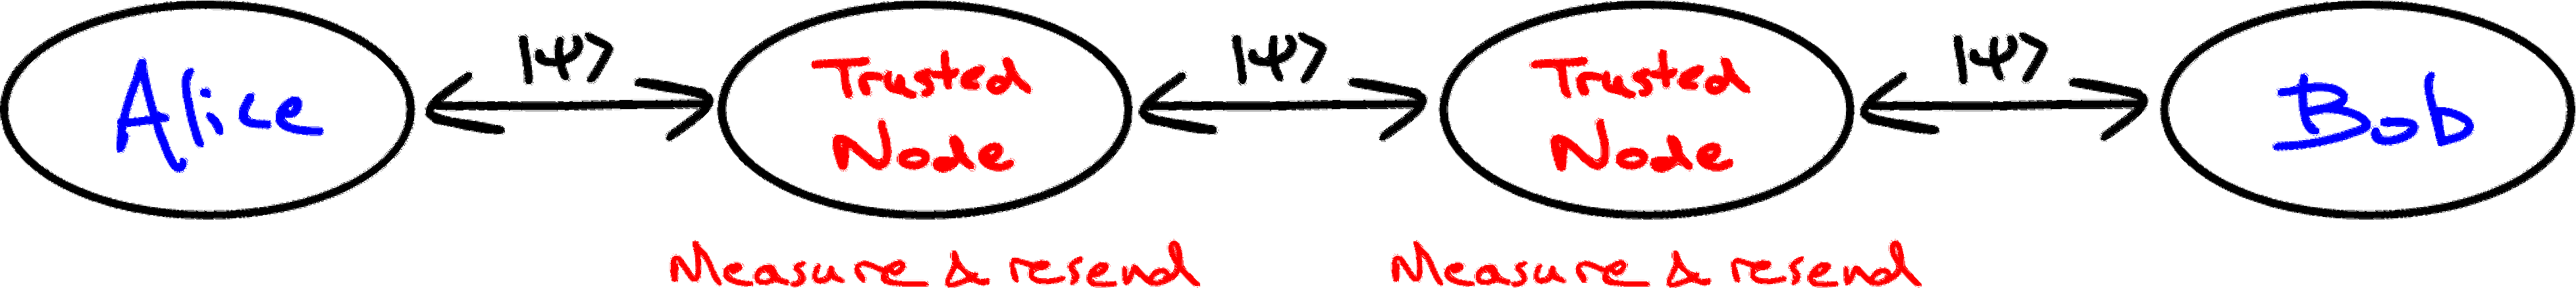
\includegraphics[width=2\columnwidth]{figures/Trusted_node}
	\caption{A trusted node network between Alice and Bob. The intermediate	nodes are necessary to overcome exponential loss against distance, but must be trusted to not compromise the key bits they measure and resend.} \label{fig:trusted_node}
\end{figure*}

Mathematically, the success rate of a link of length $L$ scales inverse exponentially as,
\begin{align}
	P(L) = e^{-\beta L},
\end{align}
where $\beta>0$ characterises loss per distance. If we subdivide the link length $L$ into $n$ segments, each segment will have length,
\begin{align}
	L_\mathrm{seg} = \frac{L}{n},
\end{align}
	with success rate,
\begin{align}
	P(L_\mathrm{seg}) = e^{-\beta L/n}.
\end{align}
With $n$ such links required to succeed in succession (not simultaneously), the overall success rate is,
\begin{align}
	P_\mathrm{net}(n) = \frac{P(L_\mathrm{seg})}{n} = \frac{P(L/n)}{n} = \frac{e^{-\beta L/n}}{n},
\end{align}
resulting in a trade-off from the exponential term into a linear term. In the large $n$ limit this scaling reduces to,
\begin{align}
	\lim_{n\to\infty} P_\mathrm{net}(n) = \frac{1}{n},
\end{align}
implying a linear number of repetitions are required to achieve success.

Although this type of intercept-resend strategy requires only linear time overhead in distance, its utility is limited to QKD as it does not distribute entanglement, only secret key bits. It suffers the obvious flaw that because it is based on intercept-resend --- also a type of attack --- the nodes must be absolutely secure, hence the name `trusted nodes'. If just a single node is compromised, so is the entire channel. The likelihood of the route being secure therefore drops exponentially with the number of trusted nodes --- we've effectively traded exponential photon loss for exponential security loss. Despite this limitation, for highly specialised purposes, such as point-to-point communication where all nodes are controlled by the same party, this provides security as good as the armed guards protecting them. This is the approach used in present-day long-range QKD links, most notably in China's extremely impressive national QKD network (see Fig.~\ref{fig:china_network}).

\begin{figure*}[!htb]
	\centering
	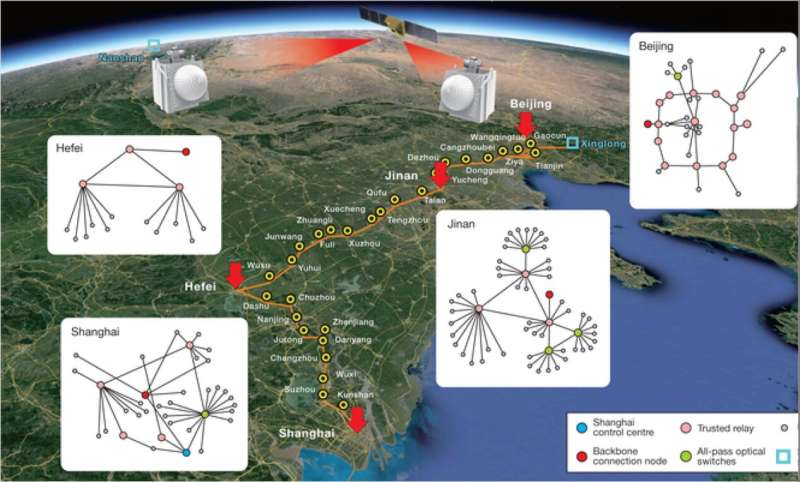
\includegraphics[width=2\columnwidth]{figures/China_network.jpeg}
	\caption{China's national quantum key distribution network, comprising a number of city-wide networks, a major backbone, and a long-range satellite. The network is based on trusted nodes as opposed to quantum repeaters. (Ask permission???)}	\label{fig:china_network} %???
\end{figure*}

\subsubsection{Multi-path QKD with trusted nodes}\label{multi-path-qkd-with-trusted-nodes}

Since a trusted node network requires that all nodes be secure, security drops exponentially with the number of trusted nodes --- if just one is compromised so is the key. This is a highly undesirable scaling characteristic, yet simultaneously appears the price to pay for relying on trusted nodes rather than quantum repeaters. This can however be improved upon without turning to quantum repeaters. The key, paradoxically, is to use \emph{more} nodes, but in parallel rather than in series.

We achieve this improvement by employing multiple routes through the network, each of which provides its own key. These keys are all combined to yield the master key (see Fig.~\ref{fig:multi_path}),
\begin{align}
	k_\textrm{master} = \bigoplus_i k_i.
\end{align}

The main observation here is that if multiple keys are independently routed, the master key is secure if \emph{any} of the constituent keys was secure. Equivalently, the key is only compromised if \emph{all} path keys $k_i$ are known. This achieves exponential scaling in the opposite direction --- security increases exponentially with the number of keys independently routed in parallel. We now have two exponentials: security decreases exponentially with the number of nodes in series and increases exponentially with the number of keys in parallel.

\begin{figure}[!htb]
	\centering
	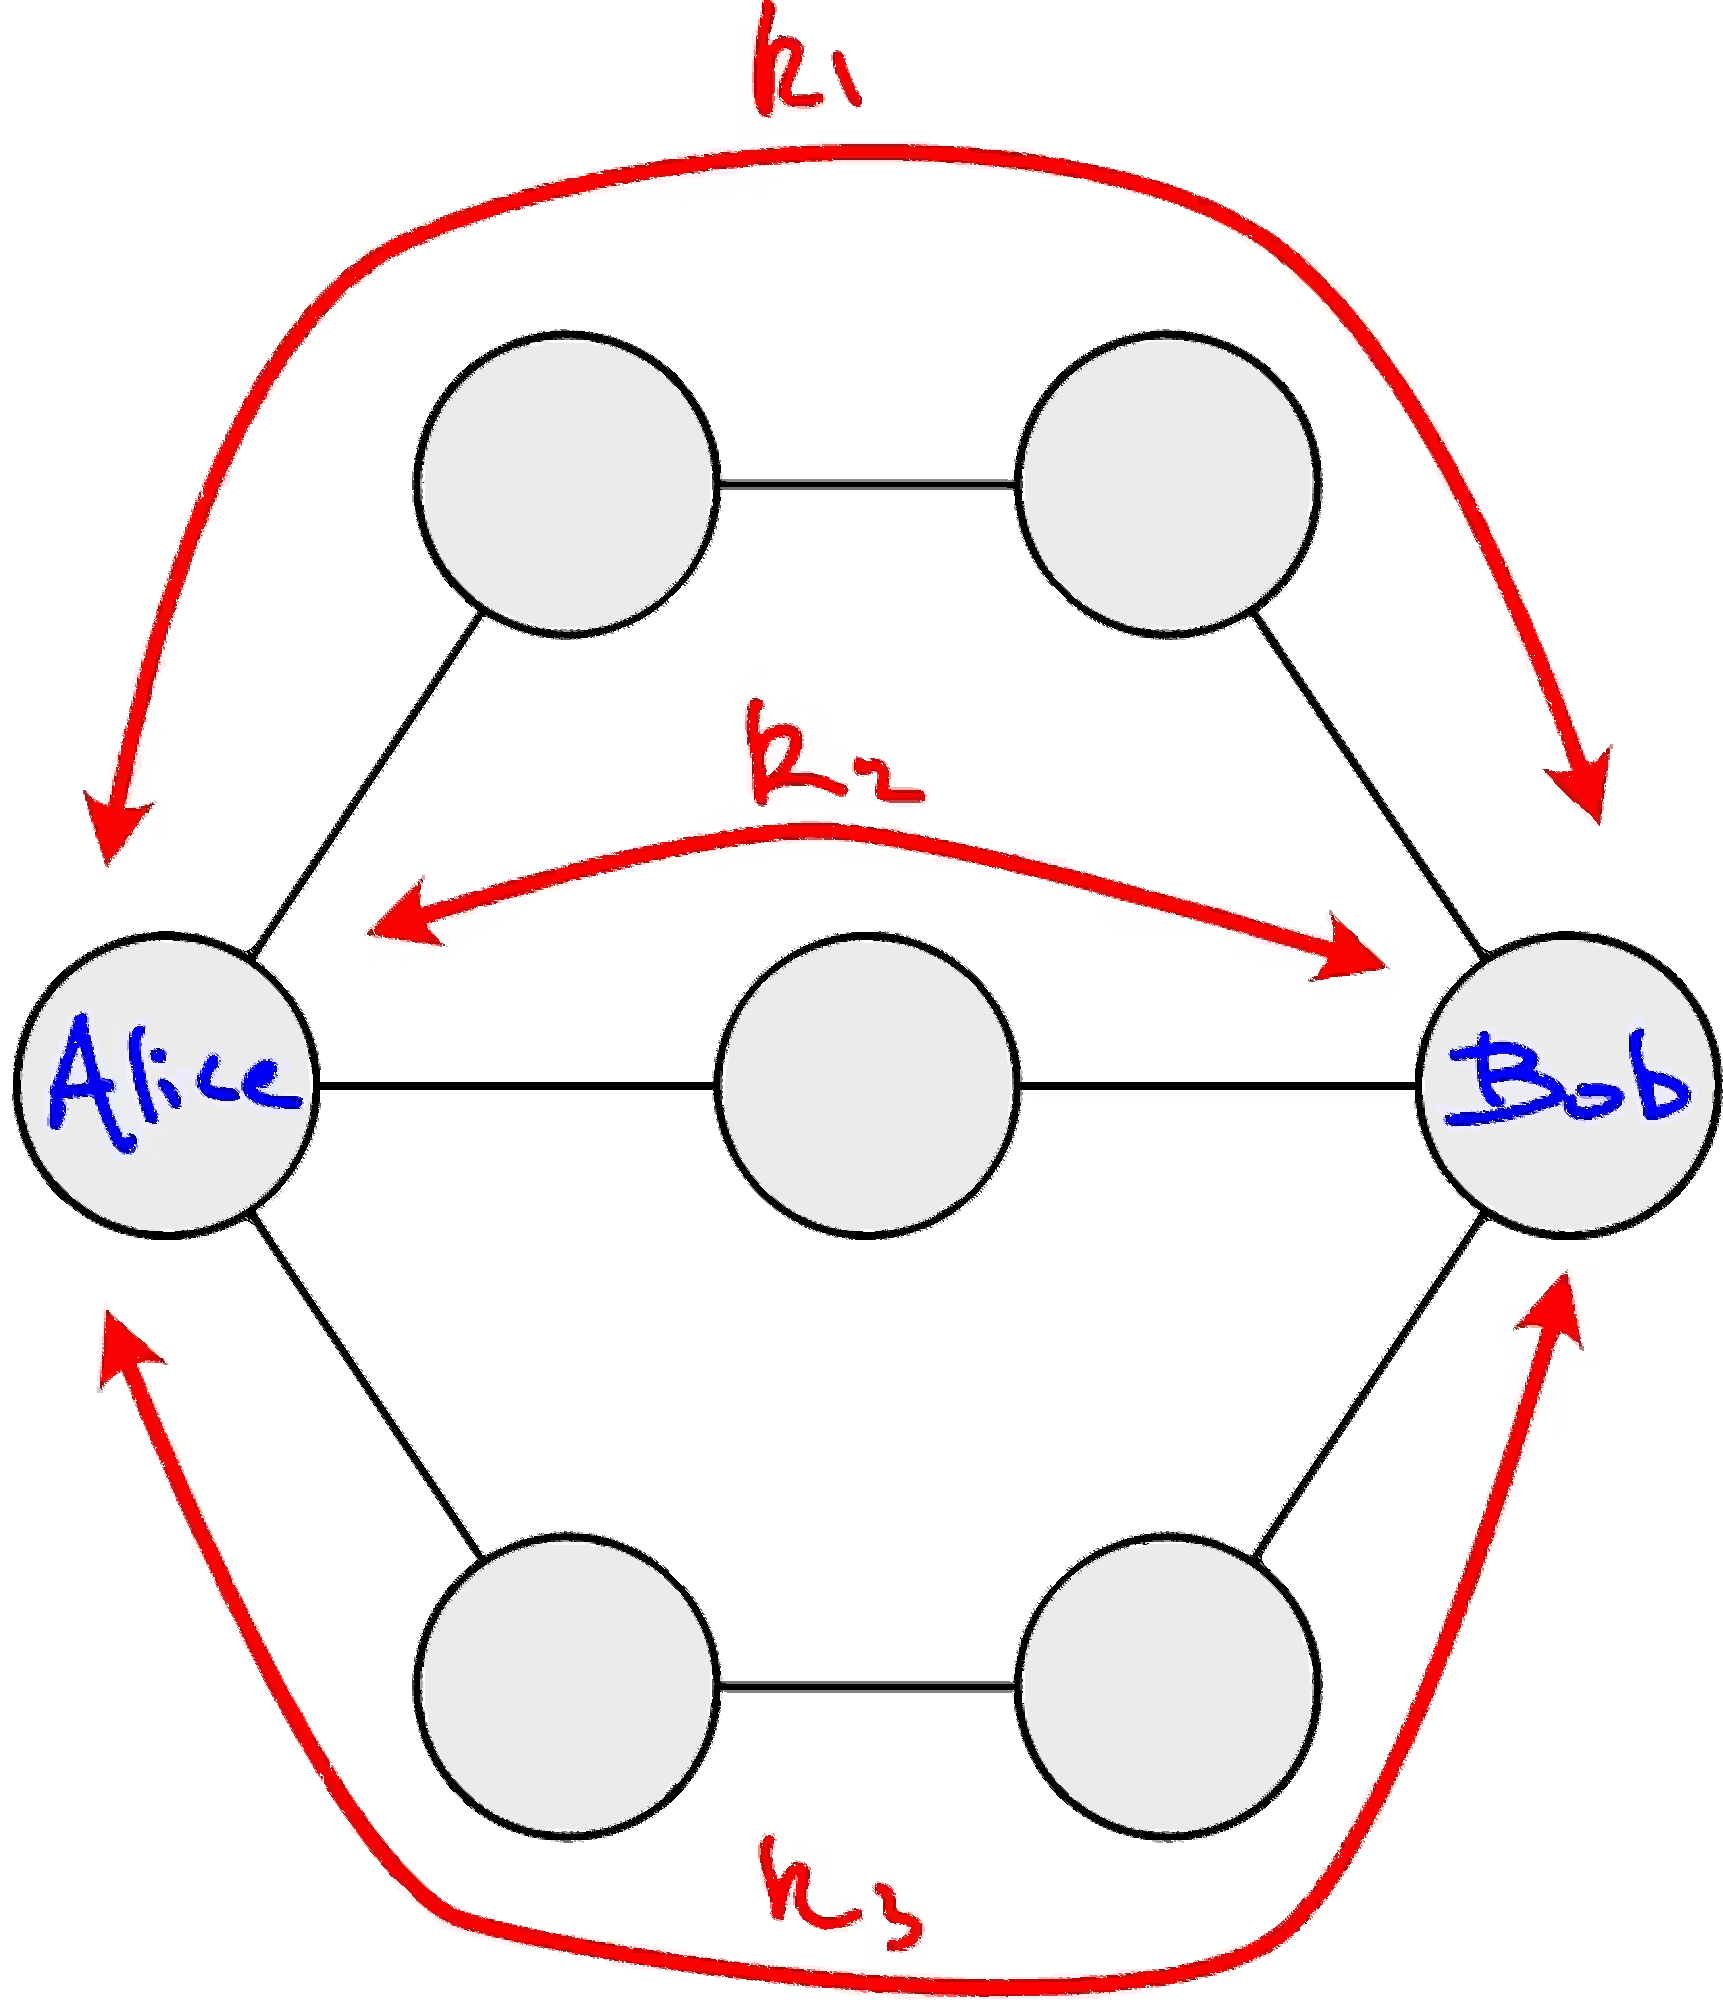
\includegraphics[width=0.6\columnwidth]{figures/Trusted_node_multipath}
	\caption{A multi-path trusted node QKD network. So long as there exists at least one path between Alice and Bob which is not compromised, a secure key may be established.} \label{fig:multi_path}
\end{figure}

We can easily derive a statistical model for the security of this network. Let $P(w_i)$ be the probability of node $i$ in path $w$ not being compromised. For a given path of length $L$, the path is secure if \emph{all} nodes are secure. Hence,
\begin{align}
	P_{\rm path}(w) = \prod_{i=1}^L P_{\rm node}(w_i).
\end{align}
For multiple paths, the key is secure if \emph{any} path is secure since all individual path keys $k_i$ must be compromised for $k_\mathrm{master}$ to be compromised. Thus for a set of $N$ vertex-independent paths through a network,
\begin{align}
	P_{\rm net}(\vec{w}) = 1-\prod_{i=1}^N [1-P_{\rm path}(w_i)].
\end{align}
If we make the simplifying assumption that all nodes have the same security $P_{\rm node}$ then a statistically independent model yields,
\begin{align}
	P_{\rm path}(L) &= {P_{\rm node}}^{L-2},\nonumber\\
	P_{\rm net}(N) &= 1-\prod_{i=1}^N (1-{P_{\rm node}}^{L_i-2}).
\end{align}
Making a further simplifying assumption that there are $N$ parallel paths all of length $L$, we obtain,
\begin{align}
	P_{\rm net} = 1-(1-{P_{\rm node}}^{L-2})^N.
\end{align}
Thus we see that individual paths have security that drops exponentially in their length, while the security of all paths jointly increases exponentially with the number of constituent paths. Importantly, for any value of $P_{\rm node}$, an appropriate choice of $N$ allows $P_{\rm net}$ to become arbitrarily close to 1.

\subsubsection{Channel authentication} \label{channel-authentication}

Although QKD in principle offers perfect security between two users, the robustness against man-in-the-middle attacks is based upon the assumption that those users know they are speaking to one another rather than an intermediary. This requires authentication via a classical channel. Ordinarily, we do this classically using digital signatures. However, our most popular current approaches for doing this (RSA \& ECC) are vulnerable to quantum attacks. To overcome this we can use one of two approaches:
\begin{itemize}
	\item Authentication using shared secrets, as discussed in Sec.~\ref{authentication-using-shared-secrets}.
	\item Authentication using post-quantum digital signatures, to be discussed in Sec.~\ref{post-quantum-cryptography-pqc}.
\end{itemize}
Both of these approaches are based on the security of hash functions, which we strongly believe to be robust against quantum attack vectors. In either case, some amount of data must be securely shared via other means, making QKD only as secure as whatever this alternate channel is. However, this shared secret is something that only needs to be shared once, and can be reused, unlike the one-time-pad key.

\subsection{Quantum anonymous broadcasting}

Quantum key distribution is a simple yet secure two-party cryptographic protocol. However, by employing multi-partite entanglement more elaborate cryptographic protocols can be constructed. One such protocol is \emph{quantum anonymous broadcasting} \cite{bib:QAB}, whereby users in a group are able to broadcast messages for all to hear, but such that the speaker's identity remains concealed.

To achieve this we rely on the distribution of multi-party GHZ states of the form
\begin{align}
	\ket\psi_\mathrm{GHZ}^{(N)} = \frac{1}{\sqrt{2}}(\ket{0}^{\otimes N} + \ket{1}^{\otimes N}),
\end{align}
where there are $N$ parties, each of whom receive one qubit from the collectively entangled state. GHZ states have the property that the action of a Pauli-$\hat{Z}$ gate on the state is independent of which qubit it is applied to,
\begin{align}
	\hat{Z}_i \ket\psi_\mathrm{GHZ}^{(N)} = \frac{1}{\sqrt{2}}(\ket{0}^{\otimes N} - \ket{1}^{\otimes N})\,\,\forall\, i.
\end{align}

If we let $m_i=\{0,1\}$ be the message of the $i$th user, then that user broadcasts their message by applying $\hat{Z}_i^{m_i}$ to their qubit, as per Fig.~\ref{fig:QAB}. If we impose the constraint that only one user speaks at a time, this has the effect of encoding $m_i$ into the phase of the GHZ state. Note that individual users always observe their reduced state to be the maximally mixed state, independent of $\vec m$,
\begin{align}
	\mathrm{tr}_{\bar i}(\hat{Z}_{j}^{m_j} \ket\psi_\mathrm{GHZ}^{(N)}\bra\psi_\mathrm{GHZ}^{(N)}\hat{Z}_{j}^{m_j}) = \frac{\hat{I_i}}{2}\,\,\forall\, i,j,
\end{align}
and are therefore unable to extract any information on their own.

\begin{figure}[!htb]
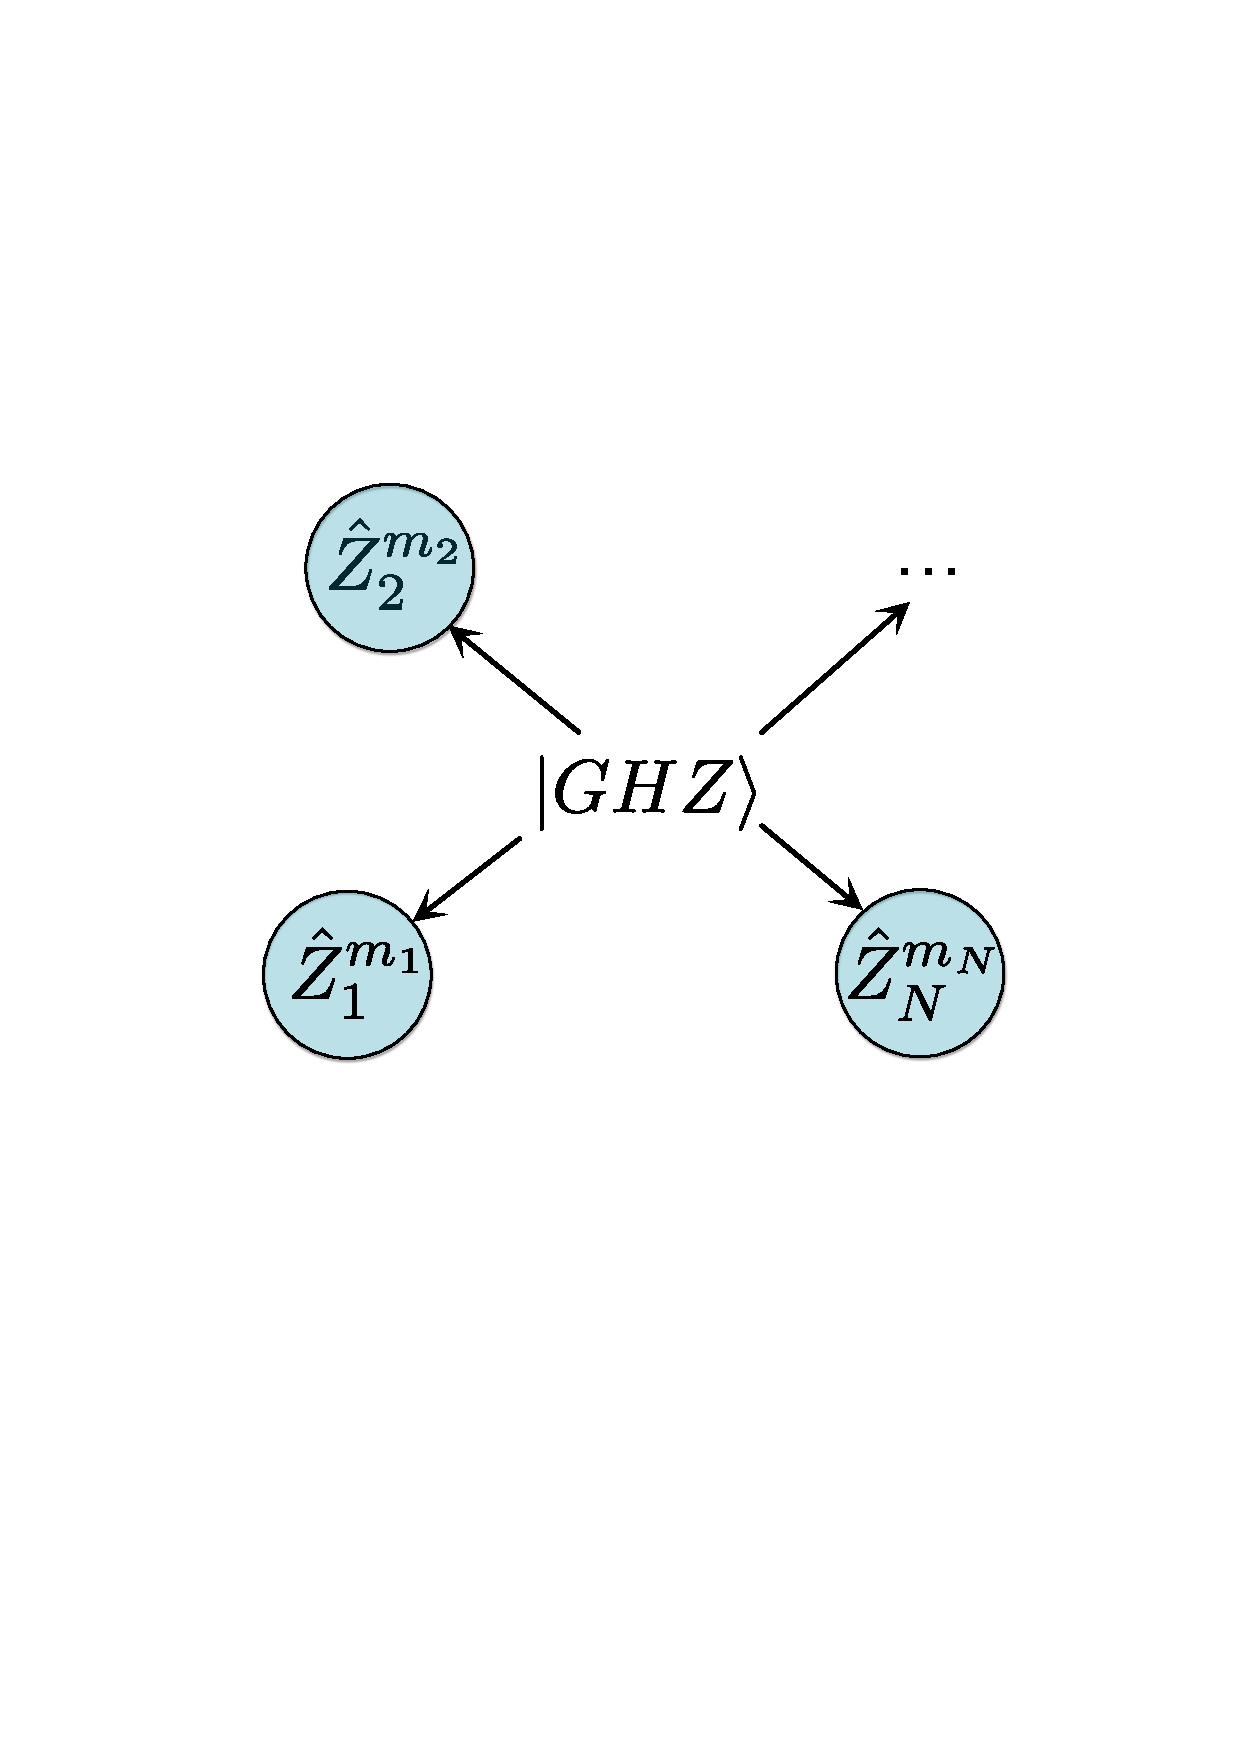
\includegraphics[width=0.6\columnwidth]{figures/QAB}
\caption{Quantum anonymous broadcasting protocol. The network distributes a $N$-qubit GHZ state between the $N$ users. User $i$ broadcasts their message by applying $\hat{Z}_i^{m_i}$ to their qubit. Subsequently, all users measure their qubits in the Pauli-$\hat{X}$ basis and publicly announce their results. The parity of all announced measurement results stipulates \mbox{$m=\bigoplus_{i=1}^N m_i$}. In the case where only one user broadcasts at a time, say user $i$, this reduces to $m_i$.} \label{fig:QAB}
\end{figure}

While the phase relationship in a GHZ state cannot be determined by any user, it can be determined collectively. If following the message broadcast all users measure their qubits in the Pauli-$\hat{X}$ basis (projecting onto \mbox{$\ket\pm = (\ket{0}\pm\ket{1})/\sqrt{2}$}), the parity of these collective measurement results stipulates the phase. Thus, following measurement all users publicly announce the outcome of their $\hat{X}$ measurements from which the phase, and hence message, becomes known to all.

It should be noted that while this simple protocol does offer information theoretic anonymisation of the speaker's identity, it suffers some significant limitations:
\begin{itemize}
\item Strictly only one user may broadcast at a time. If multiple users broadcast simultaneously, the reconstructed message will be given by the XOR of all broadcasters' messages,
	\begin{align}
		m = \bigoplus_{i=1}^{N} m_i.
	\end{align}
	This arises since message encoding is via the Pauli-$\hat{Z}$ operator, which accumulates modulo 2.
\item It is assumed all users are honest when announcing their measurement outcomes. A single dishonest user can disrupt the integrity of broadcast messages by dishonestly announcing random measurement outcomes. Thus, denial-of-service is trivial for anyone in possession of a qubit from the initially distributed GHZ state.
\end{itemize}

\subsection{Quantum anonymous voting}

The idea of using phase encoding to conceal identity can be generalised to \emph{quantum voting} \cite{bib:quantum_voting}, shown in Fig.~\ref{fig:quantum_voting}, where the goal is to implement a multi-party ballot such that users' individual voting decisions remain anonymised but their cumulative value can be collectively determined.

To do so we begin with a different type of entangled state, known as a \emph{ballot state},
\begin{align}
\ket{B} = \frac{1}{\sqrt{N+1}} \sum_{n=0}^N \ket{N-n}_T\otimes\ket{n}_V,
\end{align}
expressed in an occupation number representation, where $\ket{n}$ denotes an $n$-particle state, for example a photon-number state. This is a two-party state, where $V$ denotes the state held at the voting booth while $T$ is held by the tallyman.

Voters cast their votes sequentially, doing so by applying a \emph{voter operator} to the state held at the voting booth. The voter operator for the $i$th voter is defined via a phase-shift operator with angle $\delta_i$,
\begin{align}
\hat{v}_i = e^{i\hat{n}_V\delta_i},	
\end{align}
where $\hat{n}_V = \hat{a}^\dag_V\hat{a}_V$ is the (e.g photon-) number operator for mode $V$, and $\delta_i$ denotes the value of the $i$th voter's vote. 

The collective action of all voters is,
\begin{align}
\hat{v} &= \prod_{i=1}^{N_V} \hat{v}_i = e^{i\hat{n}\Delta}.
\end{align}
where,
\begin{align}
\Delta = \sum_{i=1}^{N_V} \delta_i,
\end{align}
is the cumulative vote.

When applied to the initial ballot state this yields,
\begin{align}
\ket{B'} = \frac{1}{\sqrt{N+1}} \sum_{n=0}^N e^{in\Delta} \ket{N-n}_T\otimes\ket{n}_V,
\end{align}
where the cumulative vote is encoded into the phases of the evolved ballot state.

Similar to quantum anonymous broadcasting, the voting booth and tallyman on their own observe the completely mixed reduced state,
\begin{align}
\mathrm{tr}_{V,T}(\ket{B'}\bra{B'}) &= \frac{1}{N+1} \sum_{n=0}^N \ket{n}_{T,V}\bra{n}_{T,V},
\end{align}
and are therefore unable to extract any information from it.

However, $\Delta$ can be extracted from the collective bipartite state $\ket{B'}$. Thus, the final stage is for the voting booth state to be reunited with the tallyman, who is now able to directly infer $\Delta$ using an appropriate measurement basis on $\ket{B'}$. Specifically, the tallyman measures the expectation value of the \emph{tally operator}, defined as,
\begin{align}
\hat{T} &= \sum_{n=0}^N n\ket{T_n}\bra{T_n},\nonumber\\
\hat{T}_n &= \frac{1}{\sqrt{N+1}} \sum_{k=0}^N e^\frac{2\pi ink}{N+1} \ket{N-k,k},
\end{align}
from which $\Delta$ is obtained via,
\begin{align}
\Delta = \frac{2\pi}{N+1}\bra{B'}\hat{T}\ket{B'}.
\end{align}

\begin{figure}[!htb]
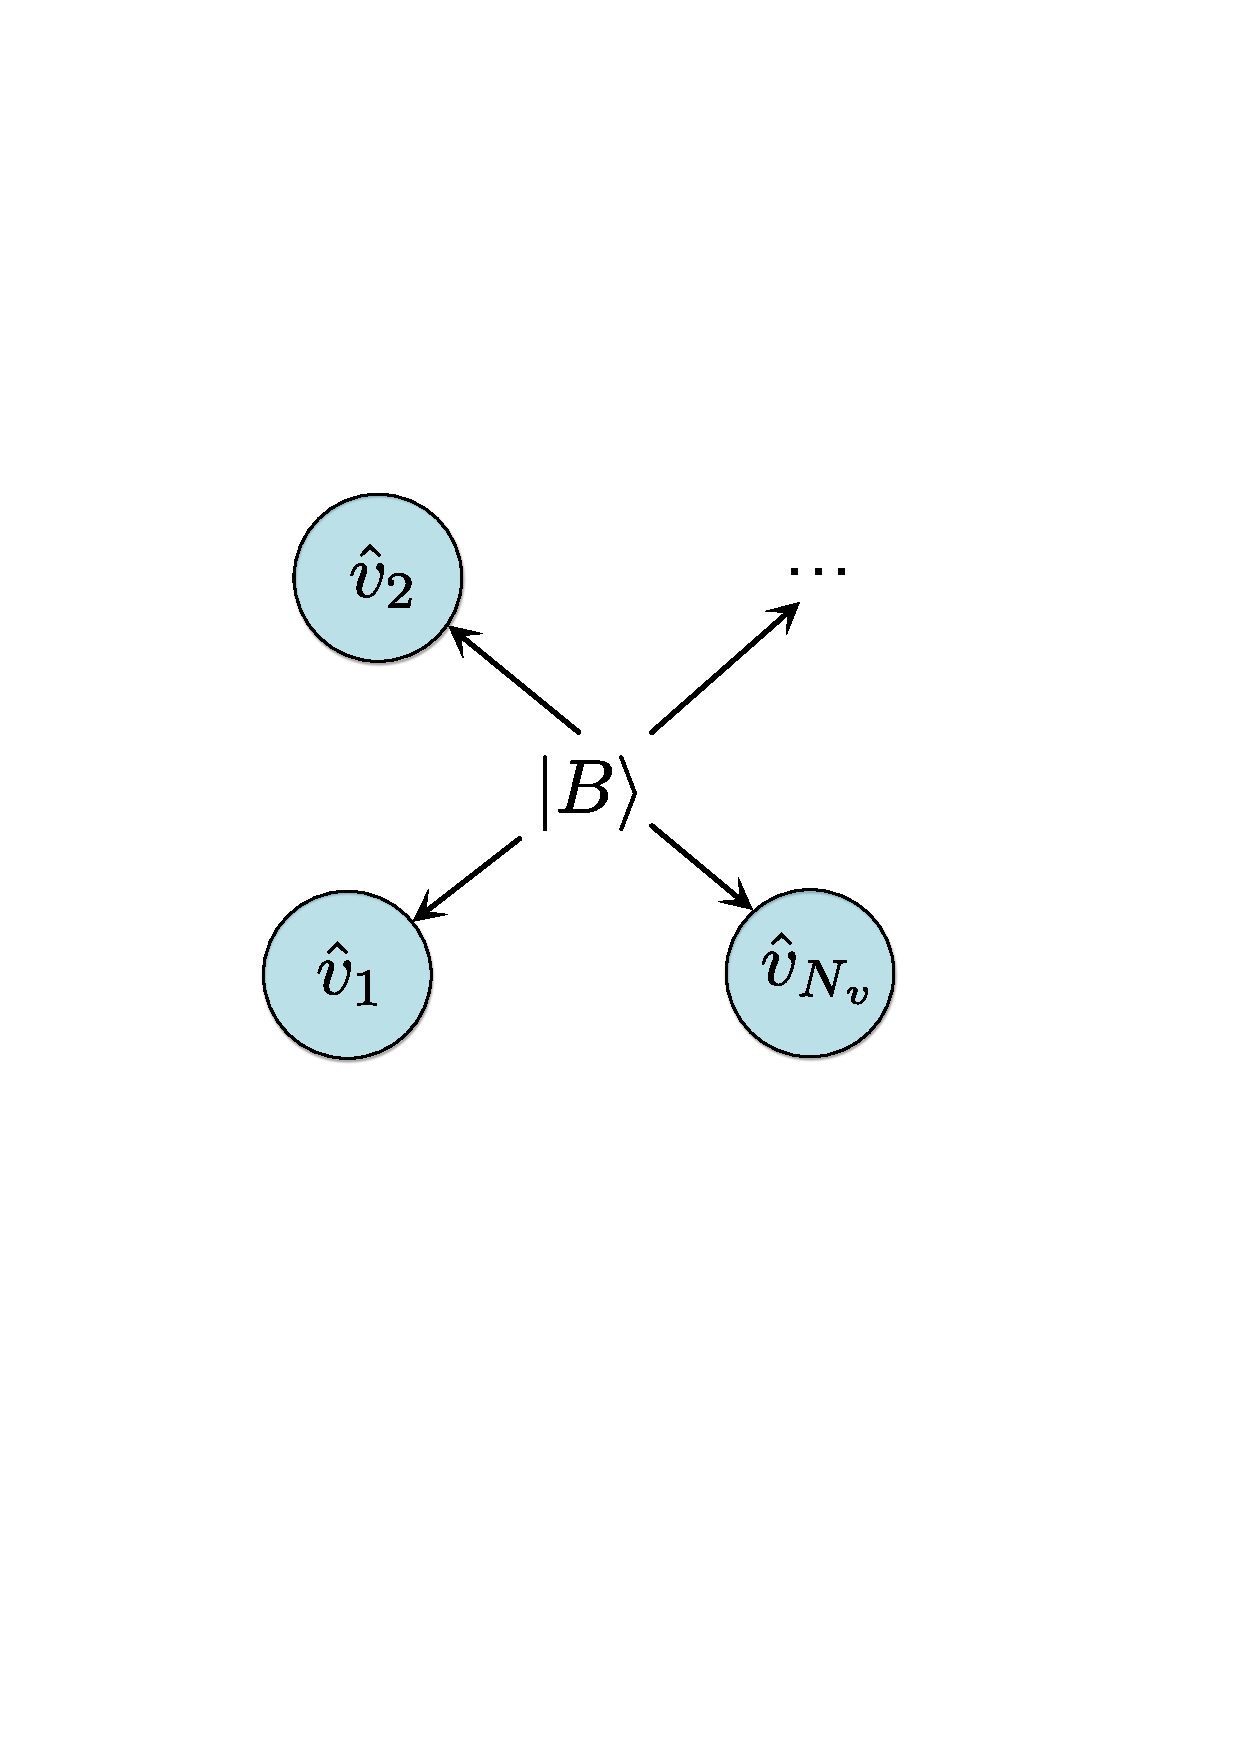
\includegraphics[width=0.6\columnwidth]{figures/quantum_voting}
\caption{Quantum anonymous voting protocol. The network distributes a bipartite \emph{ballot state} between voting booth and tallyman. All voters apply \emph{voter operators}, which encode the value of their vote into the phases in the ballot state. Following voting, the tallyman measures the joint bipartite state in an appropriate basis to recover the phase, which reflects the cumulative vote.} \label{fig:quantum_voting}
\end{figure}

\subsection{Secure quantum computation}

Until now we have focussed primarily on the security of messages. Future quantum computers are likely to be extremely expensive and owned by few. The most common model for utilising them will likely be via outsourcing them to the cloud. The types of computations performed by quantum computers are likely to be very valuable, potentially carrying important IP, trade secrets or information with national security implications. When we outsource things to the cloud today we are only protected by trust --- if the supercomputer we're outsourcing to gets hacked or is dishonest, they'll get all our important data. This raises the issue of encrypting computations as opposed to simply messages --- can a computation be outsourced such that the server executing the computation remains oblivious to the data they are processing?

\subsubsection{Homomorphic encryption} \label{homomorphic-encryption}

\emph{Homomorphic encryption} is a form of encryption whereby data is encrypted by a client and processed on a server \emph{in encrypted form}. That is, the server does not need to decrypt the data to execute computations on it, and returns the output to the client in encrypted form without knowing what it is (see Fig.~\ref{fig:QHE_model}).

\begin{figure}[!htb]
	\centering
	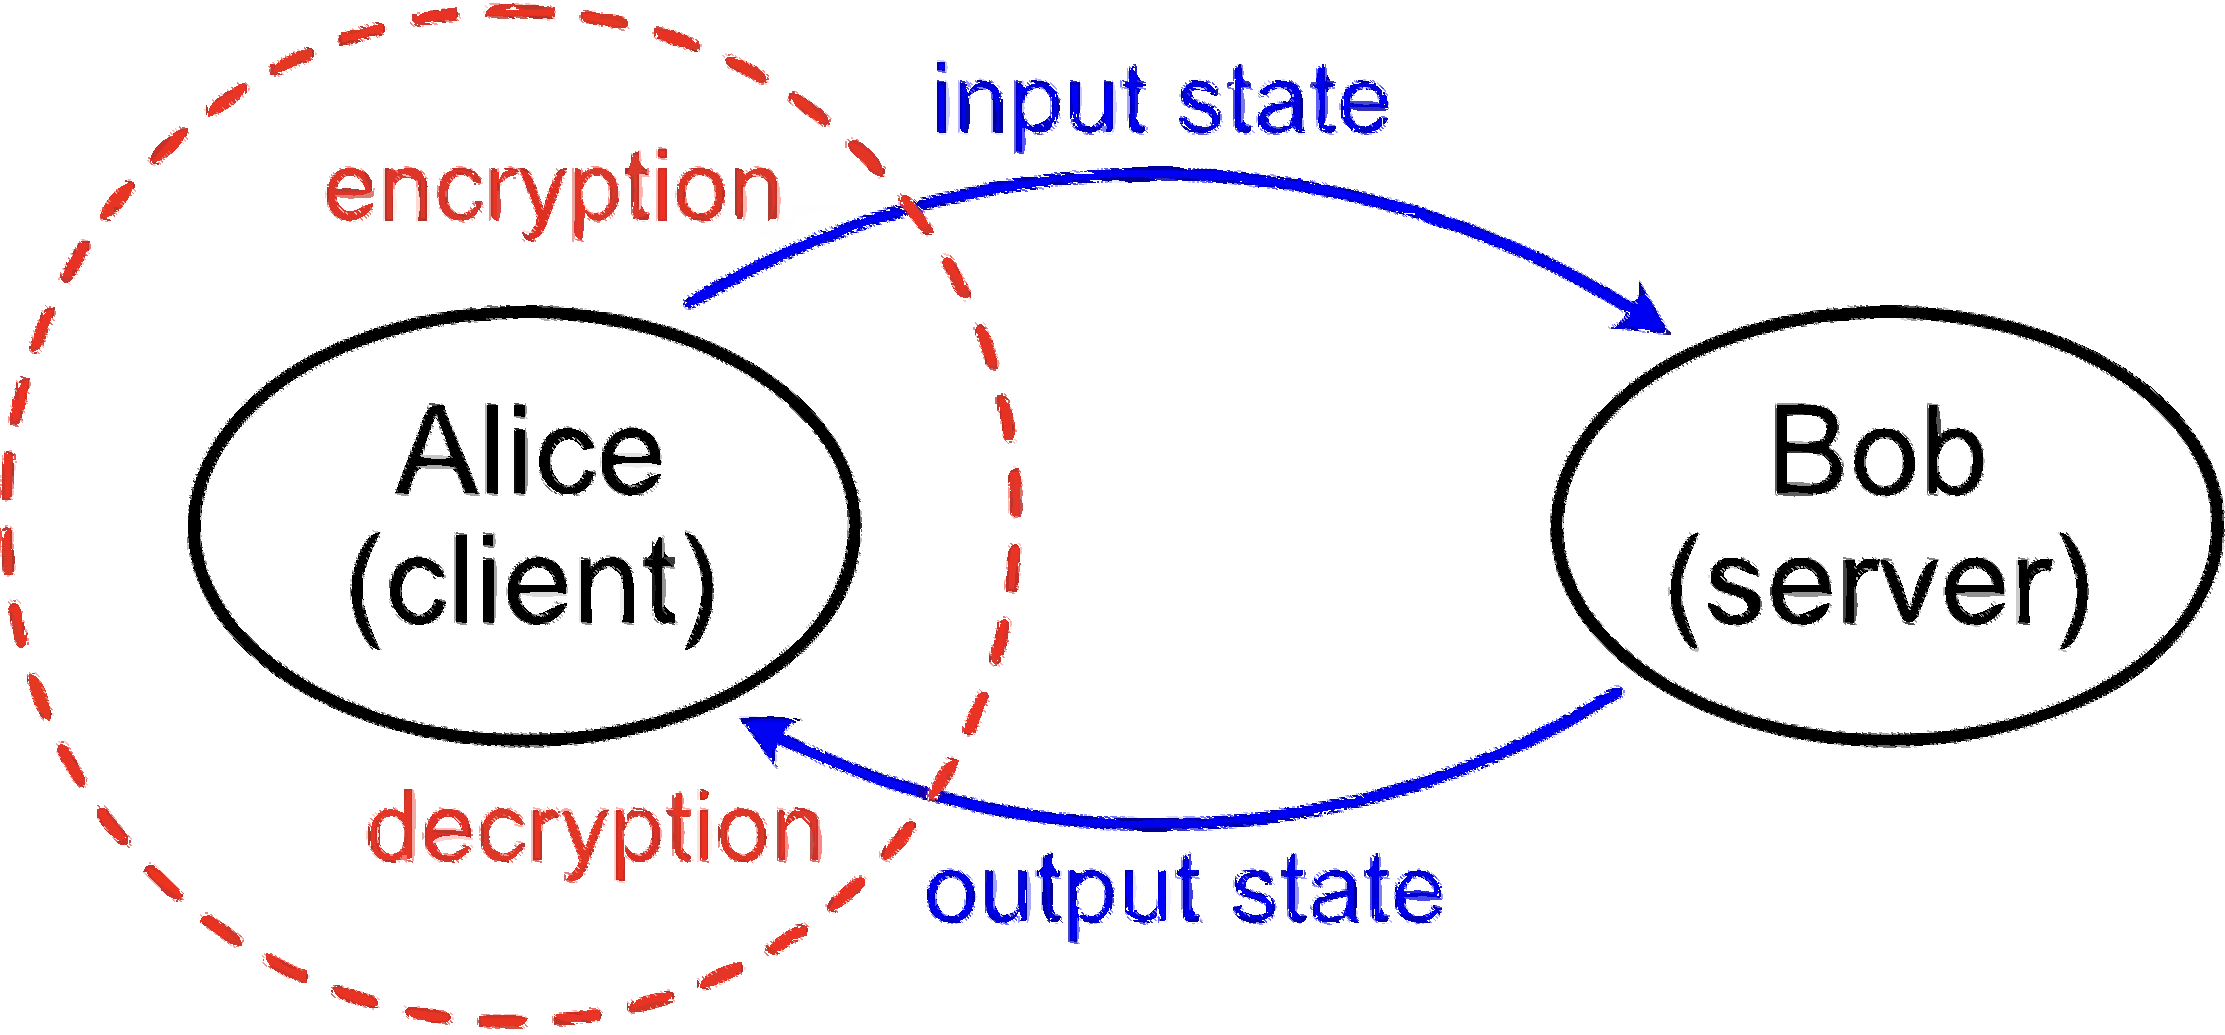
\includegraphics[width=\columnwidth]{figures/QHE}
	\caption{Quantum homomorphic encryption. Alice wishes to securely outsource a computation to Bob. Alice sends encrypted data and requires that the computation be implemented on the data in encrypted form, without first requiring decryption. The encrypted output to the computation is returned to Alice who is able to decrypt it.} \label{fig:QHE_model}
\end{figure}

Classically, homomorphic encryption is possible but highly impractical for most purposes \cite{bib:Gentry}. However, numerous approaches have been described for \emph{quantum homomorphic encryption} (QHE) \cite{bib:BJe15, bib:DSS16, bib:ouyang2020homomorphic, bib:TKOCF-qhe}. This isn't possible using only classical communication between the client and server. Instead we impose minimalistic resources for the client, comprising only state preparation, measurement and teleportation, whereas the server has arbitrary quantum resources (see Fig.~\ref{fig:outsourcing}).

\begin{figure}[!htb]
	\centering
	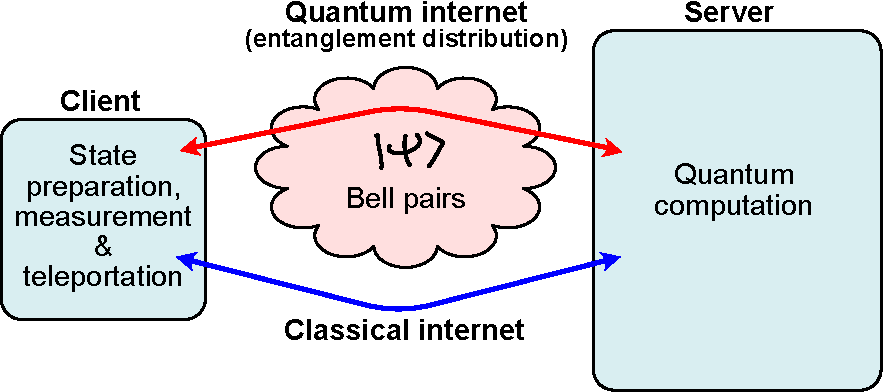
\includegraphics[width=\columnwidth]{figures/QC_outsourcing_model.pdf}
	\caption{Model for outsourced quantum computation using quantum homomorphic encryption. The client is assumed to have minimal quantum resources: state preparation, measurement and teleportation. The server has arbitrary quantum resources for large-scale quantum computation.} \label{fig:outsourcing}
\end{figure}

Perhaps the easiest to explain is QHE of Clifford circuits, which have the property that they commute with the Pauli group, satisfying,
\begin{align}
	\hat{U}_\mathrm{C} \cdot \bigotimes_{i=1}^n \hat{\sigma}_{f(i)} = \bigotimes_{i=1}^n \hat{\sigma}_{g(i)} \cdot \hat{U}_\mathrm{C},
\end{align}
where $\hat{U}_\mathrm{C}$ is a Clifford circuit, $\hat{\sigma}_i$ are the Pauli operators, and the functions $f(i)$ and $g(i)$ characterise the commutation relation between the Pauli operators and the Clifford circuit.

Suppose Alice wants to outsource her state $\hat\rho$ to the server who implements $\hat{U}_\mathrm{C}$. She encrypts it by applying one of the four Pauli operators to it, according to her key \mbox{$f(i)\in\{0,1,2,3\}$}, which is uniform and random,
\begin{align}
	\hat\rho_{\rm Alice}^{\rm enc} = \hat\sigma_{f(i)} \hat\rho_{\rm Alice} \hat\sigma_{f(i)}.
\end{align}

The server or any eavesdropper in the absence of knowing the key would observe the state,
\begin{align}
	\hat\rho_{\rm Bob}^{\rm enc} = \frac{1}{4}\sum_{k=1}^4 \hat\sigma_k \hat\rho \hat\sigma_k = \frac{\hat{I}}{4},
\end{align}
which is the completely mixed state. Since this is independent of $\hat\rho$, no information about Alice's input or output state can be known. Thus, this scheme offers information-theoretic security. Equivalently, the mutual information between Alice and Bob is identically zero,
\begin{align}
	I(A:B) = 0.	
\end{align}

Upon receiving the output, Alice can decrypt her qubits using the commuted key $g(i)$, which can be efficiently classically calculated from $f(i)$ for Clifford circuits. The model is shown in Fig.~\ref{fig:QHE_Clifford}.

\begin{figure}[!htb]
	\centering
	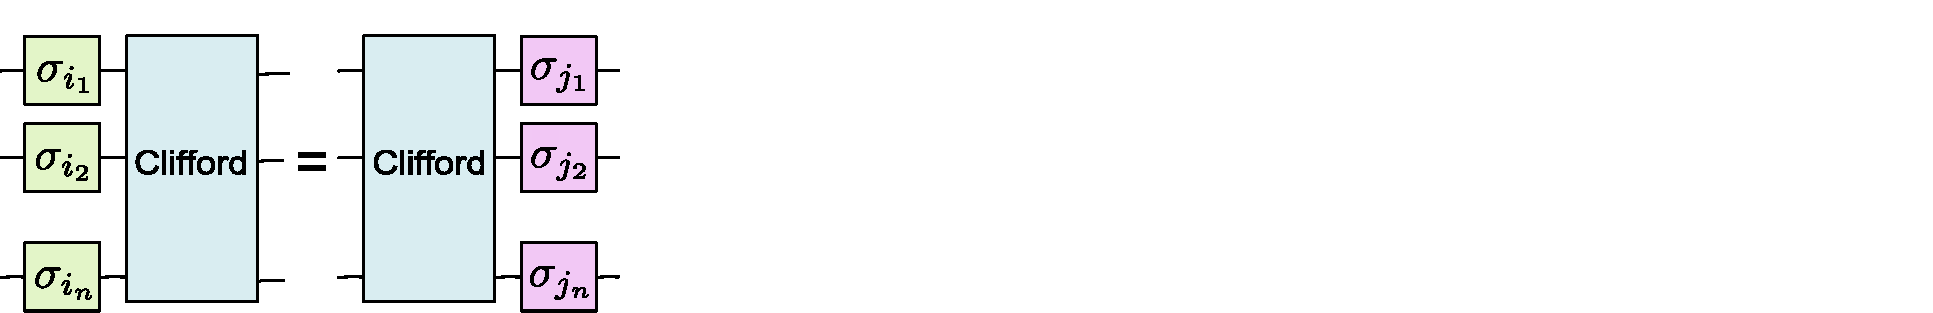
\includegraphics[width=\columnwidth]{figures/Clifford_QHE}
	\caption{Homomorphic encryption of Clifford circuits using Pauli-key encoding. This construction offers perfect information-theoretic security to Alice since the server, in the absence of knowing the key, observes a completely randomised state.} \label{fig:QHE_Clifford}
\end{figure}

The quantum computer scientists are protesting at this point that Clifford circuits are not universal for quantum computing and can be efficiently classically simulated. This is true if the input states are Clifford states, however by injecting so-called \emph{magic states} (single-qubit states of a particular form that facilitate the implementation of $T$-gates via gate teleportation), Clifford circuits can indeed be made universal for quantum computation.

A similar idea can be applied to linear optics circuits, with whom optical displacement operators, $\hat{D}(\alpha)$, commute to yield a different set of displacement operators,
\begin{align}
	\hat{U}_\mathrm{LO} \cdot \bigotimes_{i=1}^n \hat{D}_i(\alpha_i) = \bigotimes_{i=1}^n \hat{D}_i(\beta_i) \cdot \hat{U}_\mathrm{LO},
\end{align}
where $\hat{U}_\mathrm{LO}$ is a linear optics circuit comprising beamsplitters and phase-shifters, and $\hat{D}_i(\alpha_i)$ are the displacement operators on mode $i$.

The commutation relation for displacement operators acting on linear optics networks is classically efficient and obtained by simple matrix multiplication,
\begin{align}
	\vec\beta = U_\mathrm{LO}\cdot\vec\alpha.	
\end{align}

Displacement operators are easily experimentally realised using beamsplitters and coherent states produced by laser sources. This paves the way for QHE to be applied to linear optics quantum computations \cite{bib:KLM01} (see Fig.~\ref{fig:QHE_LO}).

\begin{figure}[!htb]
	\centering
	
\includegraphics[width=\columnwidth]{figures/LO_QHE}
	\caption{Homomorphic encryption of linear optics circuits using displacement-key encoding.} \label{fig:QHE_LO}
\end{figure}

\subsubsection{Blind quantum computing} \label{blind-quantum-computing}

Blind quantum computing (BQC) is a stronger form of outsourced quantum computation whereby both the data \emph{and} the algorithm itself are shielded from the server \cite{bib:FitzsimonsBQC} (see Fig.~\ref{fig:blind_model}). This is particularly important for clients wishing to implement proprietary algorithms of significant value that ought to be protected. The model can be conceptualised as per the figure below.

\begin{figure}[!htb]
	\centering
	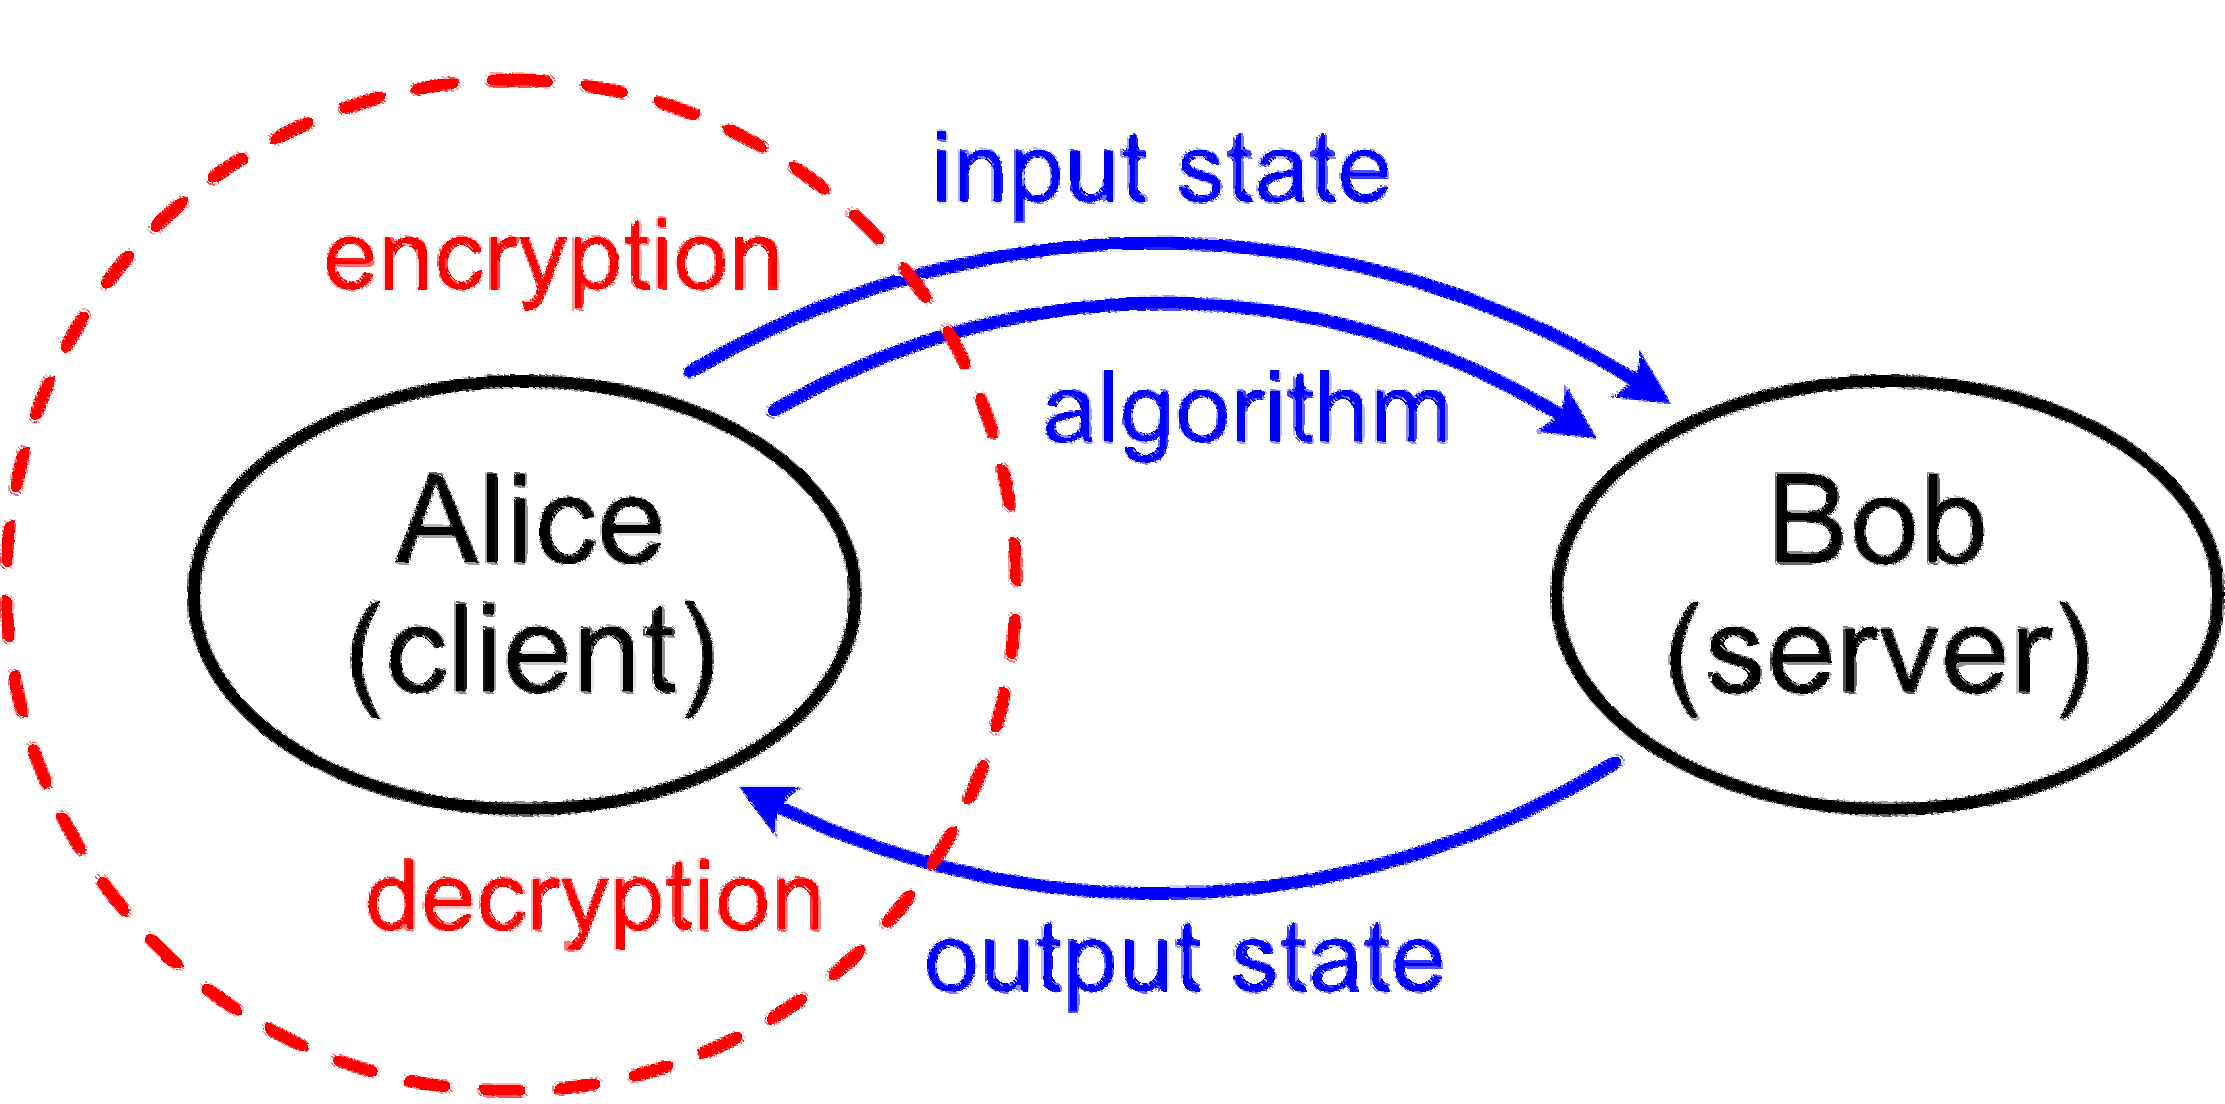
\includegraphics[width=\columnwidth]{figures/BQC}
	\caption{Blind quantum computing is similar to quantum homomorphic encryption, except that in addition to the data being encrypted, the algorithm is also. Bob is required to execute the computation without learning the algorithm or the data.} \label{fig:blind_model}
\end{figure}

While there have been many described variants for implementing blind \emph{quantum} computing, it is known that blind \emph{classical} computation is not theoretically possible.

The easiest model for BQC to describe is via the graph state model for quantum computation. Here a graph state is prepared such that vertices represent qubits and edges represent entangling controlled-phase gates. Graph states are defined only by the graph, with the remainder of the state preparation process being fixed. Formally, a graph state on graph $G=(V,E)$, where $V$ denotes vertices and $E$ denote edges, is defined as,
\begin{align}
	|G\rangle = \prod_{e\in E} \hat{\mathrm{CZ}}_e |+\rangle^{\otimes n},
\end{align}
where there are \mbox{$n=|V|$} qubits, $\hat{\mathrm{CZ}}$ is the two-qubit, maximally entangling, controlled-phase gate, and,
\begin{align}
	|+\rangle = \frac{1}{\sqrt{2}}(|0\rangle + |1\rangle).
\end{align}

Given a graph state of sufficient size, an arbitrary computation can be implemented via single-qubit measurements alone --- the so-called measurement-based model for quantum computation (MBQC) \cite{bib:Raussendorf03}. In the measurement-based model, it is the order and basis in which qubits are measured that defines the algorithm, where the order and basis choice depends upon previous measurement outcomes.

Suppose the server prepares a large graph state. Rather than perform the measurements, it communicates the qubits to the client one at a time, who performs the measurements. Now all the server knows is the graph topology, which is universal and could implement any algorithm up to a given size. This shields the server from knowing anything about the algorithm itself. The client who performs the measurements now has complete control over what algorithm is implemented (via the choice of measurements), and what the output state is (the last measured qubits). The model is shown in Fig.~\ref{fig:blind_MBQC}.

\begin{figure}[!htb]
	\centering
	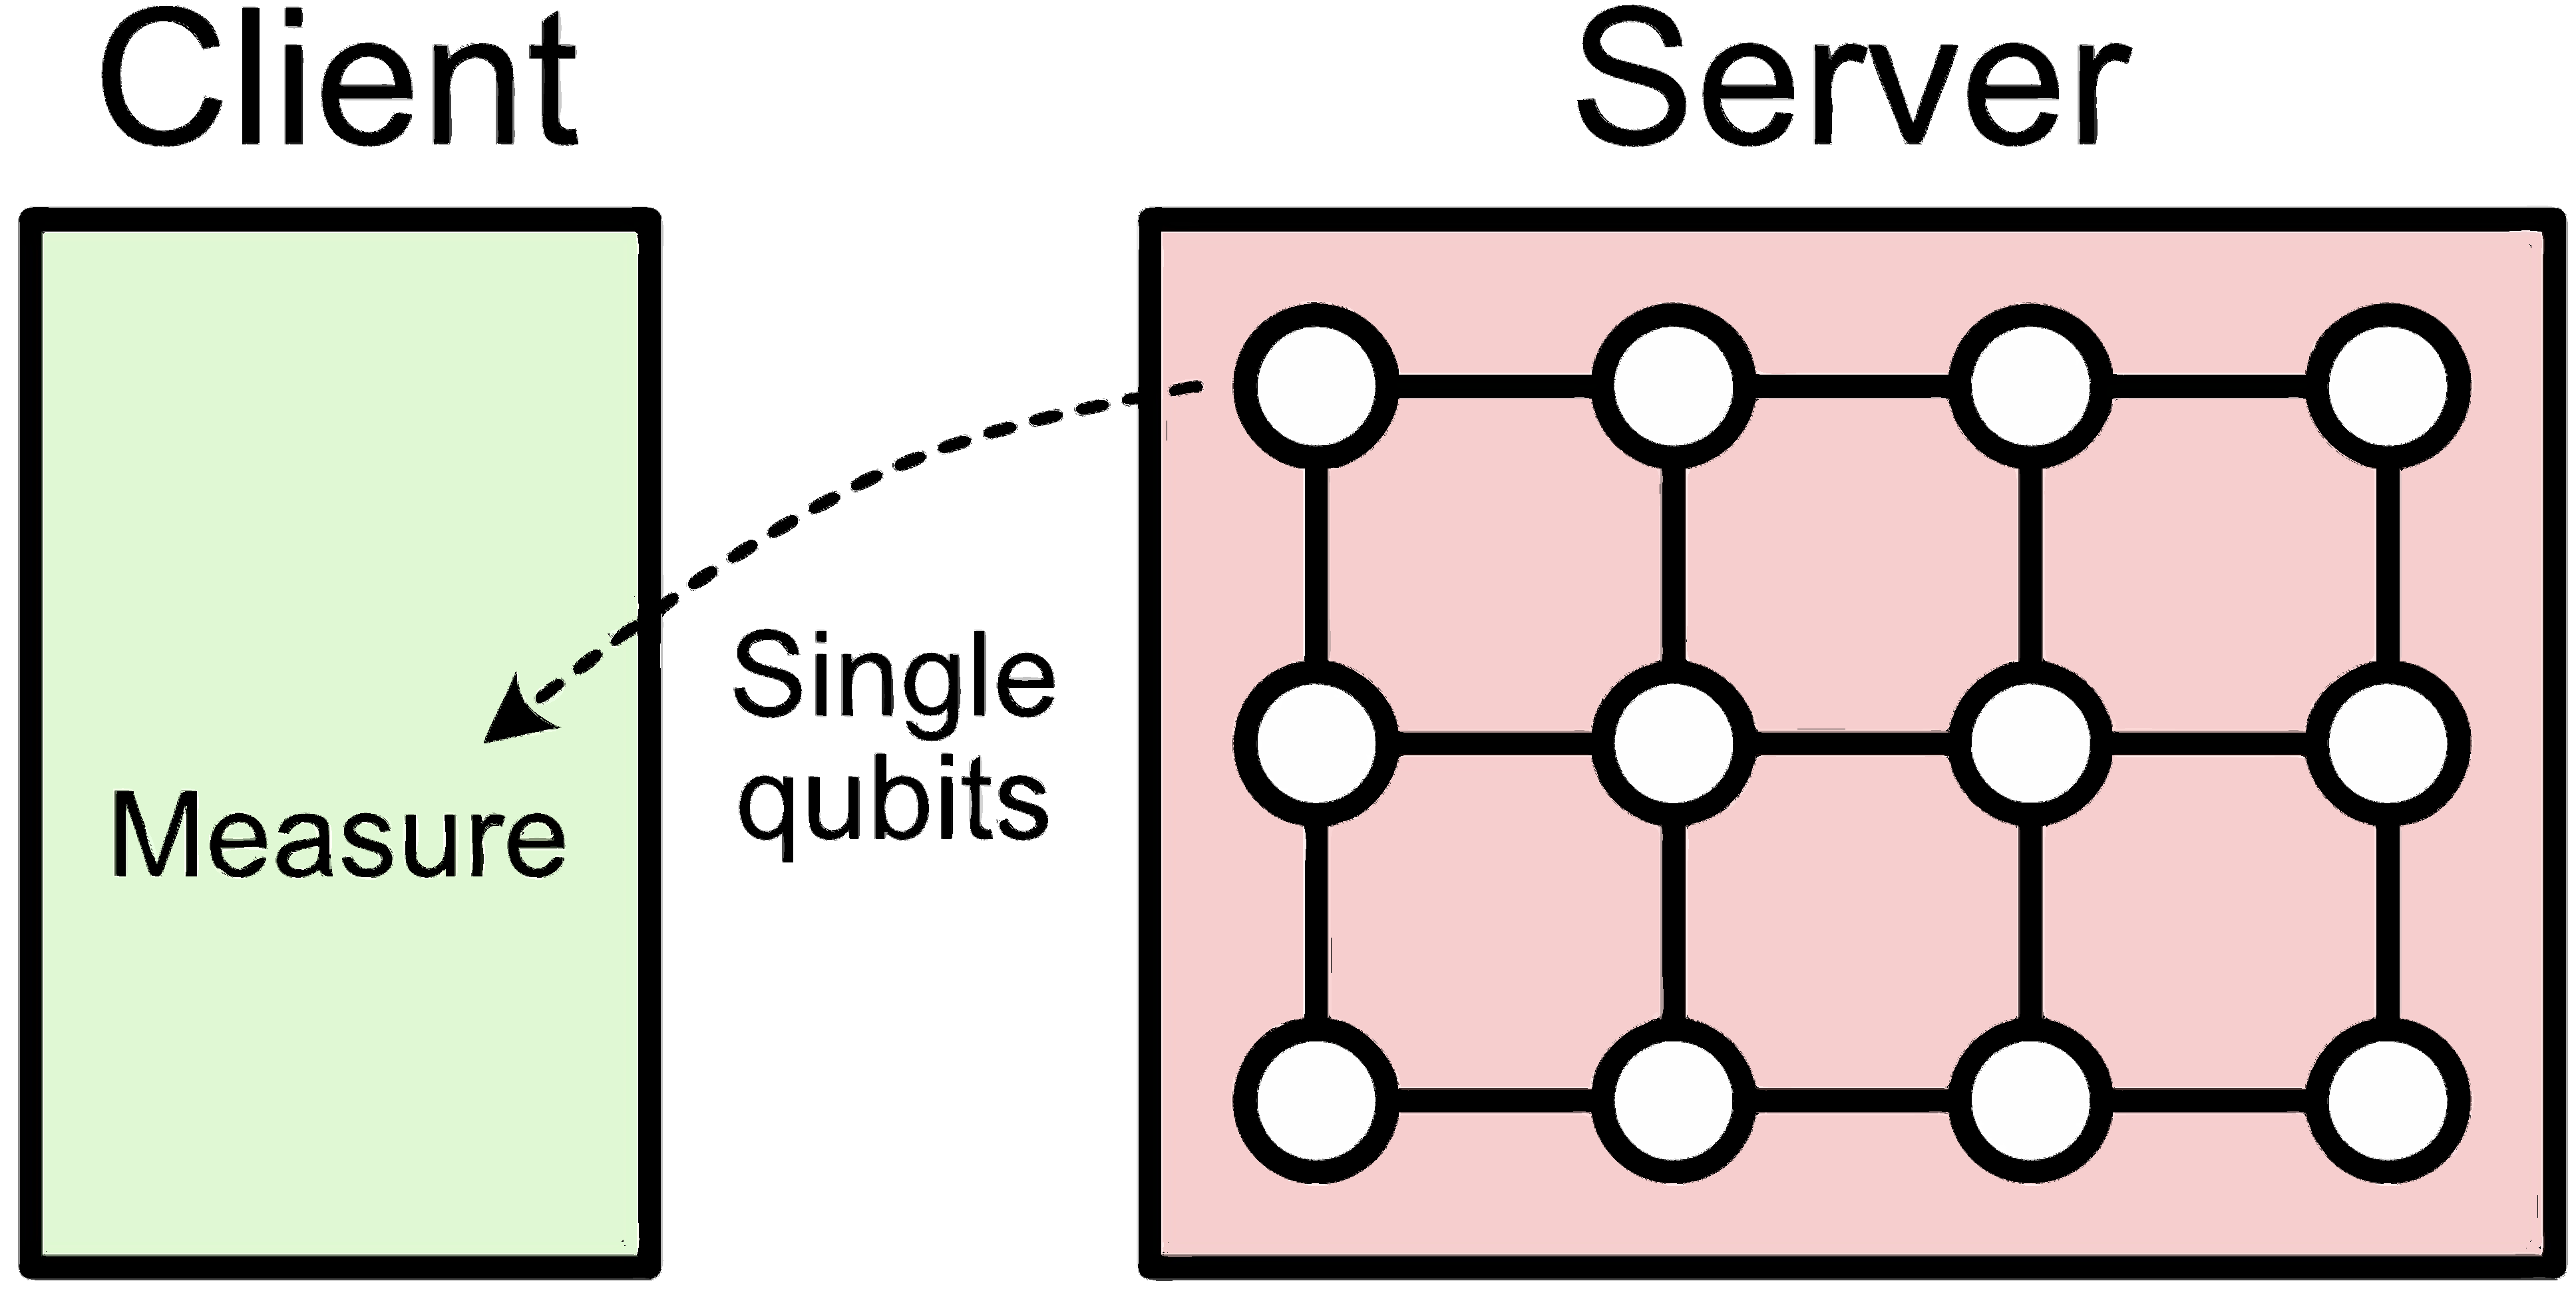
\includegraphics[width=0.75\columnwidth]{figures/BQC_MBQC}
	\caption{One of many models for blind quantum computing using the graph state model for quantum computing. The server prepares the complete graph state and communicates its qubits to the client one at a time for measurement in the appropriate basis.} \label{fig:blind_MBQC}
\end{figure}
\section{Post-quantum cryptography (PQC)} \label{post-quantum-cryptography-pqc}

Despite offering in principle perfect security, there are several major issues with QKD as a form of cryptography that make it undesirable:
\begin{itemize}
	\item Quantum infrastructure is and likely always will be extremely expensive compared to our existing classical infrastructure.
	\item Globally we already have multi-trillion-dollar infrastructure for classical communication that cannot be made compatible with qubits.
	\item That quantum information cannot be broadcast essentially rules it out for mobile or roaming devices.
	\item It requires classical authentication of the public channel.
	\item Keys have one-time use, meaning quantum bandwidth must be extremely high.
	\item It does not facilitate public-key cryptography, only private-key cryptography.
	\item Our existing private-key cryptography is not vulnerable to any known quantum attacks beyond a Grover attack --- easily offset via longer key lengths --- and has the advantage of key reusability.
\end{itemize}

In light of these disadvantages, it would be far more attractive if \emph{classical} encryption techniques could be developed that are both quantum-proof and satisfy our need for public-key encryption and digital signatures. This has now become a major field of research.

If successful, this would imply that becoming cryptographically quantum-proof would become a trivial matter of substituting cryptographic software libraries and all our existing software would be safe. It doesn't take much convincing to see how much more desirable this would be than rolling out trillions of dollars in new infrastructure that only promises improved \emph{private}-key cryptography, which has limited utility in isolation.

\subsection{Hash-based digital signatures} \label{hash-based-digital-signatures}

Hash-based digital signatures are an alternative to RSA/ECC in which the security of signatures is inherited from the pre-image resistance of hash functions --- so long as we employ strong hash functions which are computationally hard to invert, the digital signature will also be secure.

\subsubsection{Lamport one-time signatures} \label{lamport-one-time-signatures}

\begin{figure*}[!htb]
\begin{tabular}{|l|l|l|l|l|}
\hline
\textbf{Bit} & \textbf{Private key} & \textbf{Public key} & \textbf{Message} & \textbf{Signature} \\
\hline
\hline
$1$ & ${\tt priv}_0(1),{\tt priv}_1(1)$ & ${\tt hash}({\tt priv}_0(1)),{\tt hash}({\tt priv}_1(1))$ & $m_1$ & ${\tt priv}_{m_1}(1)$ \\
$2$ & ${\tt priv}_0(2),{\tt priv}_1(2)$ & ${\tt hash}({\tt priv}_0(2)),{\tt hash}({\tt priv}_1(2))$ & $m_2$ & ${\tt priv}_{m_2}(2)$ \\
$3$ & ${\tt priv}_0(3),{\tt priv}_1(3)$ & ${\tt hash}({\tt priv}_0(3)),{\tt hash}({\tt priv}_1(3))$ & $m_3$ & ${\tt priv}_{m_3}(3)$ \\
$4$ & ${\tt priv}_0(4),{\tt priv}_1(4)$ & ${\tt hash}({\tt priv}_0(4)),{\tt hash}({\tt priv}_1(4))$ & $m_4$ & ${\tt priv}_{m_4}(4)$ \\
$5$ & ${\tt priv}_0(5),{\tt priv}_1(5)$ & ${\tt hash}({\tt priv}_0(5)),{\tt hash}({\tt priv}_1(5))$ & $m_5$ & ${\tt priv}_{m_5}(5)$ \\
$\vdots$ & $\vdots$ & $\vdots$ & $\vdots$ & $\vdots$ \\
$n$ & ${\tt priv}_0(n),{\tt priv}_1(n)$ & ${\tt hash}({\tt priv}_0(n)),{\tt hash}({\tt priv}_1(n))$ & $m_n$ & ${\tt priv}_{m_n}$($n$) \\
\hline
\end{tabular}
\caption{Signature scheme for the Lamport hash-based digital signature.} \label{fig:Lamport_sig}
\end{figure*}

The first hash-based digital signature scheme was the Lamport signature \cite{bib:lamport1979constructing}. While the Lamport signature is very strong it has the disadvantage that it is a \emph{one-time signature} --- it can only be used once. This makes it a not-so-useful signature scheme on its own. However, as we will see later, it can be used as a cryptographic primitive for the Merkle Signature Scheme which does allow reusable public keys.

Suppose we want to sign a 256-bit message digest (i.e a 256-bit hash of the full message we are signing). The private and public keys are established as follows:

\paragraph{Private key}

We choose 256 pairs of 256-bit random numbers. For the $i$th pair we denote these two numbers as ${\tt priv}_m(i)$ where $m=\{0,1\}$ index the two numbers in the pair. This has a total memory footprint of 128Kb.

\paragraph{Public key}

The associated public key is the correspondingly indexed set of 256-bit hashes of the private key numbers, such that,
\begin{align}
	{\tt pub}_m(i) = {\tt hash}({\tt priv}_m(i)).
\end{align}
This also has a total memory footprint of 128Kb. Thus the key pair is 256Kb in length.

Alice makes all the numbers comprising ${\tt pub}_m(i)$ public. Note that because of the pre-image resistance of the hash function, no one can determine any of the numbers comprising the private key from their respective publicly available hashes. Hence in this example, the \emph{trapdoor function} is a cryptographic hash function, which to the best of our understanding cannot be strongly compromised by quantum computers (see Grover's algorithm in Sec.~\ref{grovers-algorithm}).

\paragraph{Signing}

Our table of private and pubic keys corresponding to each bit in the message is shown in the table in Fig.~\ref{fig:Lamport_sig}. The signature of the message is made by making public the private keys for the corresponding message bits. That is, if the $n\mathrm{th}$ message bit is 0 we add ${\tt priv_0}(n)$ to the signature, and if it was 1 we add ${\tt priv_1}(n)$ to the signature. %The signature scheme is shown in Fig.~\ref{fig:Lamport_sig}.

Supposing the signature was shared \emph{after} the public key was made public, by selectively revealing the associated private key strings, their pre-image resistance implies they must have been known beforehand to whoever made the signature. ???? IS THIS TIMING ARGUMENT RIGHT

The reason the key is one-time is because each time it is used we reveal a part of the private key, thereby opening avenues for the associated bits to be fraudulently signed, and after a moderate number of reuses of the key-pair all private key strings will be known and any message can be fraudulently signed.

\subsubsection{Merkle Signature Scheme} \label{merkle-signature-scheme}

The Lamport signature is extremely secure, so long as the underlying hash function satisfies our cryptographic criteria, which to the best of our understanding contemporary hash functions like SHA-256 do. However, their one-time nature provides them with highly limited utility. What we really need is signatures that can be reused many times, like existing RSA and ECC schemes. To achieve this, using Lamport signatures as the basic building block, reusable signatures can be made by combining them with Merkle tree data structures.

Merkle trees are tree graphs where every node is labelled by the hash of its concatenated child node labels (see Fig.~\ref{fig:Merkle}), 
\begin{align}
	\mathtt{parent}=\mathtt{hash}(\mathtt{child}_1|\dots|\mathtt{child}_n).
\end{align}
This bestows the property that the labels of parent nodes can always be calculated if the labels of their child nodes are known, but not vice-versa owing to the hash function's pre-image resistance property.

\begin{figure}[!htb]
	\centering
	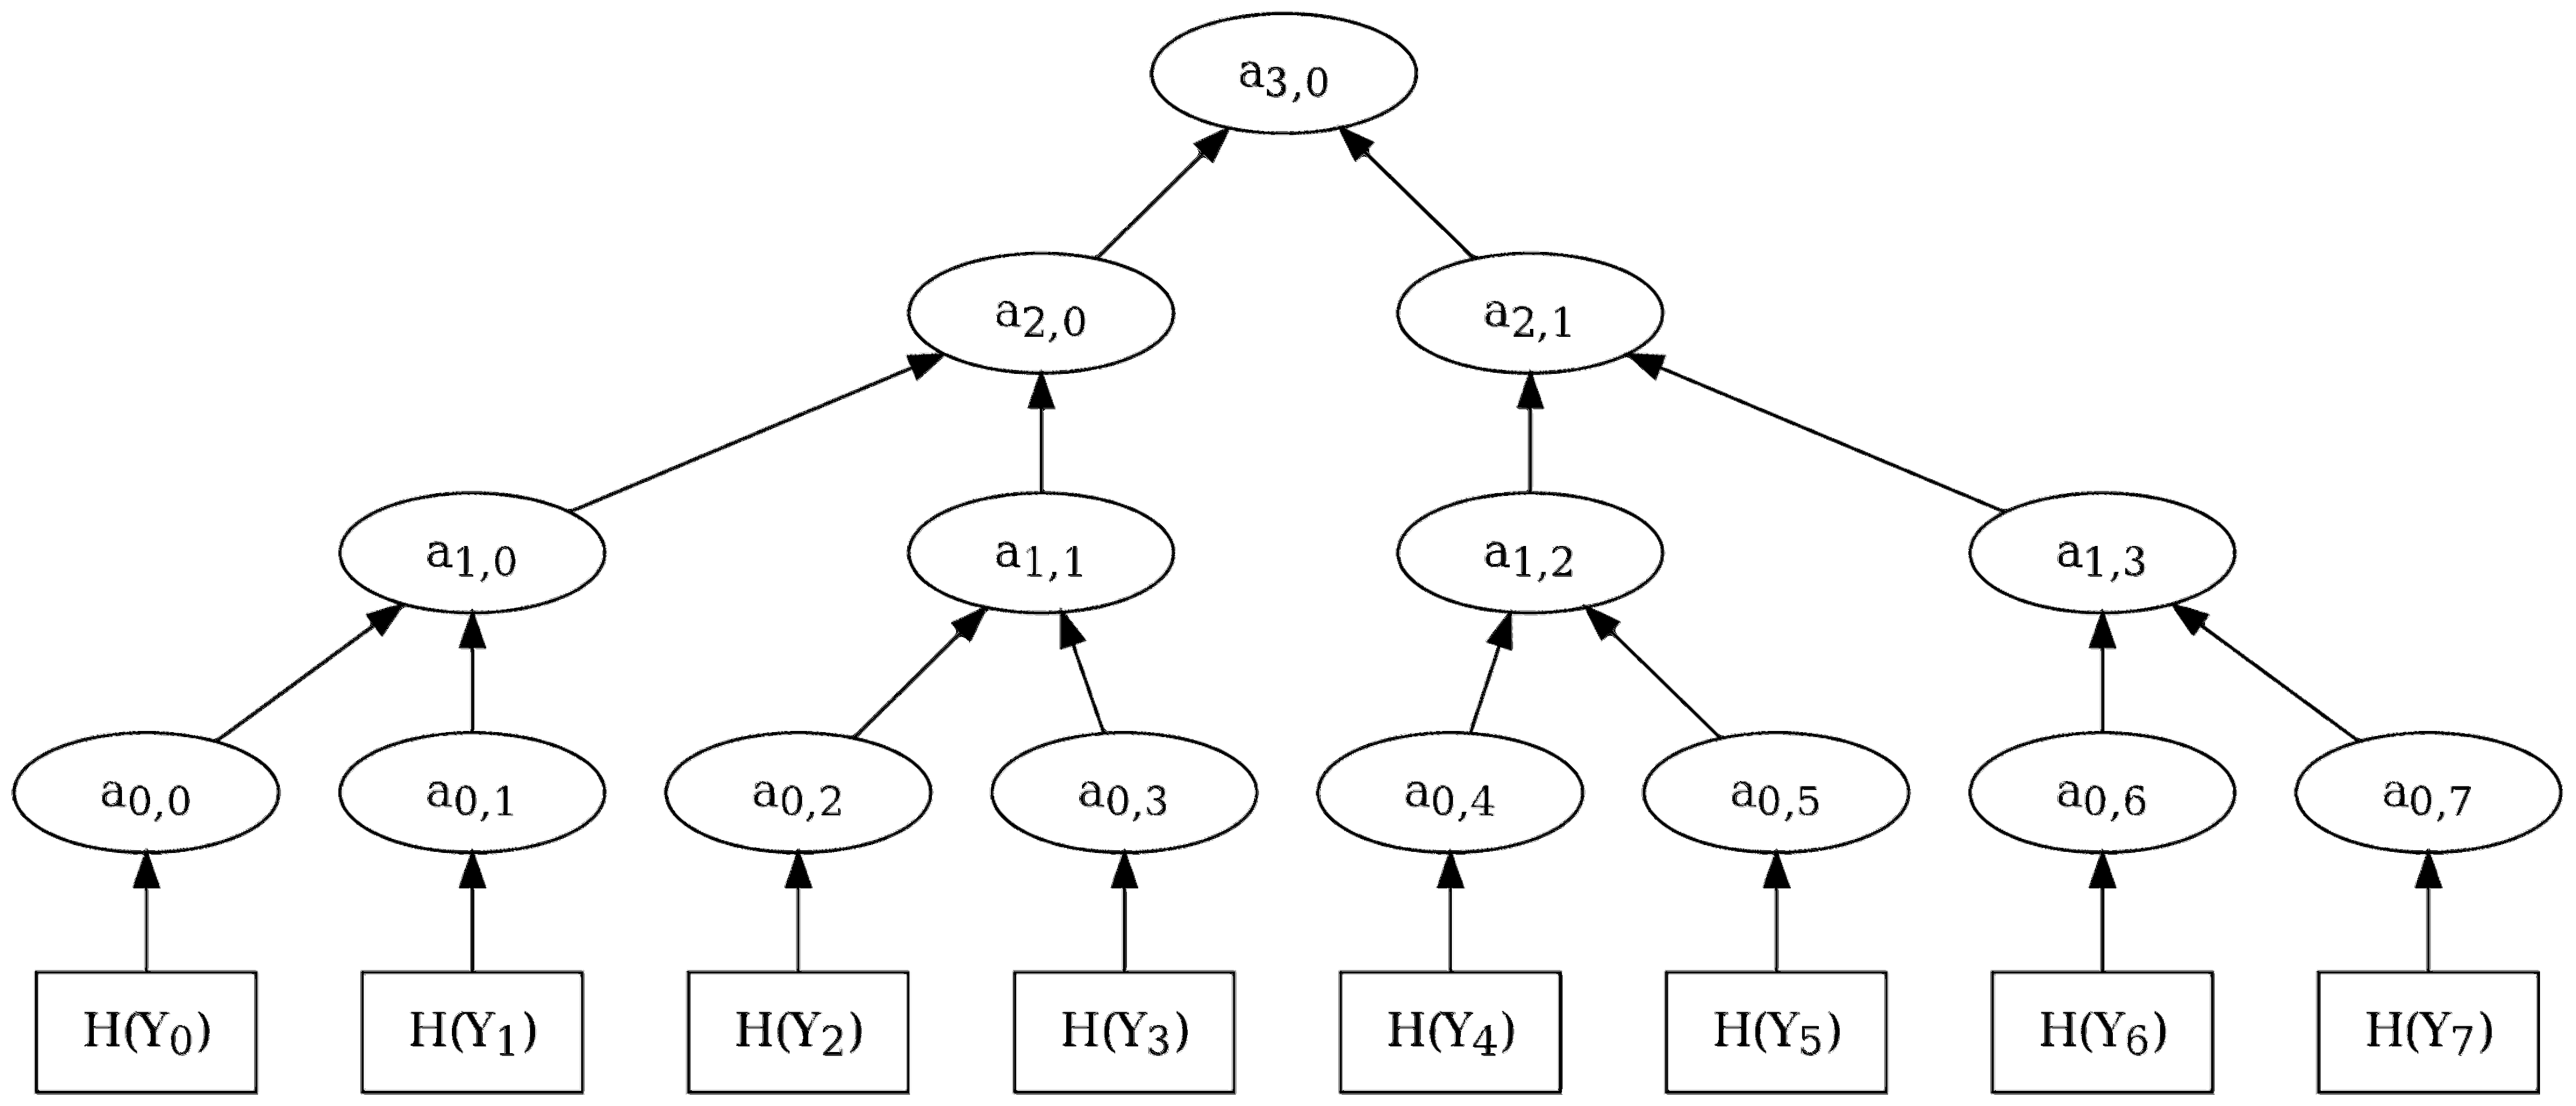
\includegraphics[width=\columnwidth]{figures/Merkle_tree}
	\caption{A Merkle tree data structure. Each node is labeled by the hash of the concatenated labels of its children. The pre-image resistance of the hash function implies that parent nodes can be calculated from their child nodes but not vice-versa. (Image from Wikipedia)} \label{fig:Merkle}
\end{figure}

In the \emph{Merkle signature scheme} we take a very large such Merkle tree, where all the leaf nodes are labelled by the public keys of individual one-time Lamport signatures. The reusable master public key is given by the label of the root node at the top of the tree.

We now want to have a mechanism that allows any of the leaf one-time signatures to demonstrably trace back to the master key. Clearly if all the leaf nodes are revealed we can easily do this. But we won't do that since that would carry an enormous memory footprint. We don't need to either, since the master key can be derived from any chain from a leaf node to the root node, provided the necessary child nodes along that path are selectively revealed. This is referred to as an \emph{authentication path}, as shown in Fig.~\ref{fig:auth_path}. Note that only a single leaf node (i.e one-time signature) need be revealed to form an authentication path to the root node.

\begin{figure}[!htb]
	\centering
	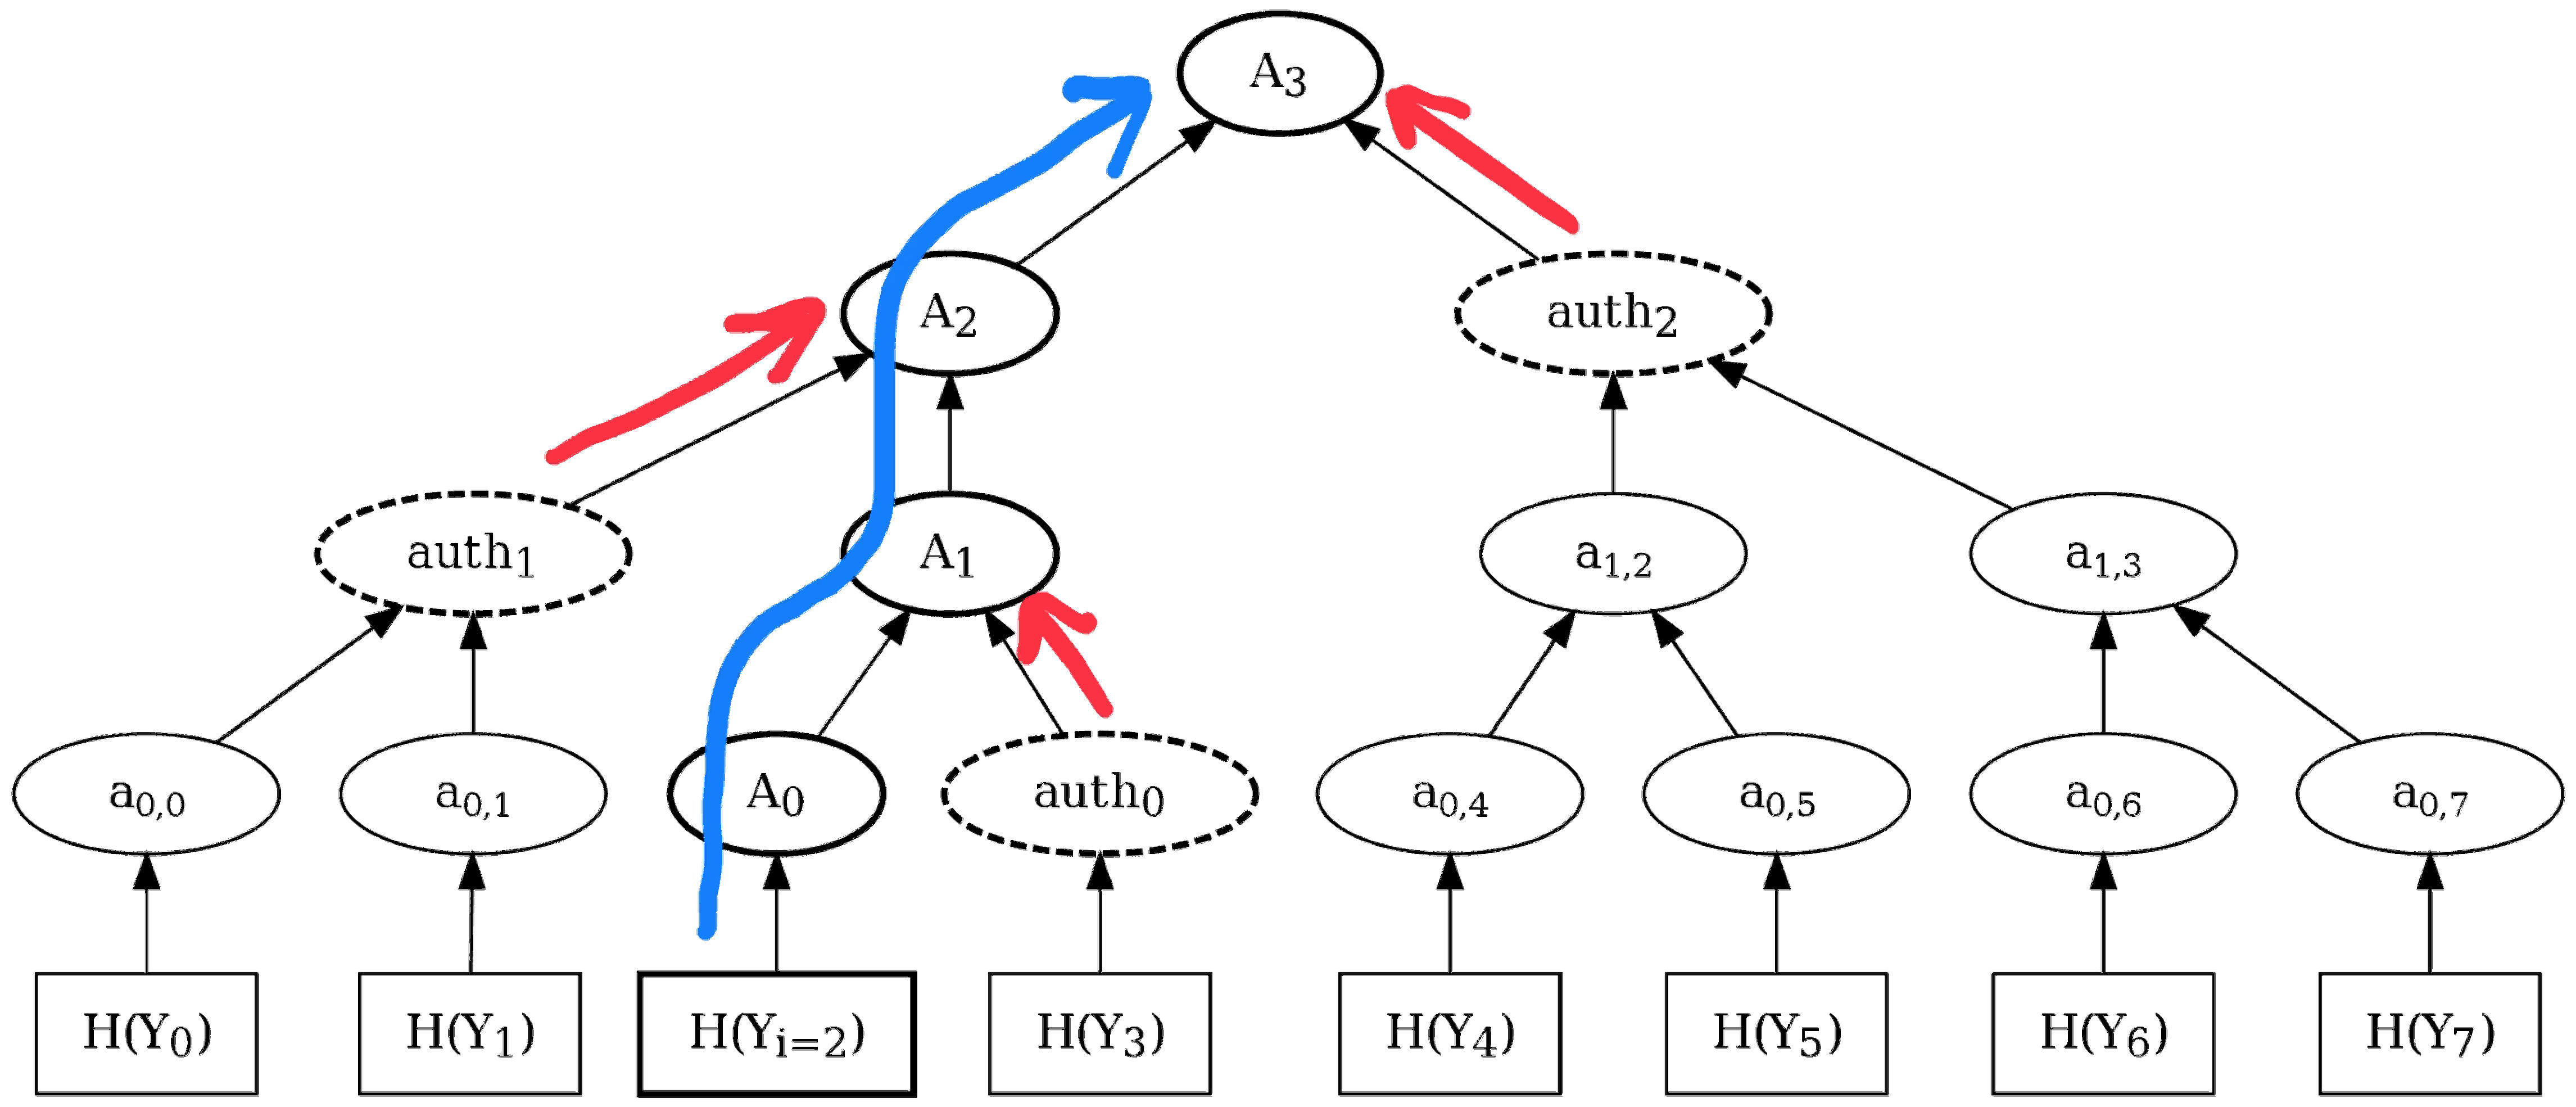
\includegraphics[width=\columnwidth]{figures/Authentication_path}
	\caption{Authentication path for leaf 2. The path to the master key is shown in blue. The additional information that must be revealed to authenticate that path is shown in red. None of the information in the authentication path reveals other leaf nodes based on the pre-image resistance of the hash function. (Image from Wikipedia)} \label{fig:auth_path}
\end{figure}

Since binary trees have depth logarithmic in their number of leaves, this means the size of the authentication chain which must be revealed in order to prove the legitimacy of a single leaf node has only logarithmic overhead in the reusability of the master key, a very efficient overhead. If we consider that $2^{32}\approx 4.3\times 10^9$, this means with a measly factor of 32 overhead in the size of our signatures we are able to have a master public key that can be reused 4.3 billion times. The caveat is that the entire Merkle tree with 4.3 billion key-pairs must be prepared in advance and held by the signatory.

Since the invention of the Merkle signature scheme, various other hash-based schemes have been developed also, such as the Extended Merkle Signature Scheme (XMSS) \cite{bib:XMSS}.

\subsection{Lattice-based cryptography} \label{lattice-based-cryptography}

In addition to the approach of hash-based digital signatures in which only symmetric-key cryptography is used, cryptographers have been looking into the possibility of constructing public-key cryptography based on the hardness of solving certain problems in high-dimensional lattices.  A lattice is a discrete subgroup in a euclidean space $\mathbb R^n$, or the set of all linear combinations of a basis for $\mathbb R^n$ with integer coefficients.  Like a euclidean space, a lattice can have many bases, some of which are ``nicer'' than others in the sense that certain problems are easier to solve in a nice basis.  For example, the problem of finding the shortest (nonzero) vector (SVP) is believed to be hard in a not-so-nice basis.  Furthermore, we do not know any quantum algorithms that have nontrivial speedup over the best classical algorithms for solving certain lattice problems, making these problems a good starting point for constructing PQC.

(??? Details on Kyber, Dilithium, and Falcon, the lattice-based PQC newly standardised by NIST. ???)

\subsection{Standardisation} \label{standardisation}

As with all the major cryptographic primitives we rely on today (e.g AES, SHA, RSA, ECC) they tend to only achieve widespread trust and adoption once they become standardised. Once standardisation takes place, software libraries implementing these primitives will emerge to substitute in for our existing ones and developers will have confidence in the ability for their cryptographic techniques to be interoperable with others.

Currently in the United States the National Institute of Standards \& Technology (NIST) is in the process of standardising post-quantum cryptography. This process will likely still take some time --- cryptography is a highly nuanced and complex field and standardisation sets a high bar for testing and verification. However once this process is complete, we can reasonably expect that post-quantum cryptography will become the norm and switching to post-quantum cryptography will be as simple as substituting software libraries.

Further details about NIST's post-quantum standardisation project can be found at \cite{bib:NIST_PQC}.

\subsection{Outlook}

Although the promise of PQC is quantum resistant public-key cryptography, this is something that is \emph{believed} rather than \emph{proven} to be the case, in the same way that RSA/ECC are believed to be robust against classical attacks but not proven to be so.

In the absence of formal mathematical proofs of their security, the real integrity test of PQC will be the test of time. We can have very high confidence that RSA/ECC are robust against classical attacks, simply because if anyone had found such an attack we would almost certainly know about it by virtue of us all having empty wallets. In effect there is an enormous cash prize for any hacker able to compromise RSA/ECC, and the failure of anyone to claim it implies a high level of confidence in their integrity.

Similarly, as PQC becomes standardised and sees widespread adoption our level of confidence in its integrity will be a function of the test of time as adversaries put it to the test using both classical and future quantum techniques. It would be a mistake to simply take for granted at the point of standardisation that PQC algorithms are as robust as advertised.
\section{Hybrid cryptography} \label{hybrid-cryptography}

Since messages can be multiply encrypted using different keys and different protocols it is often wise to do so. This was the exact principle behind:
\begin{itemize}
	\item Multi-path routing in trusted node QKD networks.
	\item Classical ratchets as employed, for example, by the Signal protocol.
	\item Diffie-Hellmann key exchange, in which the master key is established via communication in \emph{both} directions.
\end{itemize}
Indeed, no matter how secure a protocol is considered to be, it is wise to employ redundancy in encryption on the basis that with multiple encryption \emph{all} layers of encryption must fail in order for it to fail at all.

In the context of military conflict it would be extremely unwise to rely exclusively on QKD for top-secret communications, as it would be very easy to disable the means of communication via denial-of-service attack. It would instead be more preferable to use hybrid quantum/classical encryption, such that if the QKD link fails the classical backup channel remains available. This would ensure maximum security when both channels are available, but in the worst case would reduce to the security of the classical channel alone. This creates a system that in the best case is more secure than relying on either protocol alone, but in the worst case as secure as one of them. When large-scale QKD becomes available, it would be foolish to rely on it alone.

Similarly, since post-quantum encryption is very new and less well studied than existing public key encryption techniques, we might be a little nervous at the thought of immediately switching over to it completely. What if someone clever finds a previously unknown vulnerability?

To offset this anxiety we can use hybrid schemes where we simultaneously use both conventional RSA/ECC public key cryptography and say lattice-based cryptography. Similar to the ratcheting and multi-path QKD schemes, we use both public key encryption schemes to simultaneously share two independent private keys, which we XOR together to create our master private key. This bestows the properly that the master key is secure so long as \emph{at least} one of the individual private keys was secure. That is, the security of the overall scheme is at least as strong as the individual encryption schemes and cannot be worse than either. This provides us with an anxiety-free pathway to transition to post-quantum encryption, without the worry that because it's so new and not as well studied it might have presently unknown vulnerabilities.

OpenSSH, a protocol for creating secure tunnels for remote login, recently announced \cite{bib:OpenSSH} a transition to this methodology, where existing ECC encryption is paired with NTRU lattice-based cryptography to create a scheme believed to be robust against future quantum computers. But if it turns out for whatever reason that NTRU is not as secure as currently understood, the protocol remains at least as strong as the existing ECC algorithm. From their release notes:

\begin{quote}
``The NTRU algorithm is believed to resist attacks enabled by future quantum computers and is paired with the X25519 ECDH key exchange (the previous default) as a backstop against any weaknesses in NTRU Prime that may be discovered in the future. The combination ensures that the hybrid exchange offers at least as good security as the status quo.''
\end{quote}

The philosophy here is that a cryptographic algorithm represents a point of failure should it be compromised and a single point of failure compromises the entire system. By using multiple layers of encryption we create a system that requires multiple points of failure to fail.
\section{Cryptocurrencies \& the blockchain} \label{cryptocurrencies-the-blockchain}

One especially noteworthy contemporary application for cryptography is in the construction of blockchains, which form the basis of cryptocurrencies and smart contract platforms. Conventionally, electronic transactions relied on trusted authorities for authorisation. For example, in a regular online bank transaction the bank itself acts as the trusted authority. This requires absolute trust in a centralised agency.

The goal of blockchain technology is to enable transactions in a trustless environment where there is no centralised, trusted authority. This requires \emph{distributed consensus algorithms} to replace trusted authorities. For this to function in a self-regulating manner there must be mechanisms to both incentivise nodes to participate in consensus, but in a way that prevents collusion and ensures honesty.

\subsection{Proof of work (PoW)}

Proof of work is an approach for randomly choosing a subset of nodes in a network to participate in consensus. In the Bitcoin protocol \cite{bib:NakamotoS} this is referred to as \emph{coin mining}. Proof of work has two purposes:
\begin{itemize}
	\item Who it is that successfully mines coins and participates in subsequent consensus should be inherently randomised to prevent conspiratorial behaviour.
	\item The problem should inherently waste time, so-called `friction'. This restricts the number of nodes likely to succeed. Bitcoin chooses to do this by making users solve inverse hashing problems, whereby an input string to a hash function is deemed to be a coin if its hash has a certain number of leading zeros. As discussed previously, inverse hashing is inherently prohibitive owing to the pre-image resistance of hash functions. Rather than requiring inverting a complete hash we instead require finding a hash output with some adjustable number of leading zeroes, which tune the likelihood of finding a satisfying pre-image, a so-called \emph{partial pre-image} problem. This is how monetary policy is effectively enforced in such protocols where this \emph{difficulty parameter} controls monetary expansion. Specifically, for,
		\begin{align} \label{eq:pow_1}
			x=\mathrm{hash}(y),
		\end{align}
		we wish to find a $y$ such that,
		\begin{align} \label{eq:pow_2}
			x_{1\dots d}=\{0,\dots,0\},
		\end{align}
		where $d$ is the difficulty parameter.
\end{itemize}

In the Bitcoin protocol $x$ is derived from a hash of the  transaction history, such that PoW mining is always unique and associated with the verification of a given transaction.

Due to the unstructured nature of the partial pre-image problem, classical techniques for PoW mining simply rely on brute-force, repeatedly hashing random bit-strings until a satisfying one is found. For difficulty parameter $d$, the likelihood of a single randomly chosen $y$ satisfying Eqs.~\eqref{eq:pow_1} \& \eqref{eq:pow_2} is,
\begin{align}
	P=2^{-d},
\end{align}
and the average number of hashing operations required until a satisfying one is found is,
\begin{align}
	N = \frac{1}{P} = 2^d.	
\end{align}
This enforces our requirement that the choice of nodes participating in the consensus be a small, random subset of nodes and therefore unlikely to be able to collude.

Grover's algorithm (Sec.~\ref{grovers-algorithm}) provides some, albeit limited, quantum advantage here. Although quantum computers cannot efficiently perform inverse hashing, Grover's algorithm has the ability to provide a polynomial speedup in this process by treating inverse hashing as a satisfiability problem. Grover's algorithm in the absence of fault-tolerance overheads provides a quadratic speedup here. What does this translate to in terms of mining? If ordinarily a classical computer would require $2^d$ attempts to successfully find a new coin, a quantum computer could do so using, 
\begin{align}
	O(\sqrt{2^d})=O(2^{d/2}),
\end{align}
	attempts. Although this translates to faster mining, this can be offset by adjusting the difficulty parameter $d$, specifically by doubling it.

Note that proof-of-work is not the only consensus algorithm utilised in blockchains. Indeed, a major criticism of proof-of-work is that the associated friction necessarily wastes compute cycles, resulting in high energy consumption\footnote{The energy consumption associated with the mining necessary to maintain the Bitcoin network is estimated to be on the order of that consumed by a small country, while a single Bitcoin transaction is estimated to consume around \href{https://www.cnet.com/personal-finance/crypto/bitcoin-mining-how-much-electricity-it-takes-and-why-people-are-worried/}{1,449kWh of energy} at the time of writing.}. For this reason many contemporary blockchains have switched to alternate consensus mechanisms such as \emph{proof-of-stake}, whereby participants wager currency to participate in consensus. However proof-of-stake, despite being far more time and energy efficient\footnote{Ethereum's transition to proof-of-stake is touted as being around 99\% more energy efficient than its previous proof-of-work approach.}, is less secure than proof-of-work as it does not ensure randomisation of consensus participants to the extent that proof-of-work does, thereby making it more vulnerable to collusion\footnote{Consensus via a majority vote can be falsified if the majority of participants collude, the so-called `51\% attack'.}.

(??? results from Brennen/Tomamichel on time required to break
blockchains)

\subsection{Distributed consensus}

The proof of work concept is utilised in distributed consensus to randomise which nodes participate. When combined with a reward system, nodes are incentivised to join this lottery. For this reason the proof-of-work stage is also known as \emph{coin mining}, reflecting the associated reward.

Once consensus participants have been determined, they are all required to sign-off on a new transaction for the associated \emph{coin} to be legitimised. Whether the transaction is committed to the blockchain is based on a majority vote by consensus participants. Voters who vote against the majority are considered dishonest and do not obtain the associated reward.

A distributed consensus protocol relying on proof of work is shown in Fig.~\ref{fig:distributed_consensus}.

The sign off stage is implemented using digital signatures, where some standards are vulnerable to quantum attack. The ability to falsify signatures on a blockchain would directly facilitate fraudulent transactions, a major threat to the integrity of the ledger.

It is to be expected that in coming years blockchains will increasingly adopt post-quantum digital signatures. Furthermore, it can be expected that major exisiting blockchains relying on vulnerable digital signatures will undergo \emph{forks} to enable a technology transition to post-quantum cryptography.

`The merge' implemented on the Ethereum blockchain in 2022 in effect substituted major technological implementation details to transition from a proof-of-work (PoW) to a proof-of-stake (PoS) consensus protocol, thereby significantly reducing energy consumption improving efficiency of the Ethereum blockchain. This highly anticipated event was also a highly successful one, with the technological transition seamlessly taking place in the background. Similarly, transitions towards PQC will inevitably become a more common occurrence as the quantum threat begins to materialise.

\begin{figure}[!htb]
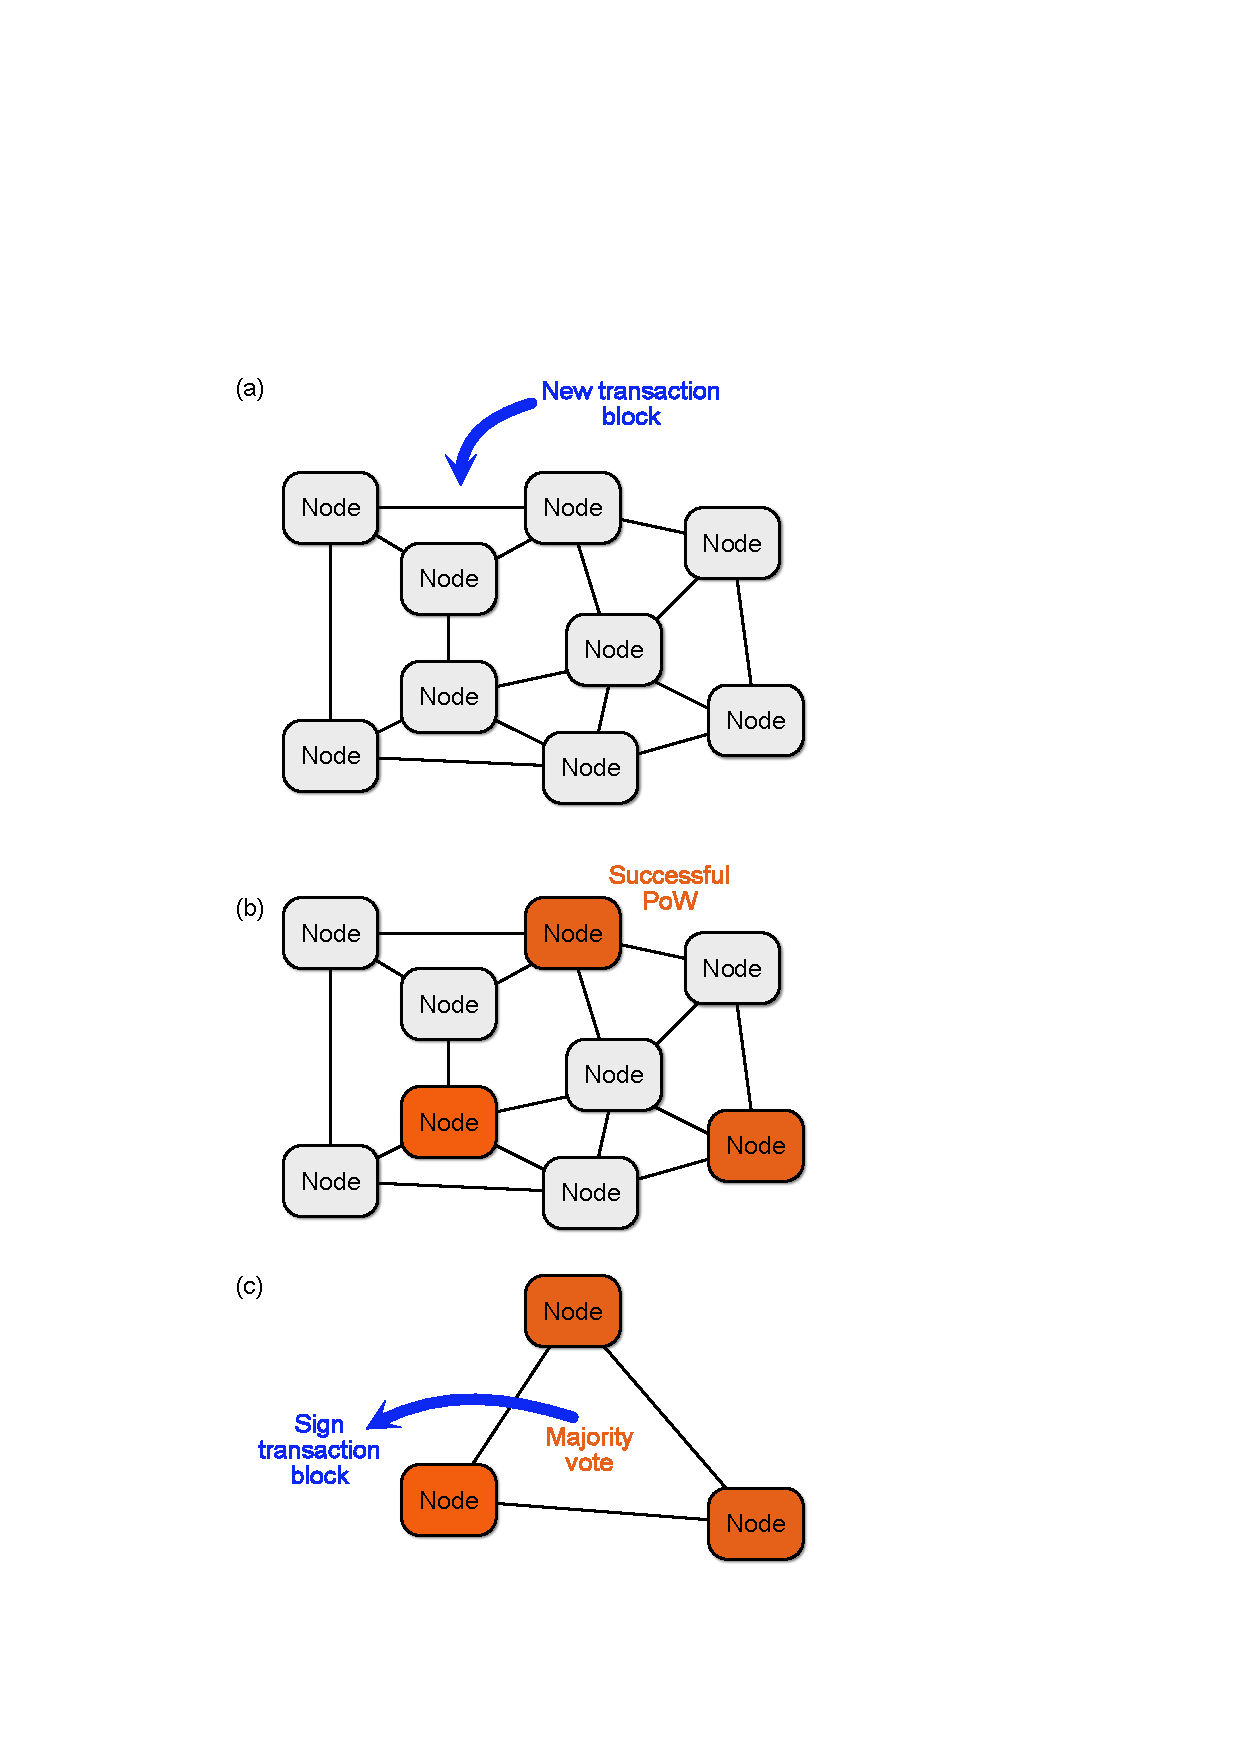
\includegraphics[width=0.8\columnwidth]{figures/distributed_consensus}
\caption{A distributed consensus protocol relying on proof of work to authenticate a blockchain transaction. (a) A network of participating nodes all independently attempt to solve the  proof-of-work problem -- such as the partial pre-image of a hash function -- associated with a new transaction. (b) Due to the unstructured nature of the proof-of-work problem, which nodes successfully solve the problem is inherently randomised, minimising the risk of collusion. (c) The subset of nodes successfully solving the problem sign off on a transaction using digital signatures. The transaction is committed to the blockchain in accordance with a majority vote by consensus participants. Dishonest participants --- ones who vote against the majority --- do not receive their mining reward, thereby incentivising honesty.} \label{fig:distributed_consensus}
\end{figure}

\subsection{Smart contracts}

Many contemporary blockchains accommodate for \emph{smart contracts}, transactions associated with executable code that specify if and under what circumstances the transaction should be executed. This does not rely on any underlying changes to the cryptographic primitives being employed. Rather, it is a higher level abstract layer that sits on top of a protocol relying on existing consensus techniques. Consequently, smart contract platforms are subject to the same vulnerabilities as their underlying blockchain protocol.

\subsection{Distributed autonomous organisations (DAOs)}

One futuristic but currently under-utilised application of smart contract enabled blockchains is the creation of \emph{distributed autonomous organisations} (DAOs). Here we take an entire organisational structure, replacing its administrative components with a framework of smart contracts that algorithmically define and enforce the operational aspects of the organisation. For example, there could be smart contracts associated with payment upon achieving KPIs, or ones enabling members to engage in collective organisational decision making that effectively enforce organisational hierarchy.

DAOs are effectively a further layer of abstraction built on top of a smart contract enabled blockchain. Consequently, their viability and integrity is subject to the same vulnerabilities as the underlying blockchain implementation.
\section{Strategic threats} \label{strategic-threats}

Having presented an overview of the nuances of classical and quantum cryptography, we now delve into the strategic considerations surrounding them and their interplay. A summary of classical and quantum cryptographic primitives and their respective strengths and weaknesses is shown in Fig.~\ref{fig:pros_and_cons}.

\begin{figure*}
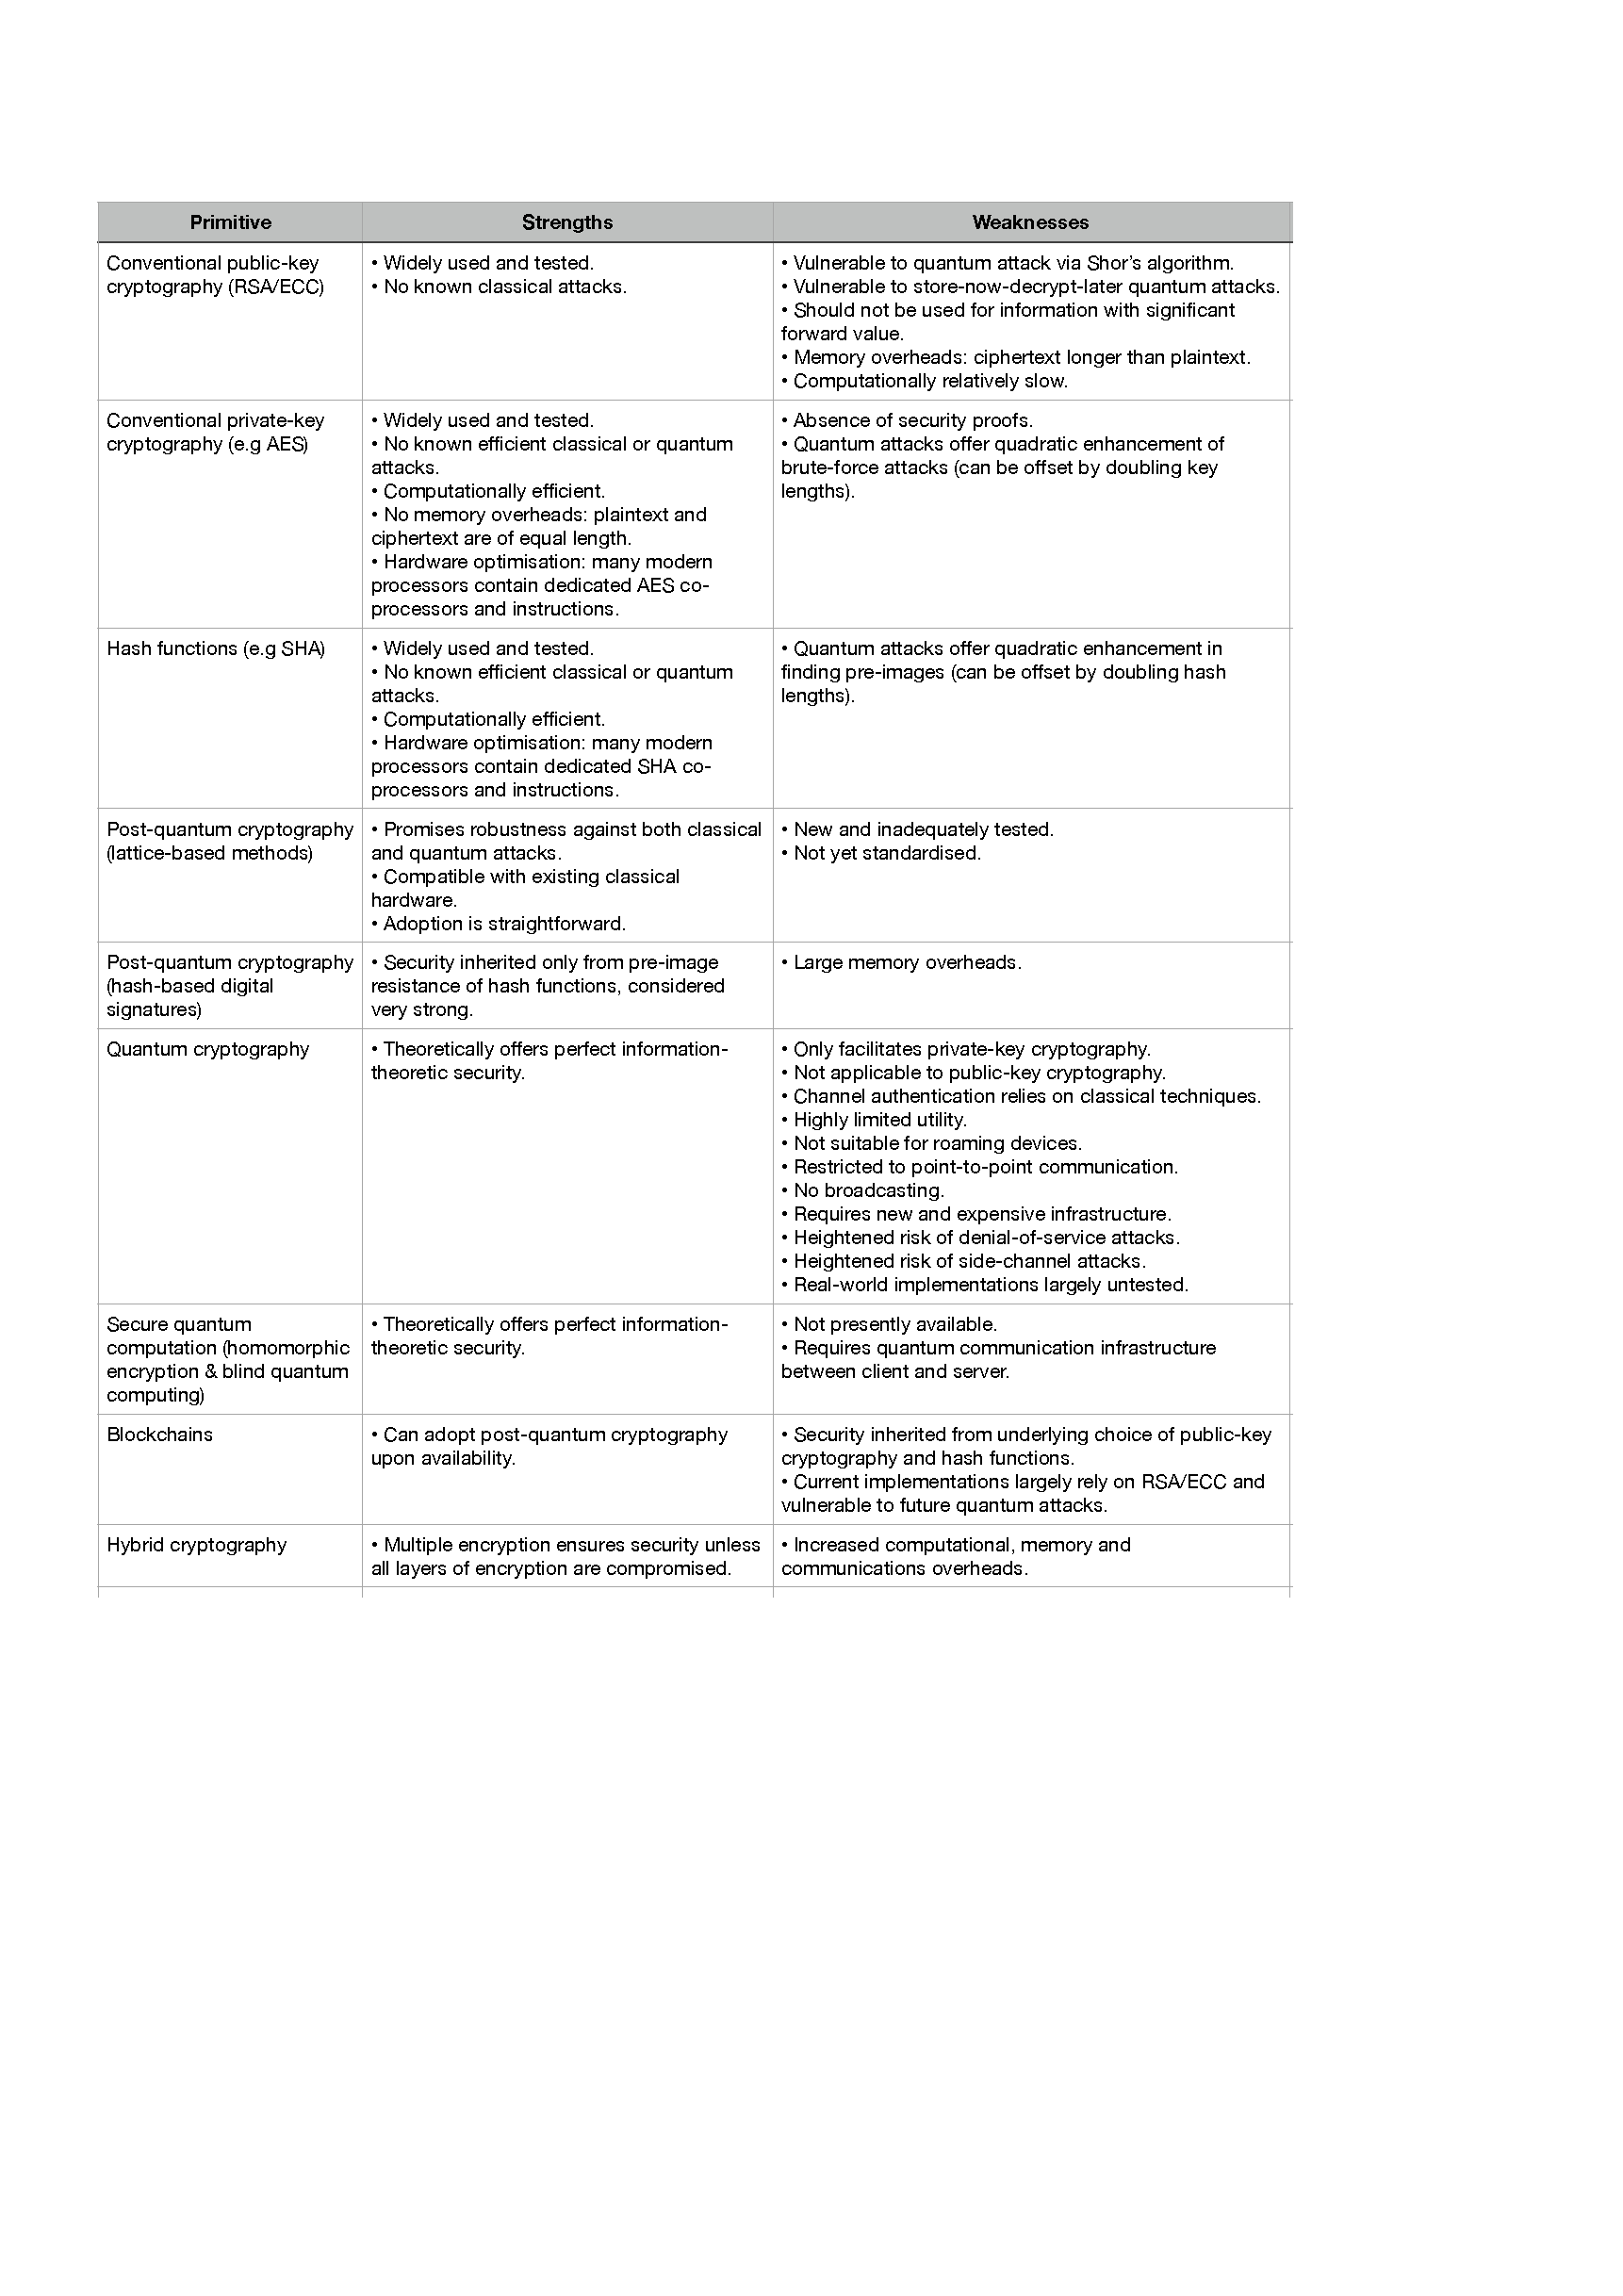
\includegraphics[width=\linewidth]{figures/pros_and_cons}
\caption{Summary of classical and quantum cryptographic primitives and their respective strengths and weaknesses.} \label{fig:pros_and_cons}
\end{figure*}

\subsection{Stored information} \label{stored-information}

While quantum computers of sufficient size to compromise current public key cryptography are likely on the order of a decade or two away, the threats they present are relevant today. It's well known that signals intelligence (SIGINT) agencies around the world, such as the NSA, store encrypted intelligence data that they are presently unable to crack in case some day further down the line they are able to. Since significant amounts of this data will still have strategic or IP relevance in the future, many are no doubt nervous about the prospects of their information being decrypted by adversaries down the line.

It can be taken for granted that nation states are mindful of this when employing encryption protocols today and actively attempt to future-proof their cryptographic protocols against quantum attack vectors or future advancements in cryptanalysis. It is impossible to know what cryptographic advancements have been made by leading SIGINT agencies --- the NSA is purported to be the world's largest employer of mathematicians and needless to say knows far more about cryptography than what is publicly available. Advanced nation states may or may not have developed and employ post-quantum cryptography as part of their cryptographic suites. However what is highly likely is that highly sensitive information is:
\begin{itemize}
	\item Encrypted using keys derived from multiple independent key distribution avenues to minimise the risk of compromised keys being employed.
	\item Multiply encrypted using different encryption algorithms to minimise the risk of unknown vulnerabilities in a given encryption scheme being exploited. PQC would inevitably be a component of such cryptographic suites.
	\item Private keys are derived from multiple independent sources to minimise the likelihood of interception compromising keys.
\end{itemize}

\subsection{Irrelevant information}

While there are troves of data with enormous forward value, to the contrary there are swathes of data of high value today that will be of little or no value tomorrow. Enormous amounts of today's encrypted information will be irrelevant if cracked in the future. For example, when we perform online bank transactions using secure links, once transactions are complete eavesdropping on them is of little value and it isn't possible to manipulate the transaction retrospectively. The issue of \emph{key expiry} is the main point here. If keys are used temporarily for a short period for the sake of some transaction (as opposed to an important communication) and then discarded, this may pose little or no threat.

\subsection{Quantum key distribution}

While QKD offers in principle perfect secrecy of shared bit-strings for use in a one-time-pad or other symmetric cipher, it is far more vulnerable to denial-of-service (Sec.~\ref{denial-of-service-dos-attacks}) and side-channel attacks (Sec.~\ref{side-channel-attacks-qkd}) than classical technology.

Regardless how advanced and mainstream quantum engineering becomes, quantum communications infrastructure will likely always be far more expensive than classical infrastructure. Combined with its more limited use cases this implies quantum networks will be far more sparse than classical ones making them more vulnerable to denial of service attacks.

In the context of military conflict, QKD's vulnerability to denial-of-service is a significant issue, as entities relying on this technology are likely to also be ones of high strategic importance.

QKD will inevitably always be more expensive than classical cryptography, and its use-cases far more limited. Most importantly, QKD only enables private-key cryptography, making it useless for most contemporary applications requiring public-key cryptography. If it is to be used at all, it should be as part of an encryption policy that hybridises it with best-practise classical cryptography, such that the QKD does not act as a single point of failure.

Additionally, quantum information cannot be broadcast in the same way classical information can, rendering it unsuitable for roaming devices on shared networks such as cellular networks.

QKD should be regarded as a technology to compliment rather than replace classical cryptography.

Additionally, it should be noted that secure communications channels additionally require authentication, which reverts back to classical techniques.

Some major Western signals intelligence agencies have released position statements on quantum cryptography. GCHQ, the signals intelligence agency of the United Kingdom \href{https://www.ncsc.gov.uk/whitepaper/quantum-security-technologies}{takes the position},
\begin{quote}
``the NCSC does not endorse the use of QKD for any government or military applications, and cautions against sole reliance on QKD for business-critical networks, especially in Critical National Infrastructure sectors.''
\end{quote}
while the NSA of the United States \href{https://www.nsa.gov/Cybersecurity/Quantum-Key-Distribution-QKD-and-Quantum-Cryptography-QC/
}{takes the similar stance},
\begin{quote}
``NSA views quantum-resistant (or post-quantum) cryptography as a more cost effective and easily maintained solution than quantum key distribution. For all of these reasons, NSA does not support the usage of Quantum Key Distribution or Quantum Cryptography to protect communications in National Security Systems, and does not anticipate certifying or approving any QKD or QC security products for usage by NSS customers unless these limitations are overcome.''
\end{quote}

\subsection{Encrypted computation}

In Secs.~\ref{homomorphic-encryption} \& \ref{blind-quantum-computing} we discussed homomorphic encryption and blind quantum computing, approaches for outsourcing quantum computations such that neither an eavesdropper nor the server performing the computation is able to learn what is being processed.

This brings with it unique strategic considerations in a globalised environment. Since some applications for quantum computing have high strategic or commercial value, enabling adversarial states to opaquely utilise quantum computing infrastructure may pose a strategic threat, one that could be hard to quantify given the secrecy of what is being computed. It would be possible, for example, for an adversarial state to utilise sovereign infrastructure to crack their stored data with high intelligence or intellectual property value.

In some jurisdictions quantum computing is already covered under defence export legislation. It is to be expected that as the field heats up in the coming decades and quantum computers become scalable and capable, so will the regulatory frameworks limiting its use. We might very well see quantum alliances of friendly states who freely share quantum resources, which fracture into a number of discrete strategic quantum alliances.

\subsection{Blockchains} \label{blockchains}

Blockchain based transactions are different however. Since the entire ledger is in the public domain and decentralised --- as opposed to sitting on a private server in a bank vault --- the public ledger could be manipulated if the signature keys of others could be obtained. This could manifest itself via manipulation of the consensus algorithms which sign off on transactions, or by directly compromising individual wallets, both of which are protected using digital signatures. Most major blockchain implementations today rely on signature schemes vulnerable to quantum attack via Shor's algorithms.

\subsubsection{Forward value}

This has major implications for the forward value of blockchains. Based on standard forward value pricing models, if an asset has no future value its discounted present-day value is also zero, and smart contracts aren't very smart if they have been invalidated by the time of maturity \cite{bib:rohdequantcrypto}. For this reason, many blockchains are now under development based on quantum-resistant digital signatures.

\subsubsection{Forks}

\subsection{Caveats} \label{caveats}

It also important to bear in mind that although quantum computers can `efficiently' break RSA/ECC encryption, this doesn't mean they are able to do so spontaneously or cheaply. In fact, running a large scale instance of Shor's algorithm would still take considerable time. This raises two important caveats:
\begin{itemize}
	\item Due to high infrastructural cost compared to classical computing, quantum compute power will be reserved for the highest value applications. Breaking into my personal crypto wallet isn't likely to be one of them, and indeed on a cost benefit analysis probably wouldn't ever be worth it.
	\item Given that quantum computers still take significant time and resources to perform public key code breaking, if the lifespan of keys is below this threshold there isn't likely to be a problem. For example, if blockchains are repeatedly hard-forked and personal wallets given a finite lifetime before they are required to transfer to a new wallet address, the quantum computers won't be able to keep up with the rate of change in signatures. This will create a tit-for-tat situation, as we repeatedly switch our keypairs around, ensuring their lifespan is below threshold.
\end{itemize}
\section{Conclusion} \label{conclusion}

The interplay between information security and quantum technology is both a fascinating and highly non-trivial one that extends far beyond code-breaking and -making. Despite large-scale quantum computing being a long-term objective, the implications are highly relevant today, albeit with many nuances and caveats. Although the technological trajectory is hard to predict, the long term strategic importance of understanding this interplay is already clear and with or without this technology at hand it is essential to keep these implications in mind in any present-day considerations of information security.
\begin{acknowledgements}
Peter Rohde is funded by an ARC Future Fellowship (project FT160100397). This research was conducted by the Australian Research Council Centre of Excellence for Engineered Quantum Systems (project CE170100009) and funded by the Australian Government.
\end{acknowledgements}


\bibliography{bibliography} \label{references}

\end{document}